\documentclass[twoside]{book}

% Packages required by doxygen
\usepackage{calc}
\usepackage{doxygen}
\usepackage{graphicx}
\usepackage[utf8]{inputenc}
\usepackage{makeidx}
\usepackage{multicol}
\usepackage{multirow}
\usepackage{textcomp}
\usepackage[table]{xcolor}

% Font selection
\usepackage[T1]{fontenc}
\usepackage{mathptmx}
\usepackage[scaled=.90]{helvet}
\usepackage{courier}
\usepackage{amssymb}
\usepackage{sectsty}
\renewcommand{\familydefault}{\sfdefault}
\allsectionsfont{%
  \fontseries{bc}\selectfont%
  \color{darkgray}%
}
\renewcommand{\DoxyLabelFont}{%
  \fontseries{bc}\selectfont%
  \color{darkgray}%
}

% Page & text layout
\usepackage{geometry}
\geometry{%
  a4paper,%
  top=2.5cm,%
  bottom=2.5cm,%
  left=2.5cm,%
  right=2.5cm%
}
\tolerance=750
\hfuzz=15pt
\hbadness=750
\setlength{\emergencystretch}{15pt}
\setlength{\parindent}{0cm}
\setlength{\parskip}{0.2cm}
\makeatletter
\renewcommand{\paragraph}{%
  \@startsection{paragraph}{4}{0ex}{-1.0ex}{1.0ex}{%
    \normalfont\normalsize\bfseries\SS@parafont%
  }%
}
\renewcommand{\subparagraph}{%
  \@startsection{subparagraph}{5}{0ex}{-1.0ex}{1.0ex}{%
    \normalfont\normalsize\bfseries\SS@subparafont%
  }%
}
\makeatother

% Headers & footers
\usepackage{fancyhdr}
\pagestyle{fancyplain}
\fancyhead[LE]{\fancyplain{}{\bfseries\thepage}}
\fancyhead[CE]{\fancyplain{}{}}
\fancyhead[RE]{\fancyplain{}{\bfseries\leftmark}}
\fancyhead[LO]{\fancyplain{}{\bfseries\rightmark}}
\fancyhead[CO]{\fancyplain{}{}}
\fancyhead[RO]{\fancyplain{}{\bfseries\thepage}}
\fancyfoot[LE]{\fancyplain{}{}}
\fancyfoot[CE]{\fancyplain{}{}}
\fancyfoot[RE]{\fancyplain{}{\bfseries\scriptsize Generated on Tue Nov 21 2023 20\-:38\-:01 for Root\-Tree\-Writer by Doxygen }}
\fancyfoot[LO]{\fancyplain{}{\bfseries\scriptsize Generated on Tue Nov 21 2023 20\-:38\-:01 for Root\-Tree\-Writer by Doxygen }}
\fancyfoot[CO]{\fancyplain{}{}}
\fancyfoot[RO]{\fancyplain{}{}}
\renewcommand{\footrulewidth}{0.4pt}
\renewcommand{\chaptermark}[1]{%
  \markboth{#1}{}%
}
\renewcommand{\sectionmark}[1]{%
  \markright{\thesection\ #1}%
}

% Indices & bibliography
\usepackage{natbib}
\usepackage[titles]{tocloft}
\setcounter{tocdepth}{3}
\setcounter{secnumdepth}{5}
\makeindex

% Custom commands
\newcommand{\clearemptydoublepage}{%
  \newpage{\pagestyle{empty}\cleardoublepage}%
}


%===== C O N T E N T S =====

\begin{document}

% Titlepage & ToC
\pagenumbering{roman}
\begin{titlepage}
\vspace*{7cm}
\begin{center}%
{\Large Root\-Tree\-Writer \\[1ex]\large v1.\-2.\-0 }\\
\vspace*{1cm}
{\large Generated by Doxygen 1.8.5}\\
\vspace*{0.5cm}
{\small Tue Nov 21 2023 20:38:01}\\
\end{center}
\end{titlepage}
\clearemptydoublepage
\tableofcontents
\clearemptydoublepage
\pagenumbering{arabic}

%--- Begin generated contents ---
\chapter{Main Page}
\label{index}\hypertarget{index_Introduction}{}\section{Introduction}\label{index_Introduction}
Determining dead and noisy channels is based on the analysis of the channel A\-D\-C spectra recorded during a P\-M\-Noise\-Run. These spectra are provided by {\ttfamily ahc\-Bin\-Hst} from the {\ttfamily calice\-\_\-daq} package.

 
\begin{DoxyImage}
\includegraphics[width=0.7\textwidth]{normal_channel_spectrum.png}
\caption{Typical A\-D\-C spectrum of a channel in a noise run.}
\end{DoxyImage}


Only the mean of the distribution (the pedestal in case of a noise run) and the width (R\-M\-S) are used.\hypertarget{index_Definition}{}\section{Definition of dead and noisy}\label{index_Definition}
Currently dead and noisy are only defined from the R\-M\-S. \hypertarget{index_Noisy}{}\subsection{Noisy}\label{index_Noisy}
Looking at R\-M\-S sectrum of all channels one sees that most channels have an R\-M\-S around 40, but some channels (the noisy ones) have much larger R\-M\-S, causing a tail in the distribution.

 
\begin{DoxyImage}
\includegraphics[width=0.7\textwidth]{rms_spectrum.png}
\caption{The R\-M\-S spectrum of all channels.}
\end{DoxyImage}


{\bfseries Definiton of noisy\-: R\-M\-S $>$ 140 }\hypertarget{index_Dead}{}\subsection{Dead}\label{index_Dead}
A comparisan with data and L\-E\-D\-V\-Calib runs has shown that the peak at the lover end of the distribution contains basically only dead channels (see section \char`\"{}\-Comparing two runs\char`\"{}).

 
\begin{DoxyImage}
\includegraphics[width=0.7\textwidth]{rms_spectrum_zoom.png}
\caption{The R\-M\-S spectrum of all channels.}
\end{DoxyImage}


{\bfseries Definiton of dead\-: R\-M\-S $<$ 20.\-5 }\hypertarget{index_SWOverview}{}\section{Software overview}\label{index_SWOverview}
The software basically consists of two parts \begin{DoxyItemize}
\item The root library {\ttfamily lib\-Dead\-And\-Noisy\-Tools} which conveniently allows to access the R\-M\-S and pedestal values of one or several runs \item The {\ttfamily create\-Bad\-Channels\-List} executable which creates the list of bad channels to be written to the database.\end{DoxyItemize}
\hypertarget{index_pages}{}\subsection{Detailed descritons}\label{index_pages}
\begin{DoxyItemize}
\item \hyperlink{download_install}{Download and Installation} \item The \hyperlink{create_bad_channels_list_exe}{create\-Bad\-Channels\-List} executable \item The \hyperlink{root_lib}{lib\-Dead\-And\-Noisy\-Tools} root library \item \hyperlink{_examples}{Examples}\end{DoxyItemize}
\hypertarget{index_Outlook}{}\section{Outlook}\label{index_Outlook}
\begin{DoxyRefDesc}{Todo}
\item[\hyperlink{todo__todo000007}{Todo}]Implement convenience draw functions which create the default plots with well formated axis labels etc. 

Transfer missing functionality from C scripts. 

Maybe implement G\-U\-I?\end{DoxyRefDesc}

\chapter{Install Root\-Tree\-Writer}
\label{general_install}
Use the cmake base install system.

\begin{DoxyRefDesc}{Todo}
\item[{\bf Todo}]Write docu, how to use cmake\end{DoxyRefDesc}

\chapter{Todo List}
\label{todo}

\begin{DoxyRefList}
\item[\label{todo__todo000007}%
\hypertarget{todo__todo000007}{}%
page \hyperlink{index}{Dead and Noisy Channels Analysis for C\-A\-L\-I\-C\-E Test Beam} ]Implement convenience draw functions which create the default plots with well formated axis labels etc. 

Transfer missing functionality from C scripts. 

Maybe implement G\-U\-I? 
\item[\label{todo__todo000001}%
\hypertarget{todo__todo000001}{}%
Class \hyperlink{class_run_comparator}{Run\-Comparator} ]Make the return values of the clones graphs and histos auto pointers. Damn, C\-I\-N\-T does not support auto pointers \-:-\/(  
\item[\label{todo__todo000005}%
\hypertarget{todo__todo000005}{}%
Page \hyperlink{create_bad_channels_list_exe}{The create\-Bad\-Channels\-List executable} ]make channel status the one in userlib\-::\-Cell\-Quality.

Fix the hardcoded offset of 360000 in the run number for the x-\/axis on the history plot.
\end{DoxyRefList}
\chapter{Module Index}
\section{Modules}
Here is a list of all modules\-:\begin{DoxyCompactList}
\item \contentsline{section}{C\-A\-L\-I\-C\-E D\-B Tools Executables}{\pageref{group__tools}}{}
\end{DoxyCompactList}

\chapter{Namespace Index}
\section{Namespace List}
Here is a list of all documented namespaces with brief descriptions\-:\begin{DoxyCompactList}
\item\contentsline{section}{{\bf C\-A\-L\-I\-C\-E} \\*Processor to read S\-L\-C\-I\-O E\-U\-D\-A\-Q files and sort them according to the B\-X\-I\-D Then do the A\-H\-C\-A\-L-\/\-B\-I\-F Offset calibration by counting the number of correlated events (either a separation between E\-C\-A\-L and A\-H\-C\-A\-L collections is done by E\-U\-D\-A\-Q) }{\pageref{namespaceCALICE}}{}
\end{DoxyCompactList}

\chapter{Hierarchical Index}
\section{Class Hierarchy}
This inheritance list is sorted roughly, but not completely, alphabetically\-:\begin{DoxyCompactList}
\item \contentsline{section}{\-\_\-comp\-\_\-gt$<$ \-\_\-t $>$}{\pageref{class__comp__gt}}{}
\item \contentsline{section}{\-\_\-comp\-\_\-lt$<$ \-\_\-t $>$}{\pageref{class__comp__lt}}{}
\item \contentsline{section}{\-\_\-\-R\-S\-Iterator\-Base$<$ \-\_\-\-Tp $>$}{\pageref{class__RSIteratorBase}}{}
\begin{DoxyCompactList}
\item \contentsline{section}{R\-S\-Deep\-Iterator$<$ \-\_\-\-Tp $>$}{\pageref{classRSDeepIterator}}{}
\item \contentsline{section}{R\-S\-Iterator$<$ \-\_\-\-Tp $>$}{\pageref{classRSIterator}}{}
\end{DoxyCompactList}
\item \contentsline{section}{\-\_\-\-R\-S\-Parent\-Iterator\-Base$<$ \-\_\-\-Tp $>$}{\pageref{class__RSParentIteratorBase}}{}
\begin{DoxyCompactList}
\item \contentsline{section}{R\-S\-Parent\-Iterator$<$ \-\_\-\-Tp $>$}{\pageref{classRSParentIterator}}{}
\end{DoxyCompactList}
\item \contentsline{section}{Histogramm\-P\-T\-:\-:Axis\-Range}{\pageref{classHistogrammPT_1_1AxisRange}}{}
\item \contentsline{section}{Deep\-Analysis\-:\-:Detector}{\pageref{classDeepAnalysis_1_1Detector}}{}
\item \contentsline{section}{Histogramm\-P\-T\-:\-:H\-Cell}{\pageref{structHistogrammPT_1_1HCell}}{}
\item \contentsline{section}{Histogramm\-P\-T}{\pageref{classHistogrammPT}}{}
\begin{DoxyCompactList}
\item \contentsline{section}{Deep\-Analysis\-:\-:Special\-Hist2\-D}{\pageref{classDeepAnalysis_1_1SpecialHist2D}}{}
\end{DoxyCompactList}
\item Processor\begin{DoxyCompactList}
\item \contentsline{section}{C\-A\-L\-I\-C\-E\-:\-:Deep\-Analysis\-Processor}{\pageref{classCALICE_1_1DeepAnalysisProcessor}}{}
\end{DoxyCompactList}
\item \contentsline{section}{Range$<$ \-\_\-\-T $>$}{\pageref{classRange}}{}
\begin{DoxyCompactList}
\item \contentsline{section}{Min\-Max\-Range$<$ \-\_\-\-T $>$}{\pageref{classMinMaxRange}}{}
\end{DoxyCompactList}
\item \contentsline{section}{Range$<$ double $>$}{\pageref{classRange}}{}
\begin{DoxyCompactList}
\item \contentsline{section}{Min\-Max\-Range$<$ double $>$}{\pageref{classMinMaxRange}}{}
\end{DoxyCompactList}
\item \contentsline{section}{Range$<$ int $>$}{\pageref{classRange}}{}
\begin{DoxyCompactList}
\item \contentsline{section}{Min\-Max\-Range$<$ int $>$}{\pageref{classMinMaxRange}}{}
\end{DoxyCompactList}
\item \contentsline{section}{R\-S}{\pageref{classRS}}{}
\begin{DoxyCompactList}
\item \contentsline{section}{Deep\-Analysis}{\pageref{classDeepAnalysis}}{}
\end{DoxyCompactList}
\item \contentsline{section}{R\-S\-Obj}{\pageref{classRSObj}}{}
\begin{DoxyCompactList}
\item \contentsline{section}{Deep\-Analysis\-:\-:Group}{\pageref{classDeepAnalysis_1_1Group}}{}
\item \contentsline{section}{Deep\-Analysis\-:\-:Hit}{\pageref{classDeepAnalysis_1_1Hit}}{}
\item \contentsline{section}{Deep\-Analysis\-:\-:Hit\-Group}{\pageref{classDeepAnalysis_1_1HitGroup}}{}
\begin{DoxyCompactList}
\item \contentsline{section}{Deep\-Analysis\-:\-:Cluster}{\pageref{classDeepAnalysis_1_1Cluster}}{}
\item \contentsline{section}{Deep\-Analysis\-:\-:Kind\-Group}{\pageref{classDeepAnalysis_1_1KindGroup}}{}
\item \contentsline{section}{Deep\-Analysis\-:\-:Neut\-Group}{\pageref{classDeepAnalysis_1_1NeutGroup}}{}
\end{DoxyCompactList}
\item \contentsline{section}{Deep\-Analysis\-:\-:Join\-Group}{\pageref{classDeepAnalysis_1_1JoinGroup}}{}
\end{DoxyCompactList}
\item \contentsline{section}{R\-S\-S\-List$<$ \-\_\-\-Tp\-\_\-self, \-\_\-\-Tp\-\_\-prt $>$}{\pageref{classRSSList}}{}
\begin{DoxyCompactList}
\item \contentsline{section}{R\-S\-List$<$ \-\_\-\-Tp\-\_\-self, \-\_\-\-Tp\-\_\-prt $>$}{\pageref{classRSList}}{}
\item \contentsline{section}{R\-S\-List$<$ R\-S\-Link, R\-S\-Link\-Group $>$}{\pageref{classRSList}}{}
\begin{DoxyCompactList}
\item \contentsline{section}{R\-S\-Link}{\pageref{classRSLink}}{}
\end{DoxyCompactList}
\end{DoxyCompactList}
\item \contentsline{section}{R\-S\-S\-List$<$ R\-S\-Link, R\-S\-Link\-Group $>$}{\pageref{classRSSList}}{}
\item \contentsline{section}{R\-S\-S\-List$<$ R\-S\-Link\-Group, R\-S\-Obj $>$}{\pageref{classRSSList}}{}
\begin{DoxyCompactList}
\item \contentsline{section}{R\-S\-Link\-Group}{\pageref{classRSLinkGroup}}{}
\end{DoxyCompactList}
\item \contentsline{section}{Space\-Pool}{\pageref{classSpacePool}}{}
\begin{DoxyCompactList}
\item \contentsline{section}{Fast\-Space\-Holder$<$ \-\_\-\-Tp $>$}{\pageref{classFastSpaceHolder}}{}
\item \contentsline{section}{Fast\-Space\-Holder$<$ R\-S\-Link $>$}{\pageref{classFastSpaceHolder}}{}
\item \contentsline{section}{Fast\-Space\-Holder$<$ R\-S\-Link\-Group $>$}{\pageref{classFastSpaceHolder}}{}
\item \contentsline{section}{Space\-Holder$<$ \-\_\-\-Tp $>$}{\pageref{classSpaceHolder}}{}
\end{DoxyCompactList}
\end{DoxyCompactList}

\chapter{Class Index}
\section{Data Structures}
Here are the data structures with brief descriptions\-:\begin{DoxyCompactList}
\item\contentsline{section}{{\bf Bezier} \\*Class for creation of \doxyref{Bezier}{p.}{classBezier} curve with maximum order }{\pageref{classBezier}}{}
\item\contentsline{section}{{\bf Fit\-Likelihood} \\*Class for finding initial parameters of fit and providing an output of fit }{\pageref{classFitLikelihood}}{}
\item\contentsline{section}{{\bf Langaus} \\*Class for handling with a fitting function defined as $ (l\otimes g)(x)=\int_{-\infty}^{\infty}\mbox{d}y\ l(x-y)\cdot g(y)$, where $l(x)$ is a Landau function and $ g(x)$ is a Gaus function }{\pageref{classLangaus}}{}
\end{DoxyCompactList}

\chapter{File Index}
\section{File List}
Here is a list of all documented files with brief descriptions\-:\begin{DoxyCompactList}
\item\contentsline{section}{/nfs/dust/ilc/user/marquezh/\-Calice\-Soft\-\_\-w\-\_\-\-I\-L\-C\-Soft\-\_\-v02-\/03-\/02/calice\-\_\-db\-\_\-tools/include/{\bf Absolute\-Slopes\-Calculator.\-hh} }{\pageref{AbsoluteSlopesCalculator_8hh}}{}
\item\contentsline{section}{/nfs/dust/ilc/user/marquezh/\-Calice\-Soft\-\_\-w\-\_\-\-I\-L\-C\-Soft\-\_\-v02-\/03-\/02/calice\-\_\-db\-\_\-tools/include/{\bfseries Access\-Linear\-Fit\-Constant.\-hh} }{\pageref{AccessLinearFitConstant_8hh}}{}
\item\contentsline{section}{/nfs/dust/ilc/user/marquezh/\-Calice\-Soft\-\_\-w\-\_\-\-I\-L\-C\-Soft\-\_\-v02-\/03-\/02/calice\-\_\-db\-\_\-tools/include/{\bfseries Access\-Linear\-Fit\-Slope.\-hh} }{\pageref{AccessLinearFitSlope_8hh}}{}
\item\contentsline{section}{/nfs/dust/ilc/user/marquezh/\-Calice\-Soft\-\_\-w\-\_\-\-I\-L\-C\-Soft\-\_\-v02-\/03-\/02/calice\-\_\-db\-\_\-tools/include/{\bfseries Access\-Simple\-Value.\-hh} }{\pageref{AccessSimpleValue_8hh}}{}
\item\contentsline{section}{/nfs/dust/ilc/user/marquezh/\-Calice\-Soft\-\_\-w\-\_\-\-I\-L\-C\-Soft\-\_\-v02-\/03-\/02/calice\-\_\-db\-\_\-tools/include/{\bfseries Average.\-hh} }{\pageref{Average_8hh}}{}
\item\contentsline{section}{/nfs/dust/ilc/user/marquezh/\-Calice\-Soft\-\_\-w\-\_\-\-I\-L\-C\-Soft\-\_\-v02-\/03-\/02/calice\-\_\-db\-\_\-tools/include/{\bf Average\-Linear\-Fit\-Slopes.\-hh} }{\pageref{AverageLinearFitSlopes_8hh}}{}
\item\contentsline{section}{/nfs/dust/ilc/user/marquezh/\-Calice\-Soft\-\_\-w\-\_\-\-I\-L\-C\-Soft\-\_\-v02-\/03-\/02/calice\-\_\-db\-\_\-tools/include/{\bfseries Calice\-D\-B\-Helper.\-hh} }{\pageref{CaliceDBHelper_8hh}}{}
\item\contentsline{section}{/nfs/dust/ilc/user/marquezh/\-Calice\-Soft\-\_\-w\-\_\-\-I\-L\-C\-Soft\-\_\-v02-\/03-\/02/calice\-\_\-db\-\_\-tools/include/{\bfseries Calice\-D\-B\-Init\-Helper.\-hh} }{\pageref{CaliceDBInitHelper_8hh}}{}
\item\contentsline{section}{/nfs/dust/ilc/user/marquezh/\-Calice\-Soft\-\_\-w\-\_\-\-I\-L\-C\-Soft\-\_\-v02-\/03-\/02/calice\-\_\-db\-\_\-tools/include/{\bfseries Calice\-D\-B\-Tools\-Documentation.\-hh} }{\pageref{CaliceDBToolsDocumentation_8hh}}{}
\item\contentsline{section}{/nfs/dust/ilc/user/marquezh/\-Calice\-Soft\-\_\-w\-\_\-\-I\-L\-C\-Soft\-\_\-v02-\/03-\/02/calice\-\_\-db\-\_\-tools/include/{\bfseries Calice\-Run\-Time.\-hh} }{\pageref{CaliceRunTime_8hh}}{}
\item\contentsline{section}{/nfs/dust/ilc/user/marquezh/\-Calice\-Soft\-\_\-w\-\_\-\-I\-L\-C\-Soft\-\_\-v02-\/03-\/02/calice\-\_\-db\-\_\-tools/include/{\bfseries Calice\-Time.\-hh} }{\pageref{CaliceTime_8hh}}{}
\item\contentsline{section}{/nfs/dust/ilc/user/marquezh/\-Calice\-Soft\-\_\-w\-\_\-\-I\-L\-C\-Soft\-\_\-v02-\/03-\/02/calice\-\_\-db\-\_\-tools/include/{\bf Compare\-Linear\-Fit\-Constants.\-hh} }{\pageref{include_2CompareLinearFitConstants_8hh}}{}
\item\contentsline{section}{/nfs/dust/ilc/user/marquezh/\-Calice\-Soft\-\_\-w\-\_\-\-I\-L\-C\-Soft\-\_\-v02-\/03-\/02/calice\-\_\-db\-\_\-tools/include/{\bf Compare\-Linear\-Fit\-Slopes.\-hh} }{\pageref{CompareLinearFitSlopes_8hh}}{}
\item\contentsline{section}{/nfs/dust/ilc/user/marquezh/\-Calice\-Soft\-\_\-w\-\_\-\-I\-L\-C\-Soft\-\_\-v02-\/03-\/02/calice\-\_\-db\-\_\-tools/include/{\bfseries D\-B\-Cond\-Writer.\-hh} }{\pageref{DBCondWriter_8hh}}{}
\item\contentsline{section}{/nfs/dust/ilc/user/marquezh/\-Calice\-Soft\-\_\-w\-\_\-\-I\-L\-C\-Soft\-\_\-v02-\/03-\/02/calice\-\_\-db\-\_\-tools/include/{\bfseries D\-B\-Exception.\-hh} }{\pageref{DBException_8hh}}{}
\item\contentsline{section}{/nfs/dust/ilc/user/marquezh/\-Calice\-Soft\-\_\-w\-\_\-\-I\-L\-C\-Soft\-\_\-v02-\/03-\/02/calice\-\_\-db\-\_\-tools/include/{\bfseries D\-B\-Folder\-Finder.\-hh} }{\pageref{DBFolderFinder_8hh}}{}
\item\contentsline{section}{/nfs/dust/ilc/user/marquezh/\-Calice\-Soft\-\_\-w\-\_\-\-I\-L\-C\-Soft\-\_\-v02-\/03-\/02/calice\-\_\-db\-\_\-tools/include/{\bfseries D\-B\-Interface\-Mgr.\-hh} }{\pageref{DBInterfaceMgr_8hh}}{}
\item\contentsline{section}{/nfs/dust/ilc/user/marquezh/\-Calice\-Soft\-\_\-w\-\_\-\-I\-L\-C\-Soft\-\_\-v02-\/03-\/02/calice\-\_\-db\-\_\-tools/include/{\bfseries Elog\-Info\-Reader.\-hh} }{\pageref{ElogInfoReader_8hh}}{}
\item\contentsline{section}{/nfs/dust/ilc/user/marquezh/\-Calice\-Soft\-\_\-w\-\_\-\-I\-L\-C\-Soft\-\_\-v02-\/03-\/02/calice\-\_\-db\-\_\-tools/include/{\bfseries L\-C\-C\-D\-Exception.\-hh} }{\pageref{LCCDException_8hh}}{}
\item\contentsline{section}{/nfs/dust/ilc/user/marquezh/\-Calice\-Soft\-\_\-w\-\_\-\-I\-L\-C\-Soft\-\_\-v02-\/03-\/02/calice\-\_\-db\-\_\-tools/include/{\bfseries L\-C\-Cond\-Object.\-hh} }{\pageref{LCCondObject_8hh}}{}
\item\contentsline{section}{/nfs/dust/ilc/user/marquezh/\-Calice\-Soft\-\_\-w\-\_\-\-I\-L\-C\-Soft\-\_\-v02-\/03-\/02/calice\-\_\-db\-\_\-tools/include/{\bfseries L\-C\-Cond\-Object\-Mgr.\-hh} }{\pageref{LCCondObjectMgr_8hh}}{}
\item\contentsline{section}{/nfs/dust/ilc/user/marquezh/\-Calice\-Soft\-\_\-w\-\_\-\-I\-L\-C\-Soft\-\_\-v02-\/03-\/02/calice\-\_\-db\-\_\-tools/include/{\bf Lightyield\-Calculator.\-hh} }{\pageref{LightyieldCalculator_8hh}}{}
\item\contentsline{section}{/nfs/dust/ilc/user/marquezh/\-Calice\-Soft\-\_\-w\-\_\-\-I\-L\-C\-Soft\-\_\-v02-\/03-\/02/calice\-\_\-db\-\_\-tools/include/{\bf Relative\-Slopes\-Calculator.\-hh} }{\pageref{RelativeSlopesCalculator_8hh}}{}
\item\contentsline{section}{/nfs/dust/ilc/user/marquezh/\-Calice\-Soft\-\_\-w\-\_\-\-I\-L\-C\-Soft\-\_\-v02-\/03-\/02/calice\-\_\-db\-\_\-tools/include/{\bf Shift\-Linear\-Fit\-Constants.\-hh} }{\pageref{ShiftLinearFitConstants_8hh}}{}
\item\contentsline{section}{/nfs/dust/ilc/user/marquezh/\-Calice\-Soft\-\_\-w\-\_\-\-I\-L\-C\-Soft\-\_\-v02-\/03-\/02/calice\-\_\-db\-\_\-tools/include/{\bfseries Simple\-File\-Writer.\-hh} }{\pageref{SimpleFileWriter_8hh}}{}
\item\contentsline{section}{/nfs/dust/ilc/user/marquezh/\-Calice\-Soft\-\_\-w\-\_\-\-I\-L\-C\-Soft\-\_\-v02-\/03-\/02/calice\-\_\-db\-\_\-tools/include/{\bfseries Time\-String.\-hh} }{\pageref{TimeString_8hh}}{}
\item\contentsline{section}{/nfs/dust/ilc/user/marquezh/\-Calice\-Soft\-\_\-w\-\_\-\-I\-L\-C\-Soft\-\_\-v02-\/03-\/02/calice\-\_\-db\-\_\-tools/include/{\bf Transport\-Linear\-Fit\-Constants.\-hh} }{\pageref{TransportLinearFitConstants_8hh}}{}
\item\contentsline{section}{/nfs/dust/ilc/user/marquezh/\-Calice\-Soft\-\_\-w\-\_\-\-I\-L\-C\-Soft\-\_\-v02-\/03-\/02/calice\-\_\-db\-\_\-tools/include/{\bfseries Trigger\-Input.\-hh} }{\pageref{TriggerInput_8hh}}{}
\item\contentsline{section}{/nfs/dust/ilc/user/marquezh/\-Calice\-Soft\-\_\-w\-\_\-\-I\-L\-C\-Soft\-\_\-v02-\/03-\/02/calice\-\_\-db\-\_\-tools/include/{\bfseries Trigger\-Map.\-hh} }{\pageref{TriggerMap_8hh}}{}
\item\contentsline{section}{/nfs/dust/ilc/user/marquezh/\-Calice\-Soft\-\_\-w\-\_\-\-I\-L\-C\-Soft\-\_\-v02-\/03-\/02/calice\-\_\-db\-\_\-tools/src/{\bfseries Absolute\-Slopes\-Calculator.\-cc} }{\pageref{AbsoluteSlopesCalculator_8cc}}{}
\item\contentsline{section}{/nfs/dust/ilc/user/marquezh/\-Calice\-Soft\-\_\-w\-\_\-\-I\-L\-C\-Soft\-\_\-v02-\/03-\/02/calice\-\_\-db\-\_\-tools/src/{\bfseries Access\-Linear\-Fit\-Constant.\-cc} }{\pageref{AccessLinearFitConstant_8cc}}{}
\item\contentsline{section}{/nfs/dust/ilc/user/marquezh/\-Calice\-Soft\-\_\-w\-\_\-\-I\-L\-C\-Soft\-\_\-v02-\/03-\/02/calice\-\_\-db\-\_\-tools/src/{\bfseries Access\-Linear\-Fit\-Slope.\-cc} }{\pageref{AccessLinearFitSlope_8cc}}{}
\item\contentsline{section}{/nfs/dust/ilc/user/marquezh/\-Calice\-Soft\-\_\-w\-\_\-\-I\-L\-C\-Soft\-\_\-v02-\/03-\/02/calice\-\_\-db\-\_\-tools/src/{\bfseries Access\-Simple\-Value.\-cc} }{\pageref{AccessSimpleValue_8cc}}{}
\item\contentsline{section}{/nfs/dust/ilc/user/marquezh/\-Calice\-Soft\-\_\-w\-\_\-\-I\-L\-C\-Soft\-\_\-v02-\/03-\/02/calice\-\_\-db\-\_\-tools/src/{\bf add\-Collection\-Parameters.\-cc} }{\pageref{addCollectionParameters_8cc}}{}
\item\contentsline{section}{/nfs/dust/ilc/user/marquezh/\-Calice\-Soft\-\_\-w\-\_\-\-I\-L\-C\-Soft\-\_\-v02-\/03-\/02/calice\-\_\-db\-\_\-tools/src/{\bfseries Average\-Linear\-Fit\-Slopes.\-cc} }{\pageref{AverageLinearFitSlopes_8cc}}{}
\item\contentsline{section}{/nfs/dust/ilc/user/marquezh/\-Calice\-Soft\-\_\-w\-\_\-\-I\-L\-C\-Soft\-\_\-v02-\/03-\/02/calice\-\_\-db\-\_\-tools/src/{\bf beam\-Runs.\-cc} }{\pageref{beamRuns_8cc}}{}
\item\contentsline{section}{/nfs/dust/ilc/user/marquezh/\-Calice\-Soft\-\_\-w\-\_\-\-I\-L\-C\-Soft\-\_\-v02-\/03-\/02/calice\-\_\-db\-\_\-tools/src/{\bfseries Calice\-D\-B\-Helper.\-cc} }{\pageref{CaliceDBHelper_8cc}}{}
\item\contentsline{section}{/nfs/dust/ilc/user/marquezh/\-Calice\-Soft\-\_\-w\-\_\-\-I\-L\-C\-Soft\-\_\-v02-\/03-\/02/calice\-\_\-db\-\_\-tools/src/{\bfseries Calice\-Run\-Time.\-cc} }{\pageref{CaliceRunTime_8cc}}{}
\item\contentsline{section}{/nfs/dust/ilc/user/marquezh/\-Calice\-Soft\-\_\-w\-\_\-\-I\-L\-C\-Soft\-\_\-v02-\/03-\/02/calice\-\_\-db\-\_\-tools/src/{\bfseries Calice\-Time.\-cc} }{\pageref{CaliceTime_8cc}}{}
\item\contentsline{section}{/nfs/dust/ilc/user/marquezh/\-Calice\-Soft\-\_\-w\-\_\-\-I\-L\-C\-Soft\-\_\-v02-\/03-\/02/calice\-\_\-db\-\_\-tools/src/{\bfseries cdbadmin.\-cc} }{\pageref{cdbadmin_8cc}}{}
\item\contentsline{section}{/nfs/dust/ilc/user/marquezh/\-Calice\-Soft\-\_\-w\-\_\-\-I\-L\-C\-Soft\-\_\-v02-\/03-\/02/calice\-\_\-db\-\_\-tools/src/{\bfseries check\-Sat\-Corr\-Itep.\-cc} }{\pageref{checkSatCorrItep_8cc}}{}
\item\contentsline{section}{/nfs/dust/ilc/user/marquezh/\-Calice\-Soft\-\_\-w\-\_\-\-I\-L\-C\-Soft\-\_\-v02-\/03-\/02/calice\-\_\-db\-\_\-tools/src/{\bfseries Compare\-Linear\-Fit\-Constants.\-cc} }{\pageref{CompareLinearFitConstants_8cc}}{}
\item\contentsline{section}{/nfs/dust/ilc/user/marquezh/\-Calice\-Soft\-\_\-w\-\_\-\-I\-L\-C\-Soft\-\_\-v02-\/03-\/02/calice\-\_\-db\-\_\-tools/src/{\bfseries Compare\-Linear\-Fit\-Constants.\-hh} }{\pageref{src_2CompareLinearFitConstants_8hh}}{}
\item\contentsline{section}{/nfs/dust/ilc/user/marquezh/\-Calice\-Soft\-\_\-w\-\_\-\-I\-L\-C\-Soft\-\_\-v02-\/03-\/02/calice\-\_\-db\-\_\-tools/src/{\bfseries Compare\-Linear\-Fit\-Slopes.\-cc} }{\pageref{CompareLinearFitSlopes_8cc}}{}
\item\contentsline{section}{/nfs/dust/ilc/user/marquezh/\-Calice\-Soft\-\_\-w\-\_\-\-I\-L\-C\-Soft\-\_\-v02-\/03-\/02/calice\-\_\-db\-\_\-tools/src/{\bf copy\-\_\-dbfolder2dbfile.\-cc} }{\pageref{copy__dbfolder2dbfile_8cc}}{}
\item\contentsline{section}{/nfs/dust/ilc/user/marquezh/\-Calice\-Soft\-\_\-w\-\_\-\-I\-L\-C\-Soft\-\_\-v02-\/03-\/02/calice\-\_\-db\-\_\-tools/src/{\bf copy\-\_\-dbfolder2dump.\-cc} }{\pageref{copy__dbfolder2dump_8cc}}{}
\item\contentsline{section}{/nfs/dust/ilc/user/marquezh/\-Calice\-Soft\-\_\-w\-\_\-\-I\-L\-C\-Soft\-\_\-v02-\/03-\/02/calice\-\_\-db\-\_\-tools/src/{\bf copy\-\_\-dbfolder2simplefile.\-cc} }{\pageref{copy__dbfolder2simplefile_8cc}}{}
\item\contentsline{section}{/nfs/dust/ilc/user/marquezh/\-Calice\-Soft\-\_\-w\-\_\-\-I\-L\-C\-Soft\-\_\-v02-\/03-\/02/calice\-\_\-db\-\_\-tools/src/{\bf copy\-\_\-dump2dbfolder.\-cc} }{\pageref{copy__dump2dbfolder_8cc}}{}
\item\contentsline{section}{/nfs/dust/ilc/user/marquezh/\-Calice\-Soft\-\_\-w\-\_\-\-I\-L\-C\-Soft\-\_\-v02-\/03-\/02/calice\-\_\-db\-\_\-tools/src/{\bf copy\-\_\-file2dbfolder.\-cc} }{\pageref{copy__file2dbfolder_8cc}}{}
\item\contentsline{section}{/nfs/dust/ilc/user/marquezh/\-Calice\-Soft\-\_\-w\-\_\-\-I\-L\-C\-Soft\-\_\-v02-\/03-\/02/calice\-\_\-db\-\_\-tools/src/{\bfseries D\-B\-Cond\-Writer.\-cc} }{\pageref{DBCondWriter_8cc}}{}
\item\contentsline{section}{/nfs/dust/ilc/user/marquezh/\-Calice\-Soft\-\_\-w\-\_\-\-I\-L\-C\-Soft\-\_\-v02-\/03-\/02/calice\-\_\-db\-\_\-tools/src/{\bfseries D\-B\-Folder\-Finder.\-cc} }{\pageref{DBFolderFinder_8cc}}{}
\item\contentsline{section}{/nfs/dust/ilc/user/marquezh/\-Calice\-Soft\-\_\-w\-\_\-\-I\-L\-C\-Soft\-\_\-v02-\/03-\/02/calice\-\_\-db\-\_\-tools/src/{\bfseries D\-B\-Interface\-Mgr.\-cc} }{\pageref{DBInterfaceMgr_8cc}}{}
\item\contentsline{section}{/nfs/dust/ilc/user/marquezh/\-Calice\-Soft\-\_\-w\-\_\-\-I\-L\-C\-Soft\-\_\-v02-\/03-\/02/calice\-\_\-db\-\_\-tools/src/{\bf display\-Cell\-Calib.\-cc} }{\pageref{displayCellCalib_8cc}}{}
\item\contentsline{section}{/nfs/dust/ilc/user/marquezh/\-Calice\-Soft\-\_\-w\-\_\-\-I\-L\-C\-Soft\-\_\-v02-\/03-\/02/calice\-\_\-db\-\_\-tools/src/{\bfseries display\-Database\-Folder\-Entries\-For\-Run.\-cc} }{\pageref{displayDatabaseFolderEntriesForRun_8cc}}{}
\item\contentsline{section}{/nfs/dust/ilc/user/marquezh/\-Calice\-Soft\-\_\-w\-\_\-\-I\-L\-C\-Soft\-\_\-v02-\/03-\/02/calice\-\_\-db\-\_\-tools/src/{\bf display\-Run\-Info.\-cc} }{\pageref{displayRunInfo_8cc}}{}
\item\contentsline{section}{/nfs/dust/ilc/user/marquezh/\-Calice\-Soft\-\_\-w\-\_\-\-I\-L\-C\-Soft\-\_\-v02-\/03-\/02/calice\-\_\-db\-\_\-tools/src/{\bf dump\-Calib.\-cc} }{\pageref{dumpCalib_8cc}}{}
\item\contentsline{section}{/nfs/dust/ilc/user/marquezh/\-Calice\-Soft\-\_\-w\-\_\-\-I\-L\-C\-Soft\-\_\-v02-\/03-\/02/calice\-\_\-db\-\_\-tools/src/{\bfseries dump\-Individual\-Scale\-Factors.\-cc} }{\pageref{dumpIndividualScaleFactors_8cc}}{}
\item\contentsline{section}{/nfs/dust/ilc/user/marquezh/\-Calice\-Soft\-\_\-w\-\_\-\-I\-L\-C\-Soft\-\_\-v02-\/03-\/02/calice\-\_\-db\-\_\-tools/src/{\bfseries Elog\-Info\-Reader.\-cc} }{\pageref{ElogInfoReader_8cc}}{}
\item\contentsline{section}{/nfs/dust/ilc/user/marquezh/\-Calice\-Soft\-\_\-w\-\_\-\-I\-L\-C\-Soft\-\_\-v02-\/03-\/02/calice\-\_\-db\-\_\-tools/src/{\bf extract\-Calib\-Efficiency.\-cc} }{\pageref{extractCalibEfficiency_8cc}}{}
\item\contentsline{section}{/nfs/dust/ilc/user/marquezh/\-Calice\-Soft\-\_\-w\-\_\-\-I\-L\-C\-Soft\-\_\-v02-\/03-\/02/calice\-\_\-db\-\_\-tools/src/{\bf extract\-Gain\-Average.\-cc} }{\pageref{extractGainAverage_8cc}}{}
\item\contentsline{section}{/nfs/dust/ilc/user/marquezh/\-Calice\-Soft\-\_\-w\-\_\-\-I\-L\-C\-Soft\-\_\-v02-\/03-\/02/calice\-\_\-db\-\_\-tools/src/{\bf extract\-Gain\-Vs\-Temp.\-cc} }{\pageref{extractGainVsTemp_8cc}}{}
\item\contentsline{section}{/nfs/dust/ilc/user/marquezh/\-Calice\-Soft\-\_\-w\-\_\-\-I\-L\-C\-Soft\-\_\-v02-\/03-\/02/calice\-\_\-db\-\_\-tools/src/{\bf extract\-Hcal\-Temperatures.\-cc} }{\pageref{extractHcalTemperatures_8cc}}{}
\item\contentsline{section}{/nfs/dust/ilc/user/marquezh/\-Calice\-Soft\-\_\-w\-\_\-\-I\-L\-C\-Soft\-\_\-v02-\/03-\/02/calice\-\_\-db\-\_\-tools/src/{\bf extract\-Hcal\-Temperatures\-Per\-Sensors.\-cc} }{\pageref{extractHcalTemperaturesPerSensors_8cc}}{}
\item\contentsline{section}{/nfs/dust/ilc/user/marquezh/\-Calice\-Soft\-\_\-w\-\_\-\-I\-L\-C\-Soft\-\_\-v02-\/03-\/02/calice\-\_\-db\-\_\-tools/src/{\bf fill\-Default\-Beam\-Meta\-Data.\-cc} }{\pageref{fillDefaultBeamMetaData_8cc}}{}
\item\contentsline{section}{/nfs/dust/ilc/user/marquezh/\-Calice\-Soft\-\_\-w\-\_\-\-I\-L\-C\-Soft\-\_\-v02-\/03-\/02/calice\-\_\-db\-\_\-tools/src/{\bfseries Hcal\-Slopes\-Per\-Layer\-Calculator.\-cc} }{\pageref{HcalSlopesPerLayerCalculator_8cc}}{}
\item\contentsline{section}{/nfs/dust/ilc/user/marquezh/\-Calice\-Soft\-\_\-w\-\_\-\-I\-L\-C\-Soft\-\_\-v02-\/03-\/02/calice\-\_\-db\-\_\-tools/src/{\bf hti2sipm.\-cc} }{\pageref{hti2sipm_8cc}}{}
\item\contentsline{section}{/nfs/dust/ilc/user/marquezh/\-Calice\-Soft\-\_\-w\-\_\-\-I\-L\-C\-Soft\-\_\-v02-\/03-\/02/calice\-\_\-db\-\_\-tools/src/{\bfseries L\-C\-Cond\-Object\-Mgr.\-cc} }{\pageref{LCCondObjectMgr_8cc}}{}
\item\contentsline{section}{/nfs/dust/ilc/user/marquezh/\-Calice\-Soft\-\_\-w\-\_\-\-I\-L\-C\-Soft\-\_\-v02-\/03-\/02/calice\-\_\-db\-\_\-tools/src/{\bfseries Lightyield\-Calculator.\-cc} }{\pageref{LightyieldCalculator_8cc}}{}
\item\contentsline{section}{/nfs/dust/ilc/user/marquezh/\-Calice\-Soft\-\_\-w\-\_\-\-I\-L\-C\-Soft\-\_\-v02-\/03-\/02/calice\-\_\-db\-\_\-tools/src/{\bf print\-Trigger\-Map.\-cc} }{\pageref{printTriggerMap_8cc}}{}
\item\contentsline{section}{/nfs/dust/ilc/user/marquezh/\-Calice\-Soft\-\_\-w\-\_\-\-I\-L\-C\-Soft\-\_\-v02-\/03-\/02/calice\-\_\-db\-\_\-tools/src/{\bfseries Relative\-Slopes\-Calculator.\-cc} }{\pageref{RelativeSlopesCalculator_8cc}}{}
\item\contentsline{section}{/nfs/dust/ilc/user/marquezh/\-Calice\-Soft\-\_\-w\-\_\-\-I\-L\-C\-Soft\-\_\-v02-\/03-\/02/calice\-\_\-db\-\_\-tools/src/{\bf relocate\-Collection.\-cc} }{\pageref{relocateCollection_8cc}}{}
\item\contentsline{section}{/nfs/dust/ilc/user/marquezh/\-Calice\-Soft\-\_\-w\-\_\-\-I\-L\-C\-Soft\-\_\-v02-\/03-\/02/calice\-\_\-db\-\_\-tools/src/{\bf run\-Time.\-cc} }{\pageref{runTime_8cc}}{}
\item\contentsline{section}{/nfs/dust/ilc/user/marquezh/\-Calice\-Soft\-\_\-w\-\_\-\-I\-L\-C\-Soft\-\_\-v02-\/03-\/02/calice\-\_\-db\-\_\-tools/src/{\bf set\-Beam\-Meta\-Data.\-cc} }{\pageref{setBeamMetaData_8cc}}{}
\item\contentsline{section}{/nfs/dust/ilc/user/marquezh/\-Calice\-Soft\-\_\-w\-\_\-\-I\-L\-C\-Soft\-\_\-v02-\/03-\/02/calice\-\_\-db\-\_\-tools/src/{\bfseries Shift\-Linear\-Fit\-Constants.\-cc} }{\pageref{ShiftLinearFitConstants_8cc}}{}
\item\contentsline{section}{/nfs/dust/ilc/user/marquezh/\-Calice\-Soft\-\_\-w\-\_\-\-I\-L\-C\-Soft\-\_\-v02-\/03-\/02/calice\-\_\-db\-\_\-tools/src/{\bfseries Simple\-File\-Writer.\-cc} }{\pageref{SimpleFileWriter_8cc}}{}
\item\contentsline{section}{/nfs/dust/ilc/user/marquezh/\-Calice\-Soft\-\_\-w\-\_\-\-I\-L\-C\-Soft\-\_\-v02-\/03-\/02/calice\-\_\-db\-\_\-tools/src/{\bf sipm2hti.\-cc} }{\pageref{sipm2hti_8cc}}{}
\item\contentsline{section}{/nfs/dust/ilc/user/marquezh/\-Calice\-Soft\-\_\-w\-\_\-\-I\-L\-C\-Soft\-\_\-v02-\/03-\/02/calice\-\_\-db\-\_\-tools/src/{\bfseries Time\-String.\-cc} }{\pageref{TimeString_8cc}}{}
\item\contentsline{section}{/nfs/dust/ilc/user/marquezh/\-Calice\-Soft\-\_\-w\-\_\-\-I\-L\-C\-Soft\-\_\-v02-\/03-\/02/calice\-\_\-db\-\_\-tools/src/{\bfseries Transport\-Linear\-Fit\-Constants.\-cc} }{\pageref{TransportLinearFitConstants_8cc}}{}
\item\contentsline{section}{/nfs/dust/ilc/user/marquezh/\-Calice\-Soft\-\_\-w\-\_\-\-I\-L\-C\-Soft\-\_\-v02-\/03-\/02/calice\-\_\-db\-\_\-tools/src/{\bfseries Trigger\-Input.\-cc} }{\pageref{TriggerInput_8cc}}{}
\item\contentsline{section}{/nfs/dust/ilc/user/marquezh/\-Calice\-Soft\-\_\-w\-\_\-\-I\-L\-C\-Soft\-\_\-v02-\/03-\/02/calice\-\_\-db\-\_\-tools/src/{\bfseries Trigger\-Map.\-cc} }{\pageref{TriggerMap_8cc}}{}
\item\contentsline{section}{/nfs/dust/ilc/user/marquezh/\-Calice\-Soft\-\_\-w\-\_\-\-I\-L\-C\-Soft\-\_\-v02-\/03-\/02/calice\-\_\-db\-\_\-tools/src/{\bfseries write\-Dead\-Cell\-Map\-T\-C\-M\-T.\-cc} }{\pageref{writeDeadCellMapTCMT_8cc}}{}
\item\contentsline{section}{/nfs/dust/ilc/user/marquezh/\-Calice\-Soft\-\_\-w\-\_\-\-I\-L\-C\-Soft\-\_\-v02-\/03-\/02/calice\-\_\-db\-\_\-tools/src/{\bf write\-Detector\-Transformation.\-cc} }{\pageref{writeDetectorTransformation_8cc}}{}
\item\contentsline{section}{/nfs/dust/ilc/user/marquezh/\-Calice\-Soft\-\_\-w\-\_\-\-I\-L\-C\-Soft\-\_\-v02-\/03-\/02/calice\-\_\-db\-\_\-tools/src/{\bfseries write\-Elog\-Info.\-cc} }{\pageref{writeElogInfo_8cc}}{}
\item\contentsline{section}{/nfs/dust/ilc/user/marquezh/\-Calice\-Soft\-\_\-w\-\_\-\-I\-L\-C\-Soft\-\_\-v02-\/03-\/02/calice\-\_\-db\-\_\-tools/src/{\bf write\-Tdc\-Mapping.\-cc} }{\pageref{writeTdcMapping_8cc}}{}
\end{DoxyCompactList}

\chapter{Module Documentation}
\section{Install}
\label{group__install}\index{Install@{Install}}
General installation information \doxyref{Install Root\-Tree\-Writer}{p.}{general_install} 
\chapter{Namespace Documentation}
\section{\-\_\-\-\_\-\-R\-T\-W Namespace Reference}
\label{namespace____RTW}\index{\-\_\-\-\_\-\-R\-T\-W@{\-\_\-\-\_\-\-R\-T\-W}}
\subsection*{Classes}
\begin{DoxyCompactItemize}
\item 
class {\bf Compat\-Version\-Info}
\item 
class {\bf Engine\-Version\-Info}
\item 
class {\bf Engine\-Registrar}
\end{DoxyCompactItemize}
\subsection*{Typedefs}
\begin{DoxyCompactItemize}
\item 
typedef std\-::vector\\*
$<$ {\bf marlin\-::\-Root\-Write\-Engine} $\ast$ $>$ {\bfseries Write\-Engine\-Vec}\label{namespace____RTW_a20c9713947b882c127da519485ab5a14}

\end{DoxyCompactItemize}


\subsection{Detailed Description}
This file contains classes and macros to assist the \char`\"{}registration\char`\"{} and the runtime loading of engines. \begin{DoxyAuthor}{Author}
Joergen Samson {\tt joergen.\-samson@desy.\-de} 
\end{DoxyAuthor}
\begin{DoxyDate}{Date}
Jan 2009 
\end{DoxyDate}

\section{marlin Namespace Reference}
\label{namespacemarlin}\index{marlin@{marlin}}


The namespace \doxyref{C\-A\-L\-I\-C\-E}{p.}{namespaceCALICE} contains calice specific software needed for the processing of \doxyref{C\-A\-L\-I\-C\-E}{p.}{namespaceCALICE} data including the interface classes to the \doxyref{C\-A\-L\-I\-C\-E}{p.}{namespaceCALICE} Raw Data and convenient M\-A\-R\-L\-I\-N processors.  


\subsection*{Data Structures}
\begin{DoxyCompactItemize}
\item 
class {\bf Conditions\-Data\-Writer}
\begin{DoxyCompactList}\small\item\em Marlin processr which catches selected conditions data changes and writes them to the conditions data base. \end{DoxyCompactList}\item 
class {\bf Run\-Time\-Processor}
\begin{DoxyCompactList}\small\item\em Simple processor which allows for an eay relation bwetween runnumbers and runtime and therefore a convenient browsing of the database. \end{DoxyCompactList}\end{DoxyCompactItemize}
\subsection*{Variables}
\begin{DoxyCompactItemize}
\item 
{\bf Conditions\-Data\-Writer} {\bfseries a\-\_\-\-Conditions\-Data\-Writer\-\_\-instance}\label{namespacemarlin_a69c7a6a57199112559e048d9ec2663cc}

\item 
{\bf Run\-Time\-Processor} {\bfseries a\-\_\-\-Run\-Time\-Processor\-\_\-instance}\label{namespacemarlin_afdf476c483cc83c0bcfd57b343d91d70}

\end{DoxyCompactItemize}


\subsection{Detailed Description}
The namespace \doxyref{C\-A\-L\-I\-C\-E}{p.}{namespaceCALICE} contains calice specific software needed for the processing of \doxyref{C\-A\-L\-I\-C\-E}{p.}{namespaceCALICE} data including the interface classes to the \doxyref{C\-A\-L\-I\-C\-E}{p.}{namespaceCALICE} Raw Data and convenient M\-A\-R\-L\-I\-N processors. \begin{DoxyVerb}These are <a href="http://ilcsoft.desy.de/portal/software_packages/marlin/index_eng.html">
\end{DoxyVerb}
 M\-A\-R\-L\-I\-N  Processors which are therefore added to the marlin namespace 
\chapter{Class Documentation}
\section{marlin\-:\-:A\-S\-I\-C\-Info\-Write\-Engine Class Reference}
\label{classmarlin_1_1ASICInfoWriteEngine}\index{marlin\-::\-A\-S\-I\-C\-Info\-Write\-Engine@{marlin\-::\-A\-S\-I\-C\-Info\-Write\-Engine}}


Inheritance diagram for marlin\-:\-:A\-S\-I\-C\-Info\-Write\-Engine\-:
\nopagebreak
\begin{figure}[H]
\begin{center}
\leavevmode
\includegraphics[width=198pt]{classmarlin_1_1ASICInfoWriteEngine__inherit__graph}
\end{center}
\end{figure}


Collaboration diagram for marlin\-:\-:A\-S\-I\-C\-Info\-Write\-Engine\-:
\nopagebreak
\begin{figure}[H]
\begin{center}
\leavevmode
\includegraphics[width=198pt]{classmarlin_1_1ASICInfoWriteEngine__coll__graph}
\end{center}
\end{figure}
\subsection*{Public Member Functions}
\begin{DoxyCompactItemize}
\item 
{\bfseries A\-S\-I\-C\-Info\-Write\-Engine} ({\bf Root\-Tree\-Writer} $\ast$host)\label{classmarlin_1_1ASICInfoWriteEngine_afcee7ddee01b4b5bb91446b2c753f1cc}

\item 
virtual const std\-::string \& {\bf get\-Engine\-Name} ()
\item 
virtual void {\bf register\-Parameters} ()
\item 
virtual void {\bf register\-Branches} (T\-Tree $\ast$host\-Tree)
\item 
virtual void {\bf fill\-Variables} (E\-V\-E\-N\-T\-::\-L\-C\-Event $\ast$)
\item 
void {\bfseries Fill\-Container} (L\-C\-Event $\ast$evt)\label{classmarlin_1_1ASICInfoWriteEngine_a11e17ef9a56cf4a7316a7feca23981c3}

\end{DoxyCompactItemize}
\subsection*{Public Attributes}
\begin{DoxyCompactItemize}
\item 
std\-::vector$<$ float $>$ {\bfseries \-\_\-asic\-Stop\-Information}\label{classmarlin_1_1ASICInfoWriteEngine_abcb5cedc0809af18c32da7c876a8a12a}

\end{DoxyCompactItemize}
\subsection*{Additional Inherited Members}


\subsection{Detailed Description}


Definition at line 14 of file A\-S\-I\-C\-Info\-Write\-Engine.\-hh.



\subsection{Member Function Documentation}
\index{marlin\-::\-A\-S\-I\-C\-Info\-Write\-Engine@{marlin\-::\-A\-S\-I\-C\-Info\-Write\-Engine}!fill\-Variables@{fill\-Variables}}
\index{fill\-Variables@{fill\-Variables}!marlin::ASICInfoWriteEngine@{marlin\-::\-A\-S\-I\-C\-Info\-Write\-Engine}}
\subsubsection[{fill\-Variables}]{\setlength{\rightskip}{0pt plus 5cm}void marlin\-::\-A\-S\-I\-C\-Info\-Write\-Engine\-::fill\-Variables (
\begin{DoxyParamCaption}
\item[{E\-V\-E\-N\-T\-::\-L\-C\-Event $\ast$}]{evt}
\end{DoxyParamCaption}
)\hspace{0.3cm}{\ttfamily [virtual]}}\label{classmarlin_1_1ASICInfoWriteEngine_ad11e17f19e4138dd596bc54a0ba1532e}
Implement this to extract the variables which you want to fill into the {\itshape R\-O\-O\-T} tree from the event. Write the value of the variables you want to add to the tree to the member variables, which you registered to the {\itshape R\-O\-O\-T} tree. The \doxyref{Root\-Tree\-Writer}{p.}{classmarlin_1_1RootTreeWriter} will call T\-Tree\-::\-Fill() for you. 
\begin{DoxyParams}{Parameters}
{\em evt} & the current event \\
\hline
\end{DoxyParams}


Implements {\bf marlin\-::\-Root\-Write\-Engine} \doxyref{}{p.}{classmarlin_1_1RootWriteEngine_ace823bd839cee7e8c8755e60c4cc7134}.



Definition at line 107 of file A\-S\-I\-C\-Info\-Write\-Engine.\-cc.

\index{marlin\-::\-A\-S\-I\-C\-Info\-Write\-Engine@{marlin\-::\-A\-S\-I\-C\-Info\-Write\-Engine}!get\-Engine\-Name@{get\-Engine\-Name}}
\index{get\-Engine\-Name@{get\-Engine\-Name}!marlin::ASICInfoWriteEngine@{marlin\-::\-A\-S\-I\-C\-Info\-Write\-Engine}}
\subsubsection[{get\-Engine\-Name}]{\setlength{\rightskip}{0pt plus 5cm}virtual const std\-::string\& marlin\-::\-A\-S\-I\-C\-Info\-Write\-Engine\-::get\-Engine\-Name (
\begin{DoxyParamCaption}
{}
\end{DoxyParamCaption}
)\hspace{0.3cm}{\ttfamily [inline]}, {\ttfamily [virtual]}}\label{classmarlin_1_1ASICInfoWriteEngine_a2221295eb22d5609151640b05ab25706}
Returns the name of the engine to the \doxyref{Root\-Tree\-Writer}{p.}{classmarlin_1_1RootTreeWriter} processor. \begin{DoxyReturn}{Returns}
Must return a string with the engine name. 
\end{DoxyReturn}
\begin{DoxyRefDesc}{Todo}
\item[{\bf Todo}]fixme\-: should be const, but must be declared const in implementations too. Need to fix all existing engines?!? \end{DoxyRefDesc}


Implements {\bf marlin\-::\-Root\-Write\-Engine} \doxyref{}{p.}{classmarlin_1_1RootWriteEngine_a31e38120fe60efcb15666fd569ba5862}.



Definition at line 24 of file A\-S\-I\-C\-Info\-Write\-Engine.\-hh.

\index{marlin\-::\-A\-S\-I\-C\-Info\-Write\-Engine@{marlin\-::\-A\-S\-I\-C\-Info\-Write\-Engine}!register\-Branches@{register\-Branches}}
\index{register\-Branches@{register\-Branches}!marlin::ASICInfoWriteEngine@{marlin\-::\-A\-S\-I\-C\-Info\-Write\-Engine}}
\subsubsection[{register\-Branches}]{\setlength{\rightskip}{0pt plus 5cm}void marlin\-::\-A\-S\-I\-C\-Info\-Write\-Engine\-::register\-Branches (
\begin{DoxyParamCaption}
\item[{T\-Tree $\ast$}]{}
\end{DoxyParamCaption}
)\hspace{0.3cm}{\ttfamily [virtual]}}\label{classmarlin_1_1ASICInfoWriteEngine_a5d1aca0dfd3b2c8e4d7e1b72463a1a8f}
\begin{DoxyVerb}Implement to register local variables to the output tree
\param pointer to the \a ROOT tree, which the RootTreeWriter processor fills at the
end of each event.
Usually the implementation looks like@verbatim 
\end{DoxyVerb}
 /// host\-Tree-\/$>$Branch(\char`\"{}variable\char`\"{},\&\-\_\-variable\char`\"{} ,\char`\"{}variable/\-F" ); /// . But you can add any type of branch you like. 

Implements {\bf marlin\-::\-Root\-Write\-Engine} \doxyref{}{p.}{classmarlin_1_1RootWriteEngine_ad467dc6e73fdd9fd4311f7277fd02a89}.



Definition at line 58 of file A\-S\-I\-C\-Info\-Write\-Engine.\-cc.

\index{marlin\-::\-A\-S\-I\-C\-Info\-Write\-Engine@{marlin\-::\-A\-S\-I\-C\-Info\-Write\-Engine}!register\-Parameters@{register\-Parameters}}
\index{register\-Parameters@{register\-Parameters}!marlin::ASICInfoWriteEngine@{marlin\-::\-A\-S\-I\-C\-Info\-Write\-Engine}}
\subsubsection[{register\-Parameters}]{\setlength{\rightskip}{0pt plus 5cm}void marlin\-::\-A\-S\-I\-C\-Info\-Write\-Engine\-::register\-Parameters (
\begin{DoxyParamCaption}
{}
\end{DoxyParamCaption}
)\hspace{0.3cm}{\ttfamily [virtual]}}\label{classmarlin_1_1ASICInfoWriteEngine_a8e4bb66df04f4637973bbc9110305ac9}
\begin{DoxyVerb}Used to register steering parameters.
Implement to register \a marlin steering file parameters. Use \a marlin syntax
to register parameters for the calling RootTreeWriter processor. 

use@verbatim 
\end{DoxyVerb}
 /// \-\_\-host\-Proc.\-relay\-Register\-Processor\-Parameter(...) /// \-\_\-host\-Proc.\-relay\-Register...() ///  instead of {\itshape marlin} processors\begin{DoxyVerb}register...() \end{DoxyVerb}
 methods 

Implements {\bf marlin\-::\-Root\-Write\-Engine} \doxyref{}{p.}{classmarlin_1_1RootWriteEngine_ae12b70923768043fa5c1438f078c41d3}.



Definition at line 34 of file A\-S\-I\-C\-Info\-Write\-Engine.\-cc.



The documentation for this class was generated from the following files\-:\begin{DoxyCompactItemize}
\item 
A\-S\-I\-C\-Info\-Write\-Engine.\-hh\item 
A\-S\-I\-C\-Info\-Write\-Engine.\-cc\end{DoxyCompactItemize}

\section{marlin\-:\-:A\-Sim\-Calorimeter\-Hit\-Write\-Engine Class Reference}
\label{classmarlin_1_1ASimCalorimeterHitWriteEngine}\index{marlin\-::\-A\-Sim\-Calorimeter\-Hit\-Write\-Engine@{marlin\-::\-A\-Sim\-Calorimeter\-Hit\-Write\-Engine}}


Inheritance diagram for marlin\-:\-:A\-Sim\-Calorimeter\-Hit\-Write\-Engine\-:
\nopagebreak
\begin{figure}[H]
\begin{center}
\leavevmode
\includegraphics[width=196pt]{classmarlin_1_1ASimCalorimeterHitWriteEngine__inherit__graph}
\end{center}
\end{figure}


Collaboration diagram for marlin\-:\-:A\-Sim\-Calorimeter\-Hit\-Write\-Engine\-:
\nopagebreak
\begin{figure}[H]
\begin{center}
\leavevmode
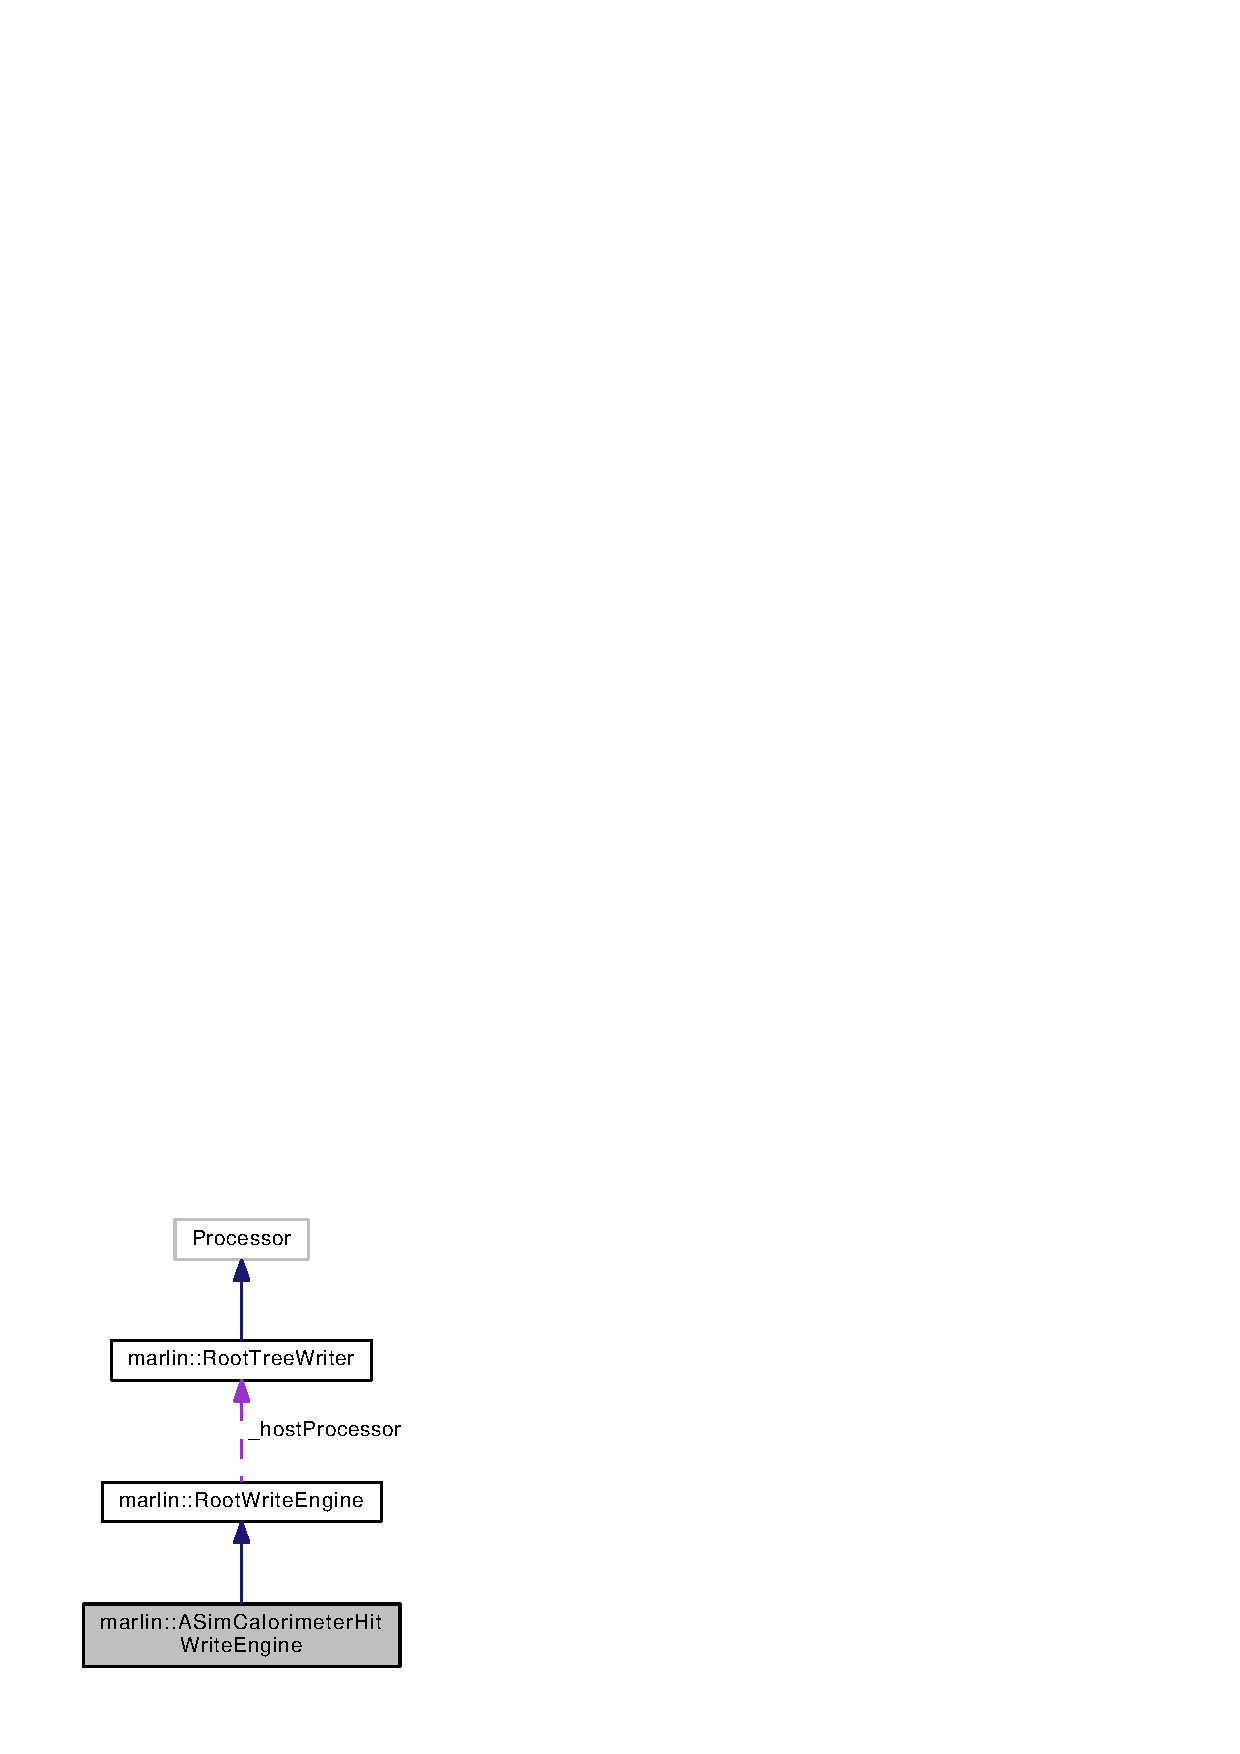
\includegraphics[width=197pt]{classmarlin_1_1ASimCalorimeterHitWriteEngine__coll__graph}
\end{center}
\end{figure}
\subsection*{Public Member Functions}
\begin{DoxyCompactItemize}
\item 
{\bfseries A\-Sim\-Calorimeter\-Hit\-Write\-Engine} ({\bf Root\-Tree\-Writer} $\ast$host)\label{classmarlin_1_1ASimCalorimeterHitWriteEngine_a752e10e04f17d7b292d9e90cf904ea18}

\item 
virtual const std\-::string \& {\bf get\-Engine\-Name} ()
\item 
virtual void {\bf register\-Parameters} ()
\item 
virtual void {\bf register\-Branches} (T\-Tree $\ast$host\-Tree)
\item 
virtual void {\bf fill\-Variables} (E\-V\-E\-N\-T\-::\-L\-C\-Event $\ast$)
\end{DoxyCompactItemize}
\subsection*{Additional Inherited Members}


\subsection{Detailed Description}


Definition at line 17 of file A\-Sim\-Calorimeter\-Hit\-Write\-Engine.\-hh.



\subsection{Member Function Documentation}
\index{marlin\-::\-A\-Sim\-Calorimeter\-Hit\-Write\-Engine@{marlin\-::\-A\-Sim\-Calorimeter\-Hit\-Write\-Engine}!fill\-Variables@{fill\-Variables}}
\index{fill\-Variables@{fill\-Variables}!marlin::ASimCalorimeterHitWriteEngine@{marlin\-::\-A\-Sim\-Calorimeter\-Hit\-Write\-Engine}}
\subsubsection[{fill\-Variables}]{\setlength{\rightskip}{0pt plus 5cm}void marlin\-::\-A\-Sim\-Calorimeter\-Hit\-Write\-Engine\-::fill\-Variables (
\begin{DoxyParamCaption}
\item[{E\-V\-E\-N\-T\-::\-L\-C\-Event $\ast$}]{evt}
\end{DoxyParamCaption}
)\hspace{0.3cm}{\ttfamily [virtual]}}\label{classmarlin_1_1ASimCalorimeterHitWriteEngine_a23a4c30ce18b277e5dc5150775633d12}
Implement this to extract the variables which you want to fill into the {\itshape R\-O\-O\-T} tree from the event. Write the value of the variables you want to add to the tree to the member variables, which you registered to the {\itshape R\-O\-O\-T} tree. The \doxyref{Root\-Tree\-Writer}{p.}{classmarlin_1_1RootTreeWriter} will call T\-Tree\-::\-Fill() for you. 
\begin{DoxyParams}{Parameters}
{\em evt} & the current event \\
\hline
\end{DoxyParams}


Implements {\bf marlin\-::\-Root\-Write\-Engine} \doxyref{}{p.}{classmarlin_1_1RootWriteEngine_ace823bd839cee7e8c8755e60c4cc7134}.



Definition at line 103 of file A\-Sim\-Calorimeter\-Hit\-Write\-Engine.\-cc.

\index{marlin\-::\-A\-Sim\-Calorimeter\-Hit\-Write\-Engine@{marlin\-::\-A\-Sim\-Calorimeter\-Hit\-Write\-Engine}!get\-Engine\-Name@{get\-Engine\-Name}}
\index{get\-Engine\-Name@{get\-Engine\-Name}!marlin::ASimCalorimeterHitWriteEngine@{marlin\-::\-A\-Sim\-Calorimeter\-Hit\-Write\-Engine}}
\subsubsection[{get\-Engine\-Name}]{\setlength{\rightskip}{0pt plus 5cm}virtual const std\-::string\& marlin\-::\-A\-Sim\-Calorimeter\-Hit\-Write\-Engine\-::get\-Engine\-Name (
\begin{DoxyParamCaption}
{}
\end{DoxyParamCaption}
)\hspace{0.3cm}{\ttfamily [inline]}, {\ttfamily [virtual]}}\label{classmarlin_1_1ASimCalorimeterHitWriteEngine_a76af2d1c30ce8566f1dcfacf551ab3dc}
Returns the name of the engine to the \doxyref{Root\-Tree\-Writer}{p.}{classmarlin_1_1RootTreeWriter} processor. \begin{DoxyReturn}{Returns}
Must return a string with the engine name. 
\end{DoxyReturn}
\begin{DoxyRefDesc}{Todo}
\item[{\bf Todo}]fixme\-: should be const, but must be declared const in implementations too. Need to fix all existing engines?!? \end{DoxyRefDesc}


Implements {\bf marlin\-::\-Root\-Write\-Engine} \doxyref{}{p.}{classmarlin_1_1RootWriteEngine_a31e38120fe60efcb15666fd569ba5862}.



Definition at line 75 of file A\-Sim\-Calorimeter\-Hit\-Write\-Engine.\-hh.

\index{marlin\-::\-A\-Sim\-Calorimeter\-Hit\-Write\-Engine@{marlin\-::\-A\-Sim\-Calorimeter\-Hit\-Write\-Engine}!register\-Branches@{register\-Branches}}
\index{register\-Branches@{register\-Branches}!marlin::ASimCalorimeterHitWriteEngine@{marlin\-::\-A\-Sim\-Calorimeter\-Hit\-Write\-Engine}}
\subsubsection[{register\-Branches}]{\setlength{\rightskip}{0pt plus 5cm}void marlin\-::\-A\-Sim\-Calorimeter\-Hit\-Write\-Engine\-::register\-Branches (
\begin{DoxyParamCaption}
\item[{T\-Tree $\ast$}]{}
\end{DoxyParamCaption}
)\hspace{0.3cm}{\ttfamily [virtual]}}\label{classmarlin_1_1ASimCalorimeterHitWriteEngine_a59a711512fa1cb7f0c3eb39a63af883d}
\begin{DoxyVerb}Implement to register local variables to the output tree
\param pointer to the \a ROOT tree, which the RootTreeWriter processor fills at the
end of each event.
Usually the implementation looks like@verbatim 
\end{DoxyVerb}
 /// host\-Tree-\/$>$Branch(\char`\"{}variable\char`\"{},\&\-\_\-variable\char`\"{} ,\char`\"{}variable/\-F" ); /// . But you can add any type of branch you like. 

Implements {\bf marlin\-::\-Root\-Write\-Engine} \doxyref{}{p.}{classmarlin_1_1RootWriteEngine_ad467dc6e73fdd9fd4311f7277fd02a89}.



Definition at line 45 of file A\-Sim\-Calorimeter\-Hit\-Write\-Engine.\-cc.

\index{marlin\-::\-A\-Sim\-Calorimeter\-Hit\-Write\-Engine@{marlin\-::\-A\-Sim\-Calorimeter\-Hit\-Write\-Engine}!register\-Parameters@{register\-Parameters}}
\index{register\-Parameters@{register\-Parameters}!marlin::ASimCalorimeterHitWriteEngine@{marlin\-::\-A\-Sim\-Calorimeter\-Hit\-Write\-Engine}}
\subsubsection[{register\-Parameters}]{\setlength{\rightskip}{0pt plus 5cm}void marlin\-::\-A\-Sim\-Calorimeter\-Hit\-Write\-Engine\-::register\-Parameters (
\begin{DoxyParamCaption}
{}
\end{DoxyParamCaption}
)\hspace{0.3cm}{\ttfamily [virtual]}}\label{classmarlin_1_1ASimCalorimeterHitWriteEngine_a5ad32bcf2f6723033b5a543a715f4d3c}
\begin{DoxyVerb}Used to register steering parameters.
Implement to register \a marlin steering file parameters. Use \a marlin syntax
to register parameters for the calling RootTreeWriter processor. 

use@verbatim 
\end{DoxyVerb}
 /// \-\_\-host\-Proc.\-relay\-Register\-Processor\-Parameter(...) /// \-\_\-host\-Proc.\-relay\-Register...() ///  instead of {\itshape marlin} processors\begin{DoxyVerb}register...() \end{DoxyVerb}
 methods 

Implements {\bf marlin\-::\-Root\-Write\-Engine} \doxyref{}{p.}{classmarlin_1_1RootWriteEngine_ae12b70923768043fa5c1438f078c41d3}.



Definition at line 26 of file A\-Sim\-Calorimeter\-Hit\-Write\-Engine.\-cc.



The documentation for this class was generated from the following files\-:\begin{DoxyCompactItemize}
\item 
A\-Sim\-Calorimeter\-Hit\-Write\-Engine.\-hh\item 
A\-Sim\-Calorimeter\-Hit\-Write\-Engine.\-cc\end{DoxyCompactItemize}

\section{marlin\-:\-:Bif\-Write\-Engine Class Reference}
\label{classmarlin_1_1BifWriteEngine}\index{marlin\-::\-Bif\-Write\-Engine@{marlin\-::\-Bif\-Write\-Engine}}


Inheritance diagram for marlin\-:\-:Bif\-Write\-Engine\-:
\nopagebreak
\begin{figure}[H]
\begin{center}
\leavevmode
\includegraphics[width=178pt]{classmarlin_1_1BifWriteEngine__inherit__graph}
\end{center}
\end{figure}


Collaboration diagram for marlin\-:\-:Bif\-Write\-Engine\-:
\nopagebreak
\begin{figure}[H]
\begin{center}
\leavevmode
\includegraphics[width=188pt]{classmarlin_1_1BifWriteEngine__coll__graph}
\end{center}
\end{figure}
\subsection*{Public Member Functions}
\begin{DoxyCompactItemize}
\item 
{\bfseries Bif\-Write\-Engine} ({\bf Root\-Tree\-Writer} $\ast$host)\label{classmarlin_1_1BifWriteEngine_a393c8ffc9c727aa3cb6f110464a8a9c3}

\item 
virtual const std\-::string \& {\bf get\-Engine\-Name} ()
\item 
virtual void {\bf register\-Parameters} ()
\item 
virtual void {\bf register\-Branches} (T\-Tree $\ast$host\-Tree)
\item 
virtual void {\bf fill\-Variables} (E\-V\-E\-N\-T\-::\-L\-C\-Event $\ast$)
\end{DoxyCompactItemize}
\subsection*{Public Attributes}
\begin{DoxyCompactItemize}
\item 
\begin{tabbing}
xx\=xx\=xx\=xx\=xx\=xx\=xx\=xx\=xx\=\kill
struct \{\\
\>unsigned long long int {\bf StartAcq}\\
\>unsigned long long int {\bf StopAcq}\\
\>int {\bf nTrigger}\\
\>int {\bf source} [MAXTRIGGERS]\\
\>int {\bf BXID} [MAXTRIGGERS]\\
\>float {\bf Time} [MAXTRIGGERS]\\
\} {\bfseries \_bifFill}\label{classmarlin_1_1BifWriteEngine_acf18f6765f90f6dd9f948931c1f14cd6}
\\

\end{tabbing}\end{DoxyCompactItemize}
\subsection*{Static Public Attributes}
\begin{DoxyCompactItemize}
\item 
static const unsigned int {\bfseries M\-A\-X\-T\-R\-I\-G\-G\-E\-R\-S} = 100\label{classmarlin_1_1BifWriteEngine_ab2709146a56204c227071f925593d2ca}

\end{DoxyCompactItemize}
\subsection*{Additional Inherited Members}


\subsection{Detailed Description}


Definition at line 14 of file Bif\-Write\-Engine.\-hh.



\subsection{Member Function Documentation}
\index{marlin\-::\-Bif\-Write\-Engine@{marlin\-::\-Bif\-Write\-Engine}!fill\-Variables@{fill\-Variables}}
\index{fill\-Variables@{fill\-Variables}!marlin::BifWriteEngine@{marlin\-::\-Bif\-Write\-Engine}}
\subsubsection[{fill\-Variables}]{\setlength{\rightskip}{0pt plus 5cm}void marlin\-::\-Bif\-Write\-Engine\-::fill\-Variables (
\begin{DoxyParamCaption}
\item[{E\-V\-E\-N\-T\-::\-L\-C\-Event $\ast$}]{evt}
\end{DoxyParamCaption}
)\hspace{0.3cm}{\ttfamily [virtual]}}\label{classmarlin_1_1BifWriteEngine_a5945f044afb17e832cf63380d3aa4330}
Implement this to extract the variables which you want to fill into the {\itshape R\-O\-O\-T} tree from the event. Write the value of the variables you want to add to the tree to the member variables, which you registered to the {\itshape R\-O\-O\-T} tree. The \doxyref{Root\-Tree\-Writer}{p.}{classmarlin_1_1RootTreeWriter} will call T\-Tree\-::\-Fill() for you. 
\begin{DoxyParams}{Parameters}
{\em evt} & the current event \\
\hline
\end{DoxyParams}


Implements {\bf marlin\-::\-Root\-Write\-Engine} \doxyref{}{p.}{classmarlin_1_1RootWriteEngine_ace823bd839cee7e8c8755e60c4cc7134}.



Definition at line 78 of file Bif\-Write\-Engine.\-cc.

\index{marlin\-::\-Bif\-Write\-Engine@{marlin\-::\-Bif\-Write\-Engine}!get\-Engine\-Name@{get\-Engine\-Name}}
\index{get\-Engine\-Name@{get\-Engine\-Name}!marlin::BifWriteEngine@{marlin\-::\-Bif\-Write\-Engine}}
\subsubsection[{get\-Engine\-Name}]{\setlength{\rightskip}{0pt plus 5cm}virtual const std\-::string\& marlin\-::\-Bif\-Write\-Engine\-::get\-Engine\-Name (
\begin{DoxyParamCaption}
{}
\end{DoxyParamCaption}
)\hspace{0.3cm}{\ttfamily [inline]}, {\ttfamily [virtual]}}\label{classmarlin_1_1BifWriteEngine_a82eecc72c7824876b9bb6211d9055e68}
Returns the name of the engine to the \doxyref{Root\-Tree\-Writer}{p.}{classmarlin_1_1RootTreeWriter} processor. \begin{DoxyReturn}{Returns}
Must return a string with the engine name. 
\end{DoxyReturn}
\begin{DoxyRefDesc}{Todo}
\item[{\bf Todo}]fixme\-: should be const, but must be declared const in implementations too. Need to fix all existing engines?!? \end{DoxyRefDesc}


Implements {\bf marlin\-::\-Root\-Write\-Engine} \doxyref{}{p.}{classmarlin_1_1RootWriteEngine_a31e38120fe60efcb15666fd569ba5862}.



Definition at line 23 of file Bif\-Write\-Engine.\-hh.

\index{marlin\-::\-Bif\-Write\-Engine@{marlin\-::\-Bif\-Write\-Engine}!register\-Branches@{register\-Branches}}
\index{register\-Branches@{register\-Branches}!marlin::BifWriteEngine@{marlin\-::\-Bif\-Write\-Engine}}
\subsubsection[{register\-Branches}]{\setlength{\rightskip}{0pt plus 5cm}void marlin\-::\-Bif\-Write\-Engine\-::register\-Branches (
\begin{DoxyParamCaption}
\item[{T\-Tree $\ast$}]{}
\end{DoxyParamCaption}
)\hspace{0.3cm}{\ttfamily [virtual]}}\label{classmarlin_1_1BifWriteEngine_a7589d618bd6113f426333a1aede37855}
\begin{DoxyVerb}Implement to register local variables to the output tree
\param pointer to the \a ROOT tree, which the RootTreeWriter processor fills at the
end of each event.
Usually the implementation looks like@verbatim 
\end{DoxyVerb}
 /// host\-Tree-\/$>$Branch(\char`\"{}variable\char`\"{},\&\-\_\-variable\char`\"{} ,\char`\"{}variable/\-F" ); /// . But you can add any type of branch you like. 

Implements {\bf marlin\-::\-Root\-Write\-Engine} \doxyref{}{p.}{classmarlin_1_1RootWriteEngine_ad467dc6e73fdd9fd4311f7277fd02a89}.



Definition at line 52 of file Bif\-Write\-Engine.\-cc.

\index{marlin\-::\-Bif\-Write\-Engine@{marlin\-::\-Bif\-Write\-Engine}!register\-Parameters@{register\-Parameters}}
\index{register\-Parameters@{register\-Parameters}!marlin::BifWriteEngine@{marlin\-::\-Bif\-Write\-Engine}}
\subsubsection[{register\-Parameters}]{\setlength{\rightskip}{0pt plus 5cm}void marlin\-::\-Bif\-Write\-Engine\-::register\-Parameters (
\begin{DoxyParamCaption}
{}
\end{DoxyParamCaption}
)\hspace{0.3cm}{\ttfamily [virtual]}}\label{classmarlin_1_1BifWriteEngine_a2f0940793cbb3314fe21843f9bde321b}
\begin{DoxyVerb}Used to register steering parameters.
Implement to register \a marlin steering file parameters. Use \a marlin syntax
to register parameters for the calling RootTreeWriter processor. 

use@verbatim 
\end{DoxyVerb}
 /// \-\_\-host\-Proc.\-relay\-Register\-Processor\-Parameter(...) /// \-\_\-host\-Proc.\-relay\-Register...() ///  instead of {\itshape marlin} processors\begin{DoxyVerb}register...() \end{DoxyVerb}
 methods 

Implements {\bf marlin\-::\-Root\-Write\-Engine} \doxyref{}{p.}{classmarlin_1_1RootWriteEngine_ae12b70923768043fa5c1438f078c41d3}.



Definition at line 33 of file Bif\-Write\-Engine.\-cc.



\subsection{Member Data Documentation}
\index{marlin\-::\-Bif\-Write\-Engine@{marlin\-::\-Bif\-Write\-Engine}!B\-X\-I\-D@{B\-X\-I\-D}}
\index{B\-X\-I\-D@{B\-X\-I\-D}!marlin::BifWriteEngine@{marlin\-::\-Bif\-Write\-Engine}}
\subsubsection[{B\-X\-I\-D}]{\setlength{\rightskip}{0pt plus 5cm}int marlin\-::\-Bif\-Write\-Engine\-::\-B\-X\-I\-D[M\-A\-X\-T\-R\-I\-G\-G\-E\-R\-S]}\label{classmarlin_1_1BifWriteEngine_ac35e4dfa1bf05cab9765ffd83580599c}
B\-X\-I\-D of the Trigger 

Definition at line 40 of file Bif\-Write\-Engine.\-hh.

\index{marlin\-::\-Bif\-Write\-Engine@{marlin\-::\-Bif\-Write\-Engine}!n\-Trigger@{n\-Trigger}}
\index{n\-Trigger@{n\-Trigger}!marlin::BifWriteEngine@{marlin\-::\-Bif\-Write\-Engine}}
\subsubsection[{n\-Trigger}]{\setlength{\rightskip}{0pt plus 5cm}int marlin\-::\-Bif\-Write\-Engine\-::n\-Trigger}\label{classmarlin_1_1BifWriteEngine_aa356c9b06febd7f97ab0bf0fe41462aa}
Number of B\-I\-F Triggers 

Definition at line 38 of file Bif\-Write\-Engine.\-hh.

\index{marlin\-::\-Bif\-Write\-Engine@{marlin\-::\-Bif\-Write\-Engine}!source@{source}}
\index{source@{source}!marlin::BifWriteEngine@{marlin\-::\-Bif\-Write\-Engine}}
\subsubsection[{source}]{\setlength{\rightskip}{0pt plus 5cm}int marlin\-::\-Bif\-Write\-Engine\-::source[M\-A\-X\-T\-R\-I\-G\-G\-E\-R\-S]}\label{classmarlin_1_1BifWriteEngine_a96e76f33457ffcd263fe36f8b5756c57}
Source of the Trigger (3 for Scint) 

Definition at line 39 of file Bif\-Write\-Engine.\-hh.

\index{marlin\-::\-Bif\-Write\-Engine@{marlin\-::\-Bif\-Write\-Engine}!Start\-Acq@{Start\-Acq}}
\index{Start\-Acq@{Start\-Acq}!marlin::BifWriteEngine@{marlin\-::\-Bif\-Write\-Engine}}
\subsubsection[{Start\-Acq}]{\setlength{\rightskip}{0pt plus 5cm}unsigned long long int marlin\-::\-Bif\-Write\-Engine\-::\-Start\-Acq}\label{classmarlin_1_1BifWriteEngine_a18fc0ff0830989602c485b8004af0c93}
Timestamp of the start acquisition 

Definition at line 36 of file Bif\-Write\-Engine.\-hh.

\index{marlin\-::\-Bif\-Write\-Engine@{marlin\-::\-Bif\-Write\-Engine}!Stop\-Acq@{Stop\-Acq}}
\index{Stop\-Acq@{Stop\-Acq}!marlin::BifWriteEngine@{marlin\-::\-Bif\-Write\-Engine}}
\subsubsection[{Stop\-Acq}]{\setlength{\rightskip}{0pt plus 5cm}unsigned long long int marlin\-::\-Bif\-Write\-Engine\-::\-Stop\-Acq}\label{classmarlin_1_1BifWriteEngine_ad65a5caebe02d633119beb5ffda2d49c}
Timestamp of the stop acquisition 

Definition at line 37 of file Bif\-Write\-Engine.\-hh.

\index{marlin\-::\-Bif\-Write\-Engine@{marlin\-::\-Bif\-Write\-Engine}!Time@{Time}}
\index{Time@{Time}!marlin::BifWriteEngine@{marlin\-::\-Bif\-Write\-Engine}}
\subsubsection[{Time}]{\setlength{\rightskip}{0pt plus 5cm}float marlin\-::\-Bif\-Write\-Engine\-::\-Time[M\-A\-X\-T\-R\-I\-G\-G\-E\-R\-S]}\label{classmarlin_1_1BifWriteEngine_a01b22dcf9615629cfa81794edb24f366}
Absolute Time of the Trigger 

Definition at line 41 of file Bif\-Write\-Engine.\-hh.



The documentation for this class was generated from the following files\-:\begin{DoxyCompactItemize}
\item 
Bif\-Write\-Engine.\-hh\item 
Bif\-Write\-Engine.\-cc\end{DoxyCompactItemize}

\section{marlin\-:\-:Collection\-Parameter\-Write\-Engine Class Reference}
\label{classmarlin_1_1CollectionParameterWriteEngine}\index{marlin\-::\-Collection\-Parameter\-Write\-Engine@{marlin\-::\-Collection\-Parameter\-Write\-Engine}}


Inheritance diagram for marlin\-:\-:Collection\-Parameter\-Write\-Engine\-:
\nopagebreak
\begin{figure}[H]
\begin{center}
\leavevmode
\includegraphics[width=196pt]{classmarlin_1_1CollectionParameterWriteEngine__inherit__graph}
\end{center}
\end{figure}


Collaboration diagram for marlin\-:\-:Collection\-Parameter\-Write\-Engine\-:
\nopagebreak
\begin{figure}[H]
\begin{center}
\leavevmode
\includegraphics[width=197pt]{classmarlin_1_1CollectionParameterWriteEngine__coll__graph}
\end{center}
\end{figure}
\subsection*{Public Member Functions}
\begin{DoxyCompactItemize}
\item 
{\bfseries Collection\-Parameter\-Write\-Engine} ({\bf Root\-Tree\-Writer} $\ast$host, std\-::string engine\-Name=\char`\"{}Collection\-Parameter\-Write\-Engine\char`\"{})\label{classmarlin_1_1CollectionParameterWriteEngine_af20b067194c5cbb2736c03eef94eeaa2}

\item 
virtual const std\-::string \& {\bf get\-Engine\-Name} ()
\item 
virtual void {\bf register\-Parameters} ()
\item 
virtual void {\bf register\-Branches} (T\-Tree $\ast$host\-Tree)
\item 
virtual void {\bf fill\-Variables} (E\-V\-E\-N\-T\-::\-L\-C\-Event $\ast$)
\end{DoxyCompactItemize}
\subsection*{Public Attributes}
\begin{DoxyCompactItemize}
\item 
std\-::vector$<$ int $>$ {\bfseries \-\_\-int\-Values}\label{classmarlin_1_1CollectionParameterWriteEngine_aabaea90c0dddbe134a72a30bf4e83d41}

\item 
std\-::vector$<$ float $>$ {\bfseries \-\_\-float\-Values}\label{classmarlin_1_1CollectionParameterWriteEngine_ac4e123e59a02a486115299feeeca1625}

\item 
std\-::vector$<$ Int\-Vec $>$ {\bfseries \-\_\-int\-Vec\-Values}\label{classmarlin_1_1CollectionParameterWriteEngine_ad85958fa647d7838c4087bbdc55bf08e}

\item 
std\-::vector$<$ Float\-Vec $>$ {\bfseries \-\_\-float\-Vec\-Values}\label{classmarlin_1_1CollectionParameterWriteEngine_a94805eac93affa52fd2aeb7d40a961b4}

\item 
std\-::vector$<$ int $>$ {\bfseries \-\_\-n\-Int\-Values}\label{classmarlin_1_1CollectionParameterWriteEngine_a85921dba71a30b3a97e2706c876e460e}

\item 
std\-::vector$<$ int $>$ {\bfseries \-\_\-n\-Float\-Values}\label{classmarlin_1_1CollectionParameterWriteEngine_a11064e5166350ef8c3b60c4334edb05c}

\end{DoxyCompactItemize}
\subsection*{Additional Inherited Members}


\subsection{Detailed Description}


Definition at line 16 of file Collection\-Parameter\-Write\-Engine.\-hh.



\subsection{Member Function Documentation}
\index{marlin\-::\-Collection\-Parameter\-Write\-Engine@{marlin\-::\-Collection\-Parameter\-Write\-Engine}!fill\-Variables@{fill\-Variables}}
\index{fill\-Variables@{fill\-Variables}!marlin::CollectionParameterWriteEngine@{marlin\-::\-Collection\-Parameter\-Write\-Engine}}
\subsubsection[{fill\-Variables}]{\setlength{\rightskip}{0pt plus 5cm}void marlin\-::\-Collection\-Parameter\-Write\-Engine\-::fill\-Variables (
\begin{DoxyParamCaption}
\item[{E\-V\-E\-N\-T\-::\-L\-C\-Event $\ast$}]{evt}
\end{DoxyParamCaption}
)\hspace{0.3cm}{\ttfamily [virtual]}}\label{classmarlin_1_1CollectionParameterWriteEngine_a276cbc4b3fb6a51d52b7ff677cbe60ad}
Implement this to extract the variables which you want to fill into the {\itshape R\-O\-O\-T} tree from the event. Write the value of the variables you want to add to the tree to the member variables, which you registered to the {\itshape R\-O\-O\-T} tree. The \doxyref{Root\-Tree\-Writer}{p.}{classmarlin_1_1RootTreeWriter} will call T\-Tree\-::\-Fill() for you. 
\begin{DoxyParams}{Parameters}
{\em evt} & the current event \\
\hline
\end{DoxyParams}


Implements {\bf marlin\-::\-Root\-Write\-Engine} \doxyref{}{p.}{classmarlin_1_1RootWriteEngine_ace823bd839cee7e8c8755e60c4cc7134}.



Definition at line 88 of file Collection\-Parameter\-Write\-Engine.\-cc.

\index{marlin\-::\-Collection\-Parameter\-Write\-Engine@{marlin\-::\-Collection\-Parameter\-Write\-Engine}!get\-Engine\-Name@{get\-Engine\-Name}}
\index{get\-Engine\-Name@{get\-Engine\-Name}!marlin::CollectionParameterWriteEngine@{marlin\-::\-Collection\-Parameter\-Write\-Engine}}
\subsubsection[{get\-Engine\-Name}]{\setlength{\rightskip}{0pt plus 5cm}virtual const std\-::string\& marlin\-::\-Collection\-Parameter\-Write\-Engine\-::get\-Engine\-Name (
\begin{DoxyParamCaption}
{}
\end{DoxyParamCaption}
)\hspace{0.3cm}{\ttfamily [inline]}, {\ttfamily [virtual]}}\label{classmarlin_1_1CollectionParameterWriteEngine_aec77b9403ff1661fd01d714b433157e8}
Returns the name of the engine to the \doxyref{Root\-Tree\-Writer}{p.}{classmarlin_1_1RootTreeWriter} processor. \begin{DoxyReturn}{Returns}
Must return a string with the engine name. 
\end{DoxyReturn}
\begin{DoxyRefDesc}{Todo}
\item[{\bf Todo}]fixme\-: should be const, but must be declared const in implementations too. Need to fix all existing engines?!? \end{DoxyRefDesc}


Implements {\bf marlin\-::\-Root\-Write\-Engine} \doxyref{}{p.}{classmarlin_1_1RootWriteEngine_a31e38120fe60efcb15666fd569ba5862}.



Definition at line 24 of file Collection\-Parameter\-Write\-Engine.\-hh.

\index{marlin\-::\-Collection\-Parameter\-Write\-Engine@{marlin\-::\-Collection\-Parameter\-Write\-Engine}!register\-Branches@{register\-Branches}}
\index{register\-Branches@{register\-Branches}!marlin::CollectionParameterWriteEngine@{marlin\-::\-Collection\-Parameter\-Write\-Engine}}
\subsubsection[{register\-Branches}]{\setlength{\rightskip}{0pt plus 5cm}void marlin\-::\-Collection\-Parameter\-Write\-Engine\-::register\-Branches (
\begin{DoxyParamCaption}
\item[{T\-Tree $\ast$}]{}
\end{DoxyParamCaption}
)\hspace{0.3cm}{\ttfamily [virtual]}}\label{classmarlin_1_1CollectionParameterWriteEngine_afd2c829f35e899f90f881a37aef206f9}
\begin{DoxyVerb}Implement to register local variables to the output tree
\param pointer to the \a ROOT tree, which the RootTreeWriter processor fills at the
end of each event.
Usually the implementation looks like@verbatim 
\end{DoxyVerb}
 /// host\-Tree-\/$>$Branch(\char`\"{}variable\char`\"{},\&\-\_\-variable\char`\"{} ,\char`\"{}variable/\-F" ); /// . But you can add any type of branch you like. 

Implements {\bf marlin\-::\-Root\-Write\-Engine} \doxyref{}{p.}{classmarlin_1_1RootWriteEngine_ad467dc6e73fdd9fd4311f7277fd02a89}.



Definition at line 48 of file Collection\-Parameter\-Write\-Engine.\-cc.

\index{marlin\-::\-Collection\-Parameter\-Write\-Engine@{marlin\-::\-Collection\-Parameter\-Write\-Engine}!register\-Parameters@{register\-Parameters}}
\index{register\-Parameters@{register\-Parameters}!marlin::CollectionParameterWriteEngine@{marlin\-::\-Collection\-Parameter\-Write\-Engine}}
\subsubsection[{register\-Parameters}]{\setlength{\rightskip}{0pt plus 5cm}void marlin\-::\-Collection\-Parameter\-Write\-Engine\-::register\-Parameters (
\begin{DoxyParamCaption}
{}
\end{DoxyParamCaption}
)\hspace{0.3cm}{\ttfamily [virtual]}}\label{classmarlin_1_1CollectionParameterWriteEngine_ae5bd3085f961a8ecc90272f00886d7d8}
\begin{DoxyVerb}Used to register steering parameters.
Implement to register \a marlin steering file parameters. Use \a marlin syntax
to register parameters for the calling RootTreeWriter processor. 

use@verbatim 
\end{DoxyVerb}
 /// \-\_\-host\-Proc.\-relay\-Register\-Processor\-Parameter(...) /// \-\_\-host\-Proc.\-relay\-Register...() ///  instead of {\itshape marlin} processors\begin{DoxyVerb}register...() \end{DoxyVerb}
 methods 

Implements {\bf marlin\-::\-Root\-Write\-Engine} \doxyref{}{p.}{classmarlin_1_1RootWriteEngine_ae12b70923768043fa5c1438f078c41d3}.



Definition at line 20 of file Collection\-Parameter\-Write\-Engine.\-cc.



The documentation for this class was generated from the following files\-:\begin{DoxyCompactItemize}
\item 
Collection\-Parameter\-Write\-Engine.\-hh\item 
Collection\-Parameter\-Write\-Engine.\-cc\end{DoxyCompactItemize}

\section{\-\_\-\-\_\-\-R\-T\-W\-:\-:Compat\-Version\-Info Class Reference}
\label{class____RTW_1_1CompatVersionInfo}\index{\-\_\-\-\_\-\-R\-T\-W\-::\-Compat\-Version\-Info@{\-\_\-\-\_\-\-R\-T\-W\-::\-Compat\-Version\-Info}}


\subsection{Detailed Description}


Definition at line 22 of file Engine\-Registrar.\-hh.



The documentation for this class was generated from the following file\-:\begin{DoxyCompactItemize}
\item 
Engine\-Registrar.\-hh\end{DoxyCompactItemize}

\section{marlin\-:\-:Deep\-Ana\-Write\-Engine Class Reference}
\label{classmarlin_1_1DeepAnaWriteEngine}\index{marlin\-::\-Deep\-Ana\-Write\-Engine@{marlin\-::\-Deep\-Ana\-Write\-Engine}}


Inheritance diagram for marlin\-:\-:Deep\-Ana\-Write\-Engine\-:
\nopagebreak
\begin{figure}[H]
\begin{center}
\leavevmode
\includegraphics[width=200pt]{classmarlin_1_1DeepAnaWriteEngine__inherit__graph}
\end{center}
\end{figure}


Collaboration diagram for marlin\-:\-:Deep\-Ana\-Write\-Engine\-:
\nopagebreak
\begin{figure}[H]
\begin{center}
\leavevmode
\includegraphics[width=200pt]{classmarlin_1_1DeepAnaWriteEngine__coll__graph}
\end{center}
\end{figure}
\subsection*{Public Member Functions}
\begin{DoxyCompactItemize}
\item 
{\bfseries Deep\-Ana\-Write\-Engine} ({\bf Root\-Tree\-Writer} $\ast$host)\label{classmarlin_1_1DeepAnaWriteEngine_af7280abd120c35885bb82a45a78b9d32}

\item 
virtual const std\-::string \& {\bf get\-Engine\-Name} ()
\item 
virtual void {\bf register\-Parameters} ()
\item 
virtual void {\bf register\-Branches} (T\-Tree $\ast$host\-Tree)
\item 
virtual void {\bf fill\-Variables} (E\-V\-E\-N\-T\-::\-L\-C\-Event $\ast$)
\end{DoxyCompactItemize}
\subsection*{Public Attributes}
\begin{DoxyCompactItemize}
\item 
unsigned int {\bf \-\_\-elm\-No\-Clusters}\label{classmarlin_1_1DeepAnaWriteEngine_aca49605aaeaf9f8b1511c78a381e7c44}

\begin{DoxyCompactList}\small\item\em ! place the member variables to hold the R\-O\-O\-T T\-Tree branches here !!; \end{DoxyCompactList}\item 
unsigned int {\bfseries \-\_\-elm\-No\-Hits}\label{classmarlin_1_1DeepAnaWriteEngine_a26993881ac5d2e9b855fba85d7ea208a}

\item 
double {\bfseries \-\_\-elm\-Engy\-Sum}\label{classmarlin_1_1DeepAnaWriteEngine_aa7d28857da02a8d2b429f5955914669d}

\item 
unsigned int {\bfseries \-\_\-trk\-No\-Clusters}\label{classmarlin_1_1DeepAnaWriteEngine_a1abca1be5b1ca9d7e7db53a41af4e127}

\item 
unsigned int {\bfseries \-\_\-trk\-No\-Hits}\label{classmarlin_1_1DeepAnaWriteEngine_afd2268ec39b86bf356c99fa0cf687915}

\item 
double {\bfseries \-\_\-trk\-Engy\-Sum}\label{classmarlin_1_1DeepAnaWriteEngine_ae3de8e96baa3464c5b485ca606009c30}

\item 
unsigned int {\bfseries \-\_\-had\-No\-Clusters}\label{classmarlin_1_1DeepAnaWriteEngine_a02ffeaed8c9e41740adcf22d09500386}

\item 
unsigned int {\bfseries \-\_\-had\-No\-Hits}\label{classmarlin_1_1DeepAnaWriteEngine_ae297a6c2d2faf5e172ac9261c0ef0348}

\item 
double {\bfseries \-\_\-had\-Engy\-Sum}\label{classmarlin_1_1DeepAnaWriteEngine_ae072724fa8177f7f20712dead1e1bbb8}

\item 
unsigned int {\bfseries \-\_\-neutr\-No\-Hits}\label{classmarlin_1_1DeepAnaWriteEngine_a0faa79a58bc077840c396f613984dc25}

\item 
double {\bfseries \-\_\-neutr\-Engy\-Sum}\label{classmarlin_1_1DeepAnaWriteEngine_a52d8f316284e964036931b1c8c52c73a}

\item 
double {\bfseries \-\_\-elm\-X}\label{classmarlin_1_1DeepAnaWriteEngine_aa0217dcc3006f49410d4f7ad9caa689b}

\item 
double {\bfseries \-\_\-elm\-Y}\label{classmarlin_1_1DeepAnaWriteEngine_a977967fe6dfc9ba6f6fb5a3c6eb0b7cd}

\item 
double {\bfseries \-\_\-elm\-Z}\label{classmarlin_1_1DeepAnaWriteEngine_ae2459fc29b2a4545bb990911b131d469}

\item 
double {\bfseries \-\_\-trk\-X}\label{classmarlin_1_1DeepAnaWriteEngine_a80b166fb03c427a92b8f5fa202f696b9}

\item 
double {\bfseries \-\_\-trk\-Y}\label{classmarlin_1_1DeepAnaWriteEngine_a35808f0e2b6100117f52d7e85406ad69}

\item 
double {\bfseries \-\_\-trk\-Z}\label{classmarlin_1_1DeepAnaWriteEngine_ac9bac299dd35b8129c088f6c7a6ad135}

\item 
double {\bfseries \-\_\-had\-X}\label{classmarlin_1_1DeepAnaWriteEngine_adcf35e54d9321c7e1cb026de6d33aec6}

\item 
double {\bfseries \-\_\-had\-Y}\label{classmarlin_1_1DeepAnaWriteEngine_aab5db65045f127924788f62c504275bb}

\item 
double {\bfseries \-\_\-had\-Z}\label{classmarlin_1_1DeepAnaWriteEngine_a84830c7ba3ad4928bb25795f5adde6f4}

\item 
double {\bfseries \-\_\-\-X}\label{classmarlin_1_1DeepAnaWriteEngine_a622e86e7f0d2614e26771aea8c692e66}

\item 
double {\bfseries \-\_\-\-Y}\label{classmarlin_1_1DeepAnaWriteEngine_a74dc25aac2fb941dd2121c1b22ef689e}

\item 
double {\bfseries \-\_\-\-Z}\label{classmarlin_1_1DeepAnaWriteEngine_a38610d44a5c8a783a27862e63b22f55b}

\end{DoxyCompactItemize}
\subsection*{Additional Inherited Members}


\subsection{Detailed Description}


Definition at line 16 of file Deep\-Ana\-Write\-Engine.\-hh.



\subsection{Member Function Documentation}
\index{marlin\-::\-Deep\-Ana\-Write\-Engine@{marlin\-::\-Deep\-Ana\-Write\-Engine}!fill\-Variables@{fill\-Variables}}
\index{fill\-Variables@{fill\-Variables}!marlin::DeepAnaWriteEngine@{marlin\-::\-Deep\-Ana\-Write\-Engine}}
\subsubsection[{fill\-Variables}]{\setlength{\rightskip}{0pt plus 5cm}virtual void marlin\-::\-Deep\-Ana\-Write\-Engine\-::fill\-Variables (
\begin{DoxyParamCaption}
\item[{E\-V\-E\-N\-T\-::\-L\-C\-Event $\ast$}]{evt}
\end{DoxyParamCaption}
)\hspace{0.3cm}{\ttfamily [virtual]}}\label{classmarlin_1_1DeepAnaWriteEngine_a9cf77605dc60b01d00169c80c2df921d}
Implement this to extract the variables which you want to fill into the {\itshape R\-O\-O\-T} tree from the event. Write the value of the variables you want to add to the tree to the member variables, which you registered to the {\itshape R\-O\-O\-T} tree. The \doxyref{Root\-Tree\-Writer}{p.}{classmarlin_1_1RootTreeWriter} will call T\-Tree\-::\-Fill() for you. 
\begin{DoxyParams}{Parameters}
{\em evt} & the current event \\
\hline
\end{DoxyParams}


Implements {\bf marlin\-::\-Root\-Write\-Engine} \doxyref{}{p.}{classmarlin_1_1RootWriteEngine_ace823bd839cee7e8c8755e60c4cc7134}.

\index{marlin\-::\-Deep\-Ana\-Write\-Engine@{marlin\-::\-Deep\-Ana\-Write\-Engine}!get\-Engine\-Name@{get\-Engine\-Name}}
\index{get\-Engine\-Name@{get\-Engine\-Name}!marlin::DeepAnaWriteEngine@{marlin\-::\-Deep\-Ana\-Write\-Engine}}
\subsubsection[{get\-Engine\-Name}]{\setlength{\rightskip}{0pt plus 5cm}virtual const std\-::string\& marlin\-::\-Deep\-Ana\-Write\-Engine\-::get\-Engine\-Name (
\begin{DoxyParamCaption}
{}
\end{DoxyParamCaption}
)\hspace{0.3cm}{\ttfamily [inline]}, {\ttfamily [virtual]}}\label{classmarlin_1_1DeepAnaWriteEngine_a3b67cb94563a6f930a28f71bba8833c1}
Returns the name of the engine to the \doxyref{Root\-Tree\-Writer}{p.}{classmarlin_1_1RootTreeWriter} processor. \begin{DoxyReturn}{Returns}
Must return a string with the engine name. 
\end{DoxyReturn}
\begin{DoxyRefDesc}{Todo}
\item[{\bf Todo}]fixme\-: should be const, but must be declared const in implementations too. Need to fix all existing engines?!? \end{DoxyRefDesc}


Implements {\bf marlin\-::\-Root\-Write\-Engine} \doxyref{}{p.}{classmarlin_1_1RootWriteEngine_a31e38120fe60efcb15666fd569ba5862}.



Definition at line 25 of file Deep\-Ana\-Write\-Engine.\-hh.

\index{marlin\-::\-Deep\-Ana\-Write\-Engine@{marlin\-::\-Deep\-Ana\-Write\-Engine}!register\-Branches@{register\-Branches}}
\index{register\-Branches@{register\-Branches}!marlin::DeepAnaWriteEngine@{marlin\-::\-Deep\-Ana\-Write\-Engine}}
\subsubsection[{register\-Branches}]{\setlength{\rightskip}{0pt plus 5cm}virtual void marlin\-::\-Deep\-Ana\-Write\-Engine\-::register\-Branches (
\begin{DoxyParamCaption}
\item[{T\-Tree $\ast$}]{}
\end{DoxyParamCaption}
)\hspace{0.3cm}{\ttfamily [virtual]}}\label{classmarlin_1_1DeepAnaWriteEngine_afa0d65f082b588ef7d61c06aecd9afe4}
\begin{DoxyVerb}Implement to register local variables to the output tree
\param pointer to the \a ROOT tree, which the RootTreeWriter processor fills at the
end of each event.
Usually the implementation looks like@verbatim 
\end{DoxyVerb}
 /// host\-Tree-\/$>$Branch(\char`\"{}variable\char`\"{},\&\-\_\-variable\char`\"{} ,\char`\"{}variable/\-F" ); /// . But you can add any type of branch you like. 

Implements {\bf marlin\-::\-Root\-Write\-Engine} \doxyref{}{p.}{classmarlin_1_1RootWriteEngine_ad467dc6e73fdd9fd4311f7277fd02a89}.

\index{marlin\-::\-Deep\-Ana\-Write\-Engine@{marlin\-::\-Deep\-Ana\-Write\-Engine}!register\-Parameters@{register\-Parameters}}
\index{register\-Parameters@{register\-Parameters}!marlin::DeepAnaWriteEngine@{marlin\-::\-Deep\-Ana\-Write\-Engine}}
\subsubsection[{register\-Parameters}]{\setlength{\rightskip}{0pt plus 5cm}virtual void marlin\-::\-Deep\-Ana\-Write\-Engine\-::register\-Parameters (
\begin{DoxyParamCaption}
{}
\end{DoxyParamCaption}
)\hspace{0.3cm}{\ttfamily [virtual]}}\label{classmarlin_1_1DeepAnaWriteEngine_a757be550fb07212cfbe8cd2a9d6e26be}
\begin{DoxyVerb}Used to register steering parameters.
Implement to register \a marlin steering file parameters. Use \a marlin syntax
to register parameters for the calling RootTreeWriter processor. 

use@verbatim 
\end{DoxyVerb}
 /// \-\_\-host\-Proc.\-relay\-Register\-Processor\-Parameter(...) /// \-\_\-host\-Proc.\-relay\-Register...() ///  instead of {\itshape marlin} processors\begin{DoxyVerb}register...() \end{DoxyVerb}
 methods 

Implements {\bf marlin\-::\-Root\-Write\-Engine} \doxyref{}{p.}{classmarlin_1_1RootWriteEngine_ae12b70923768043fa5c1438f078c41d3}.



The documentation for this class was generated from the following file\-:\begin{DoxyCompactItemize}
\item 
Deep\-Ana\-Write\-Engine.\-hh\end{DoxyCompactItemize}

\section{marlin\-:\-:Drift\-Chamber\-Write\-Engine Class Reference}
\label{classmarlin_1_1DriftChamberWriteEngine}\index{marlin\-::\-Drift\-Chamber\-Write\-Engine@{marlin\-::\-Drift\-Chamber\-Write\-Engine}}


Inheritance diagram for marlin\-:\-:Drift\-Chamber\-Write\-Engine\-:
\nopagebreak
\begin{figure}[H]
\begin{center}
\leavevmode
\includegraphics[width=190pt]{classmarlin_1_1DriftChamberWriteEngine__inherit__graph}
\end{center}
\end{figure}


Collaboration diagram for marlin\-:\-:Drift\-Chamber\-Write\-Engine\-:
\nopagebreak
\begin{figure}[H]
\begin{center}
\leavevmode
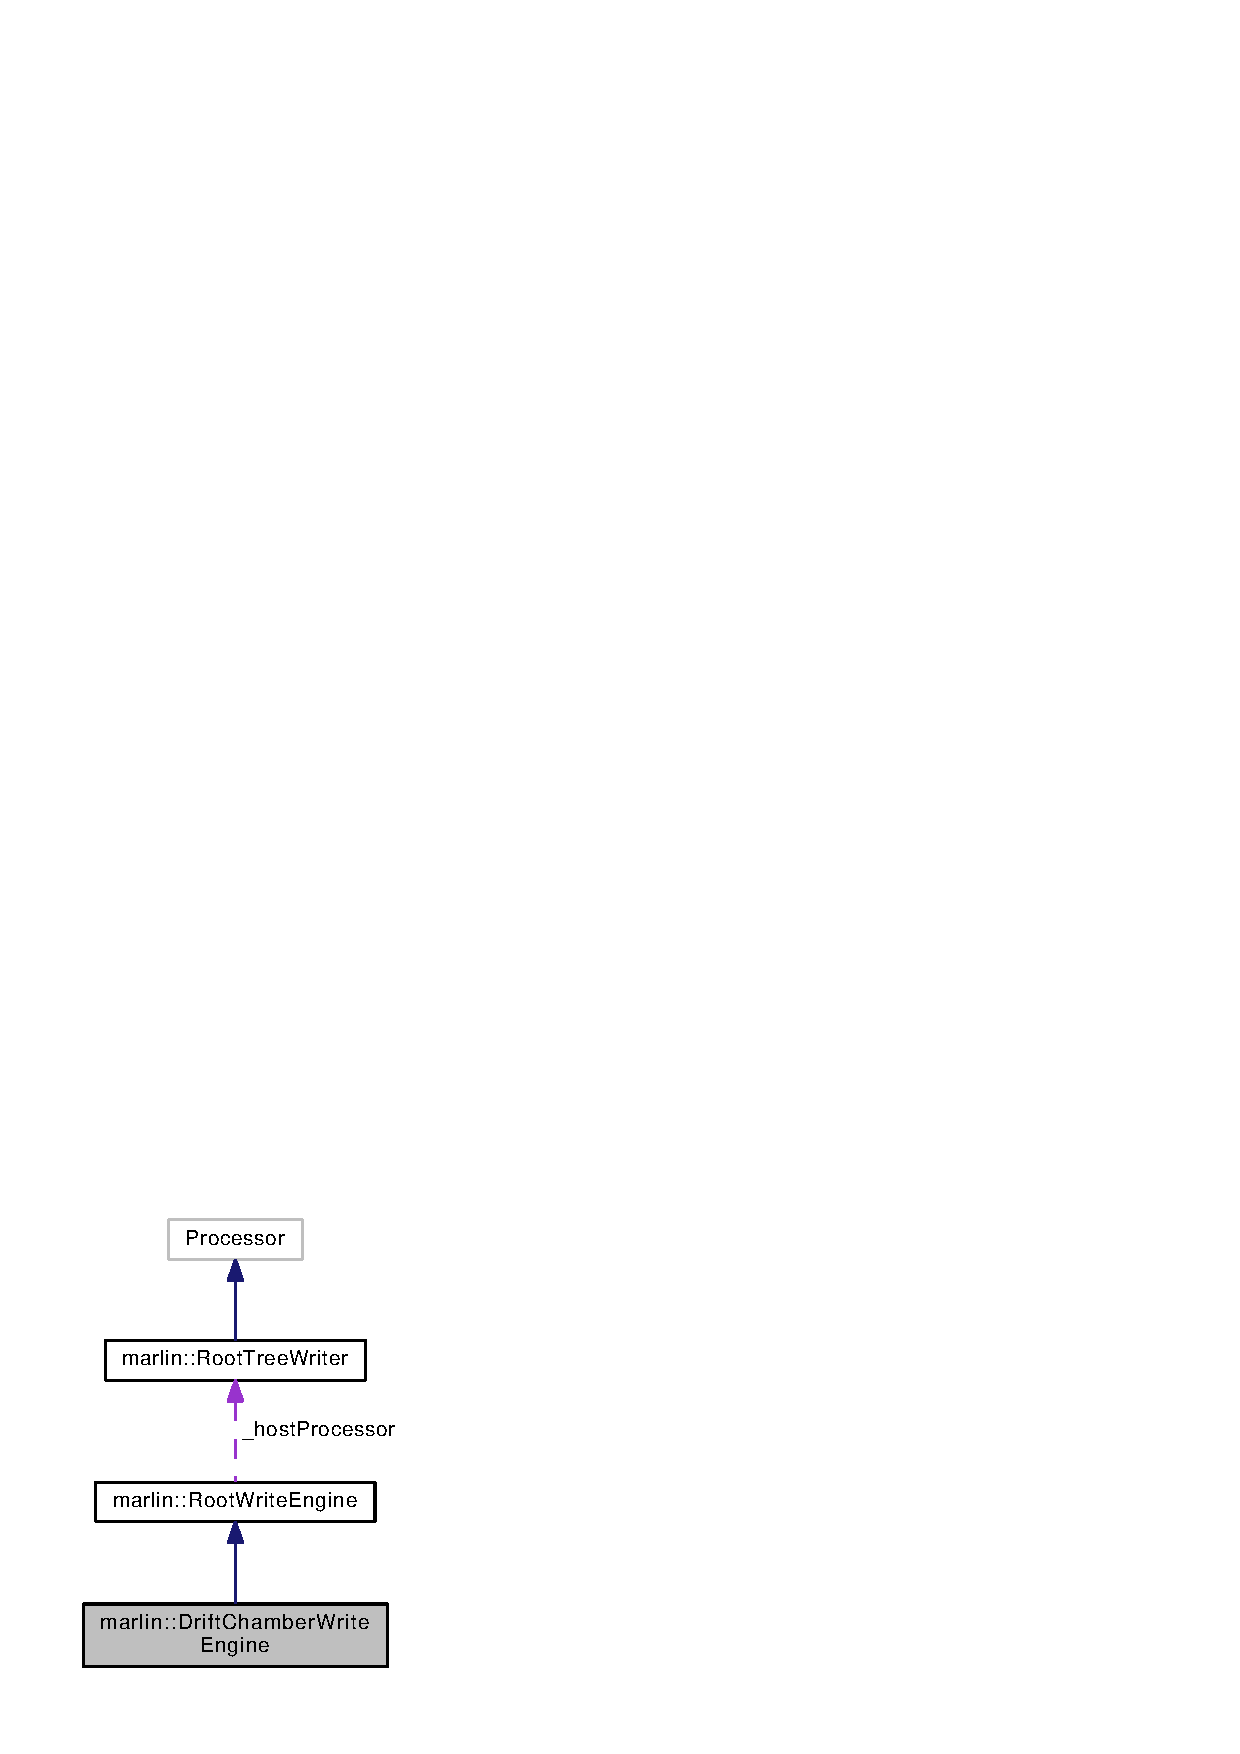
\includegraphics[width=194pt]{classmarlin_1_1DriftChamberWriteEngine__coll__graph}
\end{center}
\end{figure}
\subsection*{Public Member Functions}
\begin{DoxyCompactItemize}
\item 
{\bfseries Drift\-Chamber\-Write\-Engine} ({\bf Root\-Tree\-Writer} $\ast$host)\label{classmarlin_1_1DriftChamberWriteEngine_a2650f5a2c8e56d670f8ffd2f9ae6d872}

\item 
virtual const std\-::string \& {\bf get\-Engine\-Name} ()
\item 
virtual void {\bf register\-Parameters} ()
\item 
virtual void {\bf register\-Branches} (T\-Tree $\ast$host\-Tree)
\item 
virtual void {\bf fill\-Variables} (E\-V\-E\-N\-T\-::\-L\-C\-Event $\ast$)
\end{DoxyCompactItemize}
\subsection*{Public Attributes}
\begin{DoxyCompactItemize}
\item 
\begin{tabbing}
xx\=xx\=xx\=xx\=xx\=xx\=xx\=xx\=xx\=\kill
struct \{\\
\>float {\bfseries EcalXYZ} [3]\\
\>float {\bfseries HcalXYZ} [3]\\
\>float {\bfseries Phi}\\
\>float {\bfseries Lambda}\\
\>float {\bfseries Chi2}\\
\} {\bfseries \_hitsFill}\label{classmarlin_1_1DriftChamberWriteEngine_a6b016c299ff4d1537ade6592c45303f5}
\\

\end{tabbing}\end{DoxyCompactItemize}
\subsection*{Static Public Attributes}
\begin{DoxyCompactItemize}
\item 
static const unsigned int {\bfseries M\-A\-X\-H\-I\-T\-S} = 7608\label{classmarlin_1_1DriftChamberWriteEngine_af0a61ec798ac8419a1aba09bc9d35a68}

\end{DoxyCompactItemize}
\subsection*{Additional Inherited Members}


\subsection{Detailed Description}


Definition at line 17 of file Drift\-Chamber\-Write\-Engine.\-hh.



\subsection{Member Function Documentation}
\index{marlin\-::\-Drift\-Chamber\-Write\-Engine@{marlin\-::\-Drift\-Chamber\-Write\-Engine}!fill\-Variables@{fill\-Variables}}
\index{fill\-Variables@{fill\-Variables}!marlin::DriftChamberWriteEngine@{marlin\-::\-Drift\-Chamber\-Write\-Engine}}
\subsubsection[{fill\-Variables}]{\setlength{\rightskip}{0pt plus 5cm}void marlin\-::\-Drift\-Chamber\-Write\-Engine\-::fill\-Variables (
\begin{DoxyParamCaption}
\item[{E\-V\-E\-N\-T\-::\-L\-C\-Event $\ast$}]{evt}
\end{DoxyParamCaption}
)\hspace{0.3cm}{\ttfamily [virtual]}}\label{classmarlin_1_1DriftChamberWriteEngine_ae4ac9d60684437fd6b4d5c3365c0e7ef}
Implement this to extract the variables which you want to fill into the {\itshape R\-O\-O\-T} tree from the event. Write the value of the variables you want to add to the tree to the member variables, which you registered to the {\itshape R\-O\-O\-T} tree. The \doxyref{Root\-Tree\-Writer}{p.}{classmarlin_1_1RootTreeWriter} will call T\-Tree\-::\-Fill() for you. 
\begin{DoxyParams}{Parameters}
{\em evt} & the current event \\
\hline
\end{DoxyParams}


Implements {\bf marlin\-::\-Root\-Write\-Engine} \doxyref{}{p.}{classmarlin_1_1RootWriteEngine_ace823bd839cee7e8c8755e60c4cc7134}.



Definition at line 47 of file Drift\-Chamber\-Write\-Engine.\-cc.

\index{marlin\-::\-Drift\-Chamber\-Write\-Engine@{marlin\-::\-Drift\-Chamber\-Write\-Engine}!get\-Engine\-Name@{get\-Engine\-Name}}
\index{get\-Engine\-Name@{get\-Engine\-Name}!marlin::DriftChamberWriteEngine@{marlin\-::\-Drift\-Chamber\-Write\-Engine}}
\subsubsection[{get\-Engine\-Name}]{\setlength{\rightskip}{0pt plus 5cm}virtual const std\-::string\& marlin\-::\-Drift\-Chamber\-Write\-Engine\-::get\-Engine\-Name (
\begin{DoxyParamCaption}
{}
\end{DoxyParamCaption}
)\hspace{0.3cm}{\ttfamily [inline]}, {\ttfamily [virtual]}}\label{classmarlin_1_1DriftChamberWriteEngine_a54c3c6b481d7f957c95dc0b8dd9b9d37}
Returns the name of the engine to the \doxyref{Root\-Tree\-Writer}{p.}{classmarlin_1_1RootTreeWriter} processor. \begin{DoxyReturn}{Returns}
Must return a string with the engine name. 
\end{DoxyReturn}
\begin{DoxyRefDesc}{Todo}
\item[{\bf Todo}]fixme\-: should be const, but must be declared const in implementations too. Need to fix all existing engines?!? \end{DoxyRefDesc}


Implements {\bf marlin\-::\-Root\-Write\-Engine} \doxyref{}{p.}{classmarlin_1_1RootWriteEngine_a31e38120fe60efcb15666fd569ba5862}.



Definition at line 26 of file Drift\-Chamber\-Write\-Engine.\-hh.

\index{marlin\-::\-Drift\-Chamber\-Write\-Engine@{marlin\-::\-Drift\-Chamber\-Write\-Engine}!register\-Branches@{register\-Branches}}
\index{register\-Branches@{register\-Branches}!marlin::DriftChamberWriteEngine@{marlin\-::\-Drift\-Chamber\-Write\-Engine}}
\subsubsection[{register\-Branches}]{\setlength{\rightskip}{0pt plus 5cm}void marlin\-::\-Drift\-Chamber\-Write\-Engine\-::register\-Branches (
\begin{DoxyParamCaption}
\item[{T\-Tree $\ast$}]{}
\end{DoxyParamCaption}
)\hspace{0.3cm}{\ttfamily [virtual]}}\label{classmarlin_1_1DriftChamberWriteEngine_a3b32b9dc07adaa637821917ec5a879a3}
\begin{DoxyVerb}Implement to register local variables to the output tree
\param pointer to the \a ROOT tree, which the RootTreeWriter processor fills at the
end of each event.
Usually the implementation looks like@verbatim 
\end{DoxyVerb}
 /// host\-Tree-\/$>$Branch(\char`\"{}variable\char`\"{},\&\-\_\-variable\char`\"{} ,\char`\"{}variable/\-F" ); /// . But you can add any type of branch you like. 

Implements {\bf marlin\-::\-Root\-Write\-Engine} \doxyref{}{p.}{classmarlin_1_1RootWriteEngine_ad467dc6e73fdd9fd4311f7277fd02a89}.



Definition at line 38 of file Drift\-Chamber\-Write\-Engine.\-cc.

\index{marlin\-::\-Drift\-Chamber\-Write\-Engine@{marlin\-::\-Drift\-Chamber\-Write\-Engine}!register\-Parameters@{register\-Parameters}}
\index{register\-Parameters@{register\-Parameters}!marlin::DriftChamberWriteEngine@{marlin\-::\-Drift\-Chamber\-Write\-Engine}}
\subsubsection[{register\-Parameters}]{\setlength{\rightskip}{0pt plus 5cm}void marlin\-::\-Drift\-Chamber\-Write\-Engine\-::register\-Parameters (
\begin{DoxyParamCaption}
{}
\end{DoxyParamCaption}
)\hspace{0.3cm}{\ttfamily [virtual]}}\label{classmarlin_1_1DriftChamberWriteEngine_a6632be0ed7f8ef14290e40550d64556c}
\begin{DoxyVerb}Used to register steering parameters.
Implement to register \a marlin steering file parameters. Use \a marlin syntax
to register parameters for the calling RootTreeWriter processor. 

use@verbatim 
\end{DoxyVerb}
 /// \-\_\-host\-Proc.\-relay\-Register\-Processor\-Parameter(...) /// \-\_\-host\-Proc.\-relay\-Register...() ///  instead of {\itshape marlin} processors\begin{DoxyVerb}register...() \end{DoxyVerb}
 methods 

Implements {\bf marlin\-::\-Root\-Write\-Engine} \doxyref{}{p.}{classmarlin_1_1RootWriteEngine_ae12b70923768043fa5c1438f078c41d3}.



Definition at line 27 of file Drift\-Chamber\-Write\-Engine.\-cc.



The documentation for this class was generated from the following files\-:\begin{DoxyCompactItemize}
\item 
Drift\-Chamber\-Write\-Engine.\-hh\item 
Drift\-Chamber\-Write\-Engine.\-cc\end{DoxyCompactItemize}

\section{marlin\-:\-:Dwc\-Write\-Engine Class Reference}
\label{classmarlin_1_1DwcWriteEngine}\index{marlin\-::\-Dwc\-Write\-Engine@{marlin\-::\-Dwc\-Write\-Engine}}


Inheritance diagram for marlin\-:\-:Dwc\-Write\-Engine\-:
\nopagebreak
\begin{figure}[H]
\begin{center}
\leavevmode
\includegraphics[width=178pt]{classmarlin_1_1DwcWriteEngine__inherit__graph}
\end{center}
\end{figure}


Collaboration diagram for marlin\-:\-:Dwc\-Write\-Engine\-:
\nopagebreak
\begin{figure}[H]
\begin{center}
\leavevmode
\includegraphics[width=188pt]{classmarlin_1_1DwcWriteEngine__coll__graph}
\end{center}
\end{figure}
\subsection*{Public Member Functions}
\begin{DoxyCompactItemize}
\item 
{\bfseries Dwc\-Write\-Engine} ({\bf Root\-Tree\-Writer} $\ast$host)\label{classmarlin_1_1DwcWriteEngine_af86226abe92e4c30035c4a6faa4936a5}

\item 
virtual const std\-::string \& {\bf get\-Engine\-Name} ()
\item 
virtual void {\bf register\-Parameters} ()
\item 
virtual void {\bf register\-Branches} (T\-Tree $\ast$host\-Tree)
\item 
virtual void {\bf fill\-Variables} (E\-V\-E\-N\-T\-::\-L\-C\-Event $\ast$)
\end{DoxyCompactItemize}
\subsection*{Public Attributes}
\begin{DoxyCompactItemize}
\item 
\begin{tabbing}
xx\=xx\=xx\=xx\=xx\=xx\=xx\=xx\=xx\=\kill
struct \{\\
\>int {\bf nTrack}\\
\>float {\bf segmentX} [MAXTRACKS]\\
\>float {\bf segmentY} [MAXTRACKS]\\
\>float {\bf slopeX} [MAXTRACKS]\\
\>float {\bf slopeY} [MAXTRACKS]\\
\} {\bfseries \_dwcFill}\label{classmarlin_1_1DwcWriteEngine_a0f4f1e5a5c0c95073227cd260375e418}
\\

\end{tabbing}\end{DoxyCompactItemize}
\subsection*{Static Public Attributes}
\begin{DoxyCompactItemize}
\item 
static const unsigned int {\bfseries M\-A\-X\-T\-R\-A\-C\-K\-S} = 100\label{classmarlin_1_1DwcWriteEngine_a48c4d4216973edf54418448e018535b6}

\end{DoxyCompactItemize}
\subsection*{Additional Inherited Members}


\subsection{Detailed Description}


Definition at line 14 of file Dwc\-Write\-Engine.\-hh.



\subsection{Member Function Documentation}
\index{marlin\-::\-Dwc\-Write\-Engine@{marlin\-::\-Dwc\-Write\-Engine}!fill\-Variables@{fill\-Variables}}
\index{fill\-Variables@{fill\-Variables}!marlin::DwcWriteEngine@{marlin\-::\-Dwc\-Write\-Engine}}
\subsubsection[{fill\-Variables}]{\setlength{\rightskip}{0pt plus 5cm}void marlin\-::\-Dwc\-Write\-Engine\-::fill\-Variables (
\begin{DoxyParamCaption}
\item[{E\-V\-E\-N\-T\-::\-L\-C\-Event $\ast$}]{evt}
\end{DoxyParamCaption}
)\hspace{0.3cm}{\ttfamily [virtual]}}\label{classmarlin_1_1DwcWriteEngine_ae5df4fef72e8c2a778ab623fb61d7c5d}
Implement this to extract the variables which you want to fill into the {\itshape R\-O\-O\-T} tree from the event. Write the value of the variables you want to add to the tree to the member variables, which you registered to the {\itshape R\-O\-O\-T} tree. The \doxyref{Root\-Tree\-Writer}{p.}{classmarlin_1_1RootTreeWriter} will call T\-Tree\-::\-Fill() for you. 
\begin{DoxyParams}{Parameters}
{\em evt} & the current event \\
\hline
\end{DoxyParams}


Implements {\bf marlin\-::\-Root\-Write\-Engine} \doxyref{}{p.}{classmarlin_1_1RootWriteEngine_ace823bd839cee7e8c8755e60c4cc7134}.



Definition at line 88 of file Dwc\-Write\-Engine.\-cc.

\index{marlin\-::\-Dwc\-Write\-Engine@{marlin\-::\-Dwc\-Write\-Engine}!get\-Engine\-Name@{get\-Engine\-Name}}
\index{get\-Engine\-Name@{get\-Engine\-Name}!marlin::DwcWriteEngine@{marlin\-::\-Dwc\-Write\-Engine}}
\subsubsection[{get\-Engine\-Name}]{\setlength{\rightskip}{0pt plus 5cm}virtual const std\-::string\& marlin\-::\-Dwc\-Write\-Engine\-::get\-Engine\-Name (
\begin{DoxyParamCaption}
{}
\end{DoxyParamCaption}
)\hspace{0.3cm}{\ttfamily [inline]}, {\ttfamily [virtual]}}\label{classmarlin_1_1DwcWriteEngine_aef117e3b99d708b6d5b6653c15a13019}
Returns the name of the engine to the \doxyref{Root\-Tree\-Writer}{p.}{classmarlin_1_1RootTreeWriter} processor. \begin{DoxyReturn}{Returns}
Must return a string with the engine name. 
\end{DoxyReturn}
\begin{DoxyRefDesc}{Todo}
\item[{\bf Todo}]fixme\-: should be const, but must be declared const in implementations too. Need to fix all existing engines?!? \end{DoxyRefDesc}


Implements {\bf marlin\-::\-Root\-Write\-Engine} \doxyref{}{p.}{classmarlin_1_1RootWriteEngine_a31e38120fe60efcb15666fd569ba5862}.



Definition at line 23 of file Dwc\-Write\-Engine.\-hh.

\index{marlin\-::\-Dwc\-Write\-Engine@{marlin\-::\-Dwc\-Write\-Engine}!register\-Branches@{register\-Branches}}
\index{register\-Branches@{register\-Branches}!marlin::DwcWriteEngine@{marlin\-::\-Dwc\-Write\-Engine}}
\subsubsection[{register\-Branches}]{\setlength{\rightskip}{0pt plus 5cm}void marlin\-::\-Dwc\-Write\-Engine\-::register\-Branches (
\begin{DoxyParamCaption}
\item[{T\-Tree $\ast$}]{}
\end{DoxyParamCaption}
)\hspace{0.3cm}{\ttfamily [virtual]}}\label{classmarlin_1_1DwcWriteEngine_a1fc343056118664c22bdfcbb675310ec}
\begin{DoxyVerb}Implement to register local variables to the output tree
\param pointer to the \a ROOT tree, which the RootTreeWriter processor fills at the
end of each event.
Usually the implementation looks like@verbatim 
\end{DoxyVerb}
 /// host\-Tree-\/$>$Branch(\char`\"{}variable\char`\"{},\&\-\_\-variable\char`\"{} ,\char`\"{}variable/\-F" ); /// . But you can add any type of branch you like. 

Implements {\bf marlin\-::\-Root\-Write\-Engine} \doxyref{}{p.}{classmarlin_1_1RootWriteEngine_ad467dc6e73fdd9fd4311f7277fd02a89}.



Definition at line 64 of file Dwc\-Write\-Engine.\-cc.

\index{marlin\-::\-Dwc\-Write\-Engine@{marlin\-::\-Dwc\-Write\-Engine}!register\-Parameters@{register\-Parameters}}
\index{register\-Parameters@{register\-Parameters}!marlin::DwcWriteEngine@{marlin\-::\-Dwc\-Write\-Engine}}
\subsubsection[{register\-Parameters}]{\setlength{\rightskip}{0pt plus 5cm}void marlin\-::\-Dwc\-Write\-Engine\-::register\-Parameters (
\begin{DoxyParamCaption}
{}
\end{DoxyParamCaption}
)\hspace{0.3cm}{\ttfamily [virtual]}}\label{classmarlin_1_1DwcWriteEngine_a2a1d2aba7182e23d085f46ac1d6d8937}
\begin{DoxyVerb}Used to register steering parameters.
Implement to register \a marlin steering file parameters. Use \a marlin syntax
to register parameters for the calling RootTreeWriter processor. 

use@verbatim 
\end{DoxyVerb}
 /// \-\_\-host\-Proc.\-relay\-Register\-Processor\-Parameter(...) /// \-\_\-host\-Proc.\-relay\-Register...() ///  instead of {\itshape marlin} processors\begin{DoxyVerb}register...() \end{DoxyVerb}
 methods 

Implements {\bf marlin\-::\-Root\-Write\-Engine} \doxyref{}{p.}{classmarlin_1_1RootWriteEngine_ae12b70923768043fa5c1438f078c41d3}.



Definition at line 33 of file Dwc\-Write\-Engine.\-cc.



\subsection{Member Data Documentation}
\index{marlin\-::\-Dwc\-Write\-Engine@{marlin\-::\-Dwc\-Write\-Engine}!n\-Track@{n\-Track}}
\index{n\-Track@{n\-Track}!marlin::DwcWriteEngine@{marlin\-::\-Dwc\-Write\-Engine}}
\subsubsection[{n\-Track}]{\setlength{\rightskip}{0pt plus 5cm}int marlin\-::\-Dwc\-Write\-Engine\-::n\-Track}\label{classmarlin_1_1DwcWriteEngine_ac514a3622656e57fed29e8ee5606840e}
Number of D\-W\-C Tracks 

Definition at line 36 of file Dwc\-Write\-Engine.\-hh.

\index{marlin\-::\-Dwc\-Write\-Engine@{marlin\-::\-Dwc\-Write\-Engine}!segment\-X@{segment\-X}}
\index{segment\-X@{segment\-X}!marlin::DwcWriteEngine@{marlin\-::\-Dwc\-Write\-Engine}}
\subsubsection[{segment\-X}]{\setlength{\rightskip}{0pt plus 5cm}float marlin\-::\-Dwc\-Write\-Engine\-::segment\-X[M\-A\-X\-T\-R\-A\-C\-K\-S]}\label{classmarlin_1_1DwcWriteEngine_afc61311a6219e4f3ddd3378a42742c01}
x-\/axis segment of the track 

Definition at line 37 of file Dwc\-Write\-Engine.\-hh.

\index{marlin\-::\-Dwc\-Write\-Engine@{marlin\-::\-Dwc\-Write\-Engine}!segment\-Y@{segment\-Y}}
\index{segment\-Y@{segment\-Y}!marlin::DwcWriteEngine@{marlin\-::\-Dwc\-Write\-Engine}}
\subsubsection[{segment\-Y}]{\setlength{\rightskip}{0pt plus 5cm}float marlin\-::\-Dwc\-Write\-Engine\-::segment\-Y[M\-A\-X\-T\-R\-A\-C\-K\-S]}\label{classmarlin_1_1DwcWriteEngine_ab4f7801aa80954b879ee927617e8dca3}
y-\/axis segment of the track 

Definition at line 38 of file Dwc\-Write\-Engine.\-hh.

\index{marlin\-::\-Dwc\-Write\-Engine@{marlin\-::\-Dwc\-Write\-Engine}!slope\-X@{slope\-X}}
\index{slope\-X@{slope\-X}!marlin::DwcWriteEngine@{marlin\-::\-Dwc\-Write\-Engine}}
\subsubsection[{slope\-X}]{\setlength{\rightskip}{0pt plus 5cm}float marlin\-::\-Dwc\-Write\-Engine\-::slope\-X[M\-A\-X\-T\-R\-A\-C\-K\-S]}\label{classmarlin_1_1DwcWriteEngine_a716c7f2af92289e98a5288723b982772}
x-\/axis slope of the track 

Definition at line 39 of file Dwc\-Write\-Engine.\-hh.

\index{marlin\-::\-Dwc\-Write\-Engine@{marlin\-::\-Dwc\-Write\-Engine}!slope\-Y@{slope\-Y}}
\index{slope\-Y@{slope\-Y}!marlin::DwcWriteEngine@{marlin\-::\-Dwc\-Write\-Engine}}
\subsubsection[{slope\-Y}]{\setlength{\rightskip}{0pt plus 5cm}float marlin\-::\-Dwc\-Write\-Engine\-::slope\-Y[M\-A\-X\-T\-R\-A\-C\-K\-S]}\label{classmarlin_1_1DwcWriteEngine_a67b6f647f5ab284362fcc161d9cc5fc5}
y-\/axis slope of the track 

Definition at line 40 of file Dwc\-Write\-Engine.\-hh.



The documentation for this class was generated from the following files\-:\begin{DoxyCompactItemize}
\item 
Dwc\-Write\-Engine.\-hh\item 
Dwc\-Write\-Engine.\-cc\end{DoxyCompactItemize}

\section{\-\_\-\-\_\-\-R\-T\-W\-:\-:Engine\-Registrar Class Reference}
\label{class____RTW_1_1EngineRegistrar}\index{\-\_\-\-\_\-\-R\-T\-W\-::\-Engine\-Registrar@{\-\_\-\-\_\-\-R\-T\-W\-::\-Engine\-Registrar}}
\subsection*{Public Member Functions}
\begin{DoxyCompactItemize}
\item 
{\footnotesize template$<$class List $>$ }\\List \& {\bfseries append\-All\-Engines} (List \&append\-List, {\bf marlin\-::\-Root\-Tree\-Writer} $\ast$host\-Proc)\label{class____RTW_1_1EngineRegistrar_a3ea569c1a7f6a65ac5d42b3965f0a388}

\item 
{\footnotesize template$<$class List\-\_\-t $>$ }\\List\-\_\-t \& {\bf append\-All\-Engines} (List\-\_\-t \&append\-List, {\bf marlin\-::\-Root\-Tree\-Writer} $\ast$host\-Proc)
\end{DoxyCompactItemize}
\subsection*{Static Public Member Functions}
\begin{DoxyCompactItemize}
\item 
static void {\bfseries Register\-Proxy} (\-\_\-\-\_\-\-R\-T\-W\-\_\-\-Proxy\-\_\-\-B\-A\-S\-E $\ast$)\label{class____RTW_1_1EngineRegistrar_adf6c4241c68c96af4ca04a7807206019}

\item 
static {\bf Engine\-Registrar} \& {\bfseries The\-Instance} ()\label{class____RTW_1_1EngineRegistrar_a6d306ec70b08a954acea55fcf12af46e}

\end{DoxyCompactItemize}
\subsection*{Protected Member Functions}
\begin{DoxyCompactItemize}
\item 
void {\bf do\-Register\-Proxy} (\-\_\-\-\_\-\-R\-T\-W\-\_\-\-Proxy\-\_\-\-B\-A\-S\-E $\ast$proxy)
\end{DoxyCompactItemize}


\subsection{Detailed Description}


Definition at line 30 of file Engine\-Registrar.\-hh.



\subsection{Member Function Documentation}
\index{\-\_\-\-\_\-\-R\-T\-W\-::\-Engine\-Registrar@{\-\_\-\-\_\-\-R\-T\-W\-::\-Engine\-Registrar}!append\-All\-Engines@{append\-All\-Engines}}
\index{append\-All\-Engines@{append\-All\-Engines}!__RTW::EngineRegistrar@{\-\_\-\-\_\-\-R\-T\-W\-::\-Engine\-Registrar}}
\subsubsection[{append\-All\-Engines}]{\setlength{\rightskip}{0pt plus 5cm}template$<$class List\-\_\-t $>$ List\-\_\-t\& \-\_\-\-\_\-\-R\-T\-W\-::\-Engine\-Registrar\-::append\-All\-Engines (
\begin{DoxyParamCaption}
\item[{List\-\_\-t \&}]{append\-List, }
\item[{{\bf marlin\-::\-Root\-Tree\-Writer} $\ast$}]{host\-Proc}
\end{DoxyParamCaption}
)}\label{class____RTW_1_1EngineRegistrar_ae9633d9127845182e698b017b3e0e48e}
\begin{DoxyRefDesc}{Todo}
\item[{\bf Todo}]fixme\-: pass engine name given in proxy to the engine. Aka. rely on \char`\"{}engine\-Name\char`\"{} == \char`\"{}proxy\-Class\-Name\char`\"{} \end{DoxyRefDesc}


Definition at line 41 of file Engine\-Registrar.\-cc.



References marlin\-::\-Root\-Write\-Engine\-::get\-Engine\-Name().

\index{\-\_\-\-\_\-\-R\-T\-W\-::\-Engine\-Registrar@{\-\_\-\-\_\-\-R\-T\-W\-::\-Engine\-Registrar}!do\-Register\-Proxy@{do\-Register\-Proxy}}
\index{do\-Register\-Proxy@{do\-Register\-Proxy}!__RTW::EngineRegistrar@{\-\_\-\-\_\-\-R\-T\-W\-::\-Engine\-Registrar}}
\subsubsection[{do\-Register\-Proxy}]{\setlength{\rightskip}{0pt plus 5cm}void \-\_\-\-\_\-\-R\-T\-W\-::\-Engine\-Registrar\-::do\-Register\-Proxy (
\begin{DoxyParamCaption}
\item[{\-\_\-\-\_\-\-R\-T\-W\-\_\-\-Proxy\-\_\-\-B\-A\-S\-E $\ast$}]{proxy}
\end{DoxyParamCaption}
)\hspace{0.3cm}{\ttfamily [protected]}}\label{class____RTW_1_1EngineRegistrar_a7671b977b55c9510741744fd3da502d6}
\begin{DoxyRefDesc}{Todo}
\item[{\bf Todo}]fixme\-: Space for lots of improvements. Check for \char`\"{}double\char`\"{} registration. Version checking already here?  \end{DoxyRefDesc}


Definition at line 30 of file Engine\-Registrar.\-cc.



The documentation for this class was generated from the following files\-:\begin{DoxyCompactItemize}
\item 
Engine\-Registrar.\-hh\item 
Engine\-Registrar.\-cc\end{DoxyCompactItemize}

\section{\-\_\-\-\_\-\-R\-T\-W\-:\-:Engine\-Version\-Info Class Reference}
\label{class____RTW_1_1EngineVersionInfo}\index{\-\_\-\-\_\-\-R\-T\-W\-::\-Engine\-Version\-Info@{\-\_\-\-\_\-\-R\-T\-W\-::\-Engine\-Version\-Info}}


\subsection{Detailed Description}


Definition at line 26 of file Engine\-Registrar.\-hh.



The documentation for this class was generated from the following file\-:\begin{DoxyCompactItemize}
\item 
Engine\-Registrar.\-hh\end{DoxyCompactItemize}

\section{marlin\-:\-:Event\-Parameter\-Write\-Engine Class Reference}
\label{classmarlin_1_1EventParameterWriteEngine}\index{marlin\-::\-Event\-Parameter\-Write\-Engine@{marlin\-::\-Event\-Parameter\-Write\-Engine}}


Inheritance diagram for marlin\-:\-:Event\-Parameter\-Write\-Engine\-:
\nopagebreak
\begin{figure}[H]
\begin{center}
\leavevmode
\includegraphics[width=202pt]{classmarlin_1_1EventParameterWriteEngine__inherit__graph}
\end{center}
\end{figure}


Collaboration diagram for marlin\-:\-:Event\-Parameter\-Write\-Engine\-:
\nopagebreak
\begin{figure}[H]
\begin{center}
\leavevmode
\includegraphics[width=202pt]{classmarlin_1_1EventParameterWriteEngine__coll__graph}
\end{center}
\end{figure}
\subsection*{Public Member Functions}
\begin{DoxyCompactItemize}
\item 
{\bfseries Event\-Parameter\-Write\-Engine} ({\bf Root\-Tree\-Writer} $\ast$host, std\-::string engine\-Name=\char`\"{}Event\-Parameter\-Write\-Engine\char`\"{})\label{classmarlin_1_1EventParameterWriteEngine_a0c6011b3ce0108ac735d30dcab588bf6}

\item 
virtual const std\-::string \& {\bf get\-Engine\-Name} ()
\item 
virtual void {\bf register\-Parameters} ()
\item 
virtual void {\bf register\-Branches} (T\-Tree $\ast$host\-Tree)
\item 
virtual void {\bf fill\-Variables} (E\-V\-E\-N\-T\-::\-L\-C\-Event $\ast$)
\end{DoxyCompactItemize}
\subsection*{Public Attributes}
\begin{DoxyCompactItemize}
\item 
std\-::vector$<$ int $>$ {\bfseries \-\_\-int\-Values}\label{classmarlin_1_1EventParameterWriteEngine_a0e0978d424edaf2262a8691220e23086}

\item 
std\-::vector$<$ float $>$ {\bfseries \-\_\-float\-Values}\label{classmarlin_1_1EventParameterWriteEngine_a70f8a403abeb9d8e4be81f8c2b1f16df}

\item 
std\-::vector$<$ Int\-Vec $>$ {\bfseries \-\_\-int\-Vec\-Values}\label{classmarlin_1_1EventParameterWriteEngine_a6e4b591331556ee2915054f6062a931c}

\item 
std\-::vector$<$ Float\-Vec $>$ {\bfseries \-\_\-float\-Vec\-Values}\label{classmarlin_1_1EventParameterWriteEngine_a591745bb4ab17f67a6b4edc9157dedec}

\item 
std\-::vector$<$ int $>$ {\bfseries \-\_\-n\-Int\-Values}\label{classmarlin_1_1EventParameterWriteEngine_a4670c5647092ca2585d3890bf6547908}

\item 
std\-::vector$<$ int $>$ {\bfseries \-\_\-n\-Float\-Values}\label{classmarlin_1_1EventParameterWriteEngine_a5366f7e191da4270ffcfd30ac94b7195}

\end{DoxyCompactItemize}
\subsection*{Additional Inherited Members}


\subsection{Detailed Description}


Definition at line 16 of file Event\-Parameter\-Write\-Engine.\-hh.



\subsection{Member Function Documentation}
\index{marlin\-::\-Event\-Parameter\-Write\-Engine@{marlin\-::\-Event\-Parameter\-Write\-Engine}!fill\-Variables@{fill\-Variables}}
\index{fill\-Variables@{fill\-Variables}!marlin::EventParameterWriteEngine@{marlin\-::\-Event\-Parameter\-Write\-Engine}}
\subsubsection[{fill\-Variables}]{\setlength{\rightskip}{0pt plus 5cm}void marlin\-::\-Event\-Parameter\-Write\-Engine\-::fill\-Variables (
\begin{DoxyParamCaption}
\item[{E\-V\-E\-N\-T\-::\-L\-C\-Event $\ast$}]{evt}
\end{DoxyParamCaption}
)\hspace{0.3cm}{\ttfamily [virtual]}}\label{classmarlin_1_1EventParameterWriteEngine_ad9ccfdb2f6596c2ae60e6408ad011832}
Implement this to extract the variables which you want to fill into the {\itshape R\-O\-O\-T} tree from the event. Write the value of the variables you want to add to the tree to the member variables, which you registered to the {\itshape R\-O\-O\-T} tree. The \doxyref{Root\-Tree\-Writer}{p.}{classmarlin_1_1RootTreeWriter} will call T\-Tree\-::\-Fill() for you. 
\begin{DoxyParams}{Parameters}
{\em evt} & the current event \\
\hline
\end{DoxyParams}


Implements {\bf marlin\-::\-Root\-Write\-Engine} \doxyref{}{p.}{classmarlin_1_1RootWriteEngine_ace823bd839cee7e8c8755e60c4cc7134}.



Definition at line 84 of file Event\-Parameter\-Write\-Engine.\-cc.

\index{marlin\-::\-Event\-Parameter\-Write\-Engine@{marlin\-::\-Event\-Parameter\-Write\-Engine}!get\-Engine\-Name@{get\-Engine\-Name}}
\index{get\-Engine\-Name@{get\-Engine\-Name}!marlin::EventParameterWriteEngine@{marlin\-::\-Event\-Parameter\-Write\-Engine}}
\subsubsection[{get\-Engine\-Name}]{\setlength{\rightskip}{0pt plus 5cm}virtual const std\-::string\& marlin\-::\-Event\-Parameter\-Write\-Engine\-::get\-Engine\-Name (
\begin{DoxyParamCaption}
{}
\end{DoxyParamCaption}
)\hspace{0.3cm}{\ttfamily [inline]}, {\ttfamily [virtual]}}\label{classmarlin_1_1EventParameterWriteEngine_a2a0b15f288547884438d616cba9a6ad0}
Returns the name of the engine to the \doxyref{Root\-Tree\-Writer}{p.}{classmarlin_1_1RootTreeWriter} processor. \begin{DoxyReturn}{Returns}
Must return a string with the engine name. 
\end{DoxyReturn}
\begin{DoxyRefDesc}{Todo}
\item[{\bf Todo}]fixme\-: should be const, but must be declared const in implementations too. Need to fix all existing engines?!? \end{DoxyRefDesc}


Implements {\bf marlin\-::\-Root\-Write\-Engine} \doxyref{}{p.}{classmarlin_1_1RootWriteEngine_a31e38120fe60efcb15666fd569ba5862}.



Definition at line 24 of file Event\-Parameter\-Write\-Engine.\-hh.

\index{marlin\-::\-Event\-Parameter\-Write\-Engine@{marlin\-::\-Event\-Parameter\-Write\-Engine}!register\-Branches@{register\-Branches}}
\index{register\-Branches@{register\-Branches}!marlin::EventParameterWriteEngine@{marlin\-::\-Event\-Parameter\-Write\-Engine}}
\subsubsection[{register\-Branches}]{\setlength{\rightskip}{0pt plus 5cm}void marlin\-::\-Event\-Parameter\-Write\-Engine\-::register\-Branches (
\begin{DoxyParamCaption}
\item[{T\-Tree $\ast$}]{}
\end{DoxyParamCaption}
)\hspace{0.3cm}{\ttfamily [virtual]}}\label{classmarlin_1_1EventParameterWriteEngine_ad3a5361c939e7fccab20dc2b334aa33d}
\begin{DoxyVerb}Implement to register local variables to the output tree
\param pointer to the \a ROOT tree, which the RootTreeWriter processor fills at the
end of each event.
Usually the implementation looks like@verbatim 
\end{DoxyVerb}
 /// host\-Tree-\/$>$Branch(\char`\"{}variable\char`\"{},\&\-\_\-variable\char`\"{} ,\char`\"{}variable/\-F" ); /// . But you can add any type of branch you like. 

Implements {\bf marlin\-::\-Root\-Write\-Engine} \doxyref{}{p.}{classmarlin_1_1RootWriteEngine_ad467dc6e73fdd9fd4311f7277fd02a89}.



Definition at line 44 of file Event\-Parameter\-Write\-Engine.\-cc.

\index{marlin\-::\-Event\-Parameter\-Write\-Engine@{marlin\-::\-Event\-Parameter\-Write\-Engine}!register\-Parameters@{register\-Parameters}}
\index{register\-Parameters@{register\-Parameters}!marlin::EventParameterWriteEngine@{marlin\-::\-Event\-Parameter\-Write\-Engine}}
\subsubsection[{register\-Parameters}]{\setlength{\rightskip}{0pt plus 5cm}void marlin\-::\-Event\-Parameter\-Write\-Engine\-::register\-Parameters (
\begin{DoxyParamCaption}
{}
\end{DoxyParamCaption}
)\hspace{0.3cm}{\ttfamily [virtual]}}\label{classmarlin_1_1EventParameterWriteEngine_a05d652e2a9398160729f20aa7d6cdd0d}
\begin{DoxyVerb}Used to register steering parameters.
Implement to register \a marlin steering file parameters. Use \a marlin syntax
to register parameters for the calling RootTreeWriter processor. 

use@verbatim 
\end{DoxyVerb}
 /// \-\_\-host\-Proc.\-relay\-Register\-Processor\-Parameter(...) /// \-\_\-host\-Proc.\-relay\-Register...() ///  instead of {\itshape marlin} processors\begin{DoxyVerb}register...() \end{DoxyVerb}
 methods 

Implements {\bf marlin\-::\-Root\-Write\-Engine} \doxyref{}{p.}{classmarlin_1_1RootWriteEngine_ae12b70923768043fa5c1438f078c41d3}.



Definition at line 20 of file Event\-Parameter\-Write\-Engine.\-cc.



The documentation for this class was generated from the following files\-:\begin{DoxyCompactItemize}
\item 
Event\-Parameter\-Write\-Engine.\-hh\item 
Event\-Parameter\-Write\-Engine.\-cc\end{DoxyCompactItemize}

\section{marlin\-:\-:Event\-Properties\-Write\-Engine Class Reference}
\label{classmarlin_1_1EventPropertiesWriteEngine}\index{marlin\-::\-Event\-Properties\-Write\-Engine@{marlin\-::\-Event\-Properties\-Write\-Engine}}


{\ttfamily \#include $<$Event\-Properties\-Write\-Engine.\-hh$>$}



Inheritance diagram for marlin\-:\-:Event\-Properties\-Write\-Engine\-:
\nopagebreak
\begin{figure}[H]
\begin{center}
\leavevmode
\includegraphics[width=200pt]{classmarlin_1_1EventPropertiesWriteEngine__inherit__graph}
\end{center}
\end{figure}


Collaboration diagram for marlin\-:\-:Event\-Properties\-Write\-Engine\-:
\nopagebreak
\begin{figure}[H]
\begin{center}
\leavevmode
\includegraphics[width=200pt]{classmarlin_1_1EventPropertiesWriteEngine__coll__graph}
\end{center}
\end{figure}
\subsection*{Public Member Functions}
\begin{DoxyCompactItemize}
\item 
{\bfseries Event\-Properties\-Write\-Engine} ({\bf Root\-Tree\-Writer} $\ast$host, std\-::string engine\-Name=\char`\"{}Event\-Properties\-Write\-Engine\char`\"{})\label{classmarlin_1_1EventPropertiesWriteEngine_adf1d487fbe4021fab6ac24507c47e1c7}

\item 
virtual const std\-::string \& {\bf get\-Engine\-Name} ()
\item 
virtual void {\bf register\-Parameters} ()
\item 
virtual void {\bf register\-Branches} (T\-Tree $\ast$host\-Tree)
\item 
virtual void {\bf fill\-Variables} (E\-V\-E\-N\-T\-::\-L\-C\-Event $\ast$)
\end{DoxyCompactItemize}
\subsection*{Public Attributes}
\begin{DoxyCompactItemize}
\item 
\begin{tabbing}
xx\=xx\=xx\=xx\=xx\=xx\=xx\=xx\=xx\=\kill
struct \{\\
\>double {\bfseries sumE}\\
\>double {\bfseries sumP} [3]\\
\>double {\bfseries sqrtS}\\
\} {\bfseries \_eventKin}\label{classmarlin_1_1EventPropertiesWriteEngine_a22350369142a4afbe4c57a6c4b363114}
\\

\end{tabbing}\end{DoxyCompactItemize}
\subsection*{Additional Inherited Members}


\subsection{Detailed Description}
This \doxyref{Root\-Tree\-Writer}{p.}{classmarlin_1_1RootTreeWriter} engine calculates basic event properties and adds them to the output tree. \begin{DoxyRefDesc}{Todo}
\item[{\bf Todo}]description of event properties calculated in this processor \end{DoxyRefDesc}


Definition at line 18 of file Event\-Properties\-Write\-Engine.\-hh.



\subsection{Member Function Documentation}
\index{marlin\-::\-Event\-Properties\-Write\-Engine@{marlin\-::\-Event\-Properties\-Write\-Engine}!fill\-Variables@{fill\-Variables}}
\index{fill\-Variables@{fill\-Variables}!marlin::EventPropertiesWriteEngine@{marlin\-::\-Event\-Properties\-Write\-Engine}}
\subsubsection[{fill\-Variables}]{\setlength{\rightskip}{0pt plus 5cm}void marlin\-::\-Event\-Properties\-Write\-Engine\-::fill\-Variables (
\begin{DoxyParamCaption}
\item[{E\-V\-E\-N\-T\-::\-L\-C\-Event $\ast$}]{evt}
\end{DoxyParamCaption}
)\hspace{0.3cm}{\ttfamily [virtual]}}\label{classmarlin_1_1EventPropertiesWriteEngine_abc2305e78939db762a4c83bf669fe952}
Implement this to extract the variables which you want to fill into the {\itshape R\-O\-O\-T} tree from the event. Write the value of the variables you want to add to the tree to the member variables, which you registered to the {\itshape R\-O\-O\-T} tree. The \doxyref{Root\-Tree\-Writer}{p.}{classmarlin_1_1RootTreeWriter} will call T\-Tree\-::\-Fill() for you. 
\begin{DoxyParams}{Parameters}
{\em evt} & the current event \\
\hline
\end{DoxyParams}


Implements {\bf marlin\-::\-Root\-Write\-Engine} \doxyref{}{p.}{classmarlin_1_1RootWriteEngine_ace823bd839cee7e8c8755e60c4cc7134}.



Definition at line 36 of file Event\-Properties\-Write\-Engine.\-cc.

\index{marlin\-::\-Event\-Properties\-Write\-Engine@{marlin\-::\-Event\-Properties\-Write\-Engine}!get\-Engine\-Name@{get\-Engine\-Name}}
\index{get\-Engine\-Name@{get\-Engine\-Name}!marlin::EventPropertiesWriteEngine@{marlin\-::\-Event\-Properties\-Write\-Engine}}
\subsubsection[{get\-Engine\-Name}]{\setlength{\rightskip}{0pt plus 5cm}virtual const std\-::string\& marlin\-::\-Event\-Properties\-Write\-Engine\-::get\-Engine\-Name (
\begin{DoxyParamCaption}
{}
\end{DoxyParamCaption}
)\hspace{0.3cm}{\ttfamily [inline]}, {\ttfamily [virtual]}}\label{classmarlin_1_1EventPropertiesWriteEngine_ad264b9da6bc60ebd375faa319689941a}
Returns the name of the engine to the \doxyref{Root\-Tree\-Writer}{p.}{classmarlin_1_1RootTreeWriter} processor. \begin{DoxyReturn}{Returns}
Must return a string with the engine name. 
\end{DoxyReturn}
\begin{DoxyRefDesc}{Todo}
\item[{\bf Todo}]fixme\-: should be const, but must be declared const in implementations too. Need to fix all existing engines?!? \end{DoxyRefDesc}


Implements {\bf marlin\-::\-Root\-Write\-Engine} \doxyref{}{p.}{classmarlin_1_1RootWriteEngine_a31e38120fe60efcb15666fd569ba5862}.



Definition at line 26 of file Event\-Properties\-Write\-Engine.\-hh.

\index{marlin\-::\-Event\-Properties\-Write\-Engine@{marlin\-::\-Event\-Properties\-Write\-Engine}!register\-Branches@{register\-Branches}}
\index{register\-Branches@{register\-Branches}!marlin::EventPropertiesWriteEngine@{marlin\-::\-Event\-Properties\-Write\-Engine}}
\subsubsection[{register\-Branches}]{\setlength{\rightskip}{0pt plus 5cm}void marlin\-::\-Event\-Properties\-Write\-Engine\-::register\-Branches (
\begin{DoxyParamCaption}
\item[{T\-Tree $\ast$}]{}
\end{DoxyParamCaption}
)\hspace{0.3cm}{\ttfamily [virtual]}}\label{classmarlin_1_1EventPropertiesWriteEngine_a4c1282d1d34392d66b56de4d7efc6be8}
\begin{DoxyVerb}Implement to register local variables to the output tree
\param pointer to the \a ROOT tree, which the RootTreeWriter processor fills at the
end of each event.
Usually the implementation looks like@verbatim 
\end{DoxyVerb}
 /// host\-Tree-\/$>$Branch(\char`\"{}variable\char`\"{},\&\-\_\-variable\char`\"{} ,\char`\"{}variable/\-F" ); /// . But you can add any type of branch you like. 

Implements {\bf marlin\-::\-Root\-Write\-Engine} \doxyref{}{p.}{classmarlin_1_1RootWriteEngine_ad467dc6e73fdd9fd4311f7277fd02a89}.



Definition at line 29 of file Event\-Properties\-Write\-Engine.\-cc.

\index{marlin\-::\-Event\-Properties\-Write\-Engine@{marlin\-::\-Event\-Properties\-Write\-Engine}!register\-Parameters@{register\-Parameters}}
\index{register\-Parameters@{register\-Parameters}!marlin::EventPropertiesWriteEngine@{marlin\-::\-Event\-Properties\-Write\-Engine}}
\subsubsection[{register\-Parameters}]{\setlength{\rightskip}{0pt plus 5cm}void marlin\-::\-Event\-Properties\-Write\-Engine\-::register\-Parameters (
\begin{DoxyParamCaption}
{}
\end{DoxyParamCaption}
)\hspace{0.3cm}{\ttfamily [virtual]}}\label{classmarlin_1_1EventPropertiesWriteEngine_a9394c4461b767c0f763d087988e8c854}
\begin{DoxyVerb}Used to register steering parameters.
Implement to register \a marlin steering file parameters. Use \a marlin syntax
to register parameters for the calling RootTreeWriter processor. 

use@verbatim 
\end{DoxyVerb}
 /// \-\_\-host\-Proc.\-relay\-Register\-Processor\-Parameter(...) /// \-\_\-host\-Proc.\-relay\-Register...() ///  instead of {\itshape marlin} processors\begin{DoxyVerb}register...() \end{DoxyVerb}
 methods 

Implements {\bf marlin\-::\-Root\-Write\-Engine} \doxyref{}{p.}{classmarlin_1_1RootWriteEngine_ae12b70923768043fa5c1438f078c41d3}.



Definition at line 20 of file Event\-Properties\-Write\-Engine.\-cc.



The documentation for this class was generated from the following files\-:\begin{DoxyCompactItemize}
\item 
Event\-Properties\-Write\-Engine.\-hh\item 
Event\-Properties\-Write\-Engine.\-cc\end{DoxyCompactItemize}

\section{marlin\-:\-:Hcal\-Track\-Lars\-Engine\-:\-:Event\-Tracks Struct Reference}
\label{structmarlin_1_1HcalTrackLarsEngine_1_1EventTracks}\index{marlin\-::\-Hcal\-Track\-Lars\-Engine\-::\-Event\-Tracks@{marlin\-::\-Hcal\-Track\-Lars\-Engine\-::\-Event\-Tracks}}
\subsection*{Public Attributes}
\begin{DoxyCompactItemize}
\item 
int {\bfseries N\-Tracks}\label{structmarlin_1_1HcalTrackLarsEngine_1_1EventTracks_ae87dbd7da4cc6dea1d5ea2d86033e302}

\item 
double {\bfseries Emc\-Energy}\label{structmarlin_1_1HcalTrackLarsEngine_1_1EventTracks_a6a7cc3e2b797fac98b3cf316d1760175}

\item 
double {\bfseries Ahc\-Energy}\label{structmarlin_1_1HcalTrackLarsEngine_1_1EventTracks_a7e762ef4b89e12fb6b9930eb21aa0dc6}

\item 
double {\bfseries Tcmt\-Energy}\label{structmarlin_1_1HcalTrackLarsEngine_1_1EventTracks_a32a6dfc958c87cfe63e6ee1fe8eb3b94}

\item 
std\-::vector$<$ int $>$ {\bfseries t\-\_\-\-N\-Hits}\label{structmarlin_1_1HcalTrackLarsEngine_1_1EventTracks_a17f7761dc8374a674603d7d63509741d}

\item 
std\-::vector$<$ int $>$ {\bfseries t\-\_\-\-N\-Length}\label{structmarlin_1_1HcalTrackLarsEngine_1_1EventTracks_ad1f9c691180d4349a10f7fc66083744e}

\item 
std\-::vector$<$ int $>$ {\bfseries t\-\_\-\-Start\-Layer}\label{structmarlin_1_1HcalTrackLarsEngine_1_1EventTracks_ab78dc8f8a90b65b1af9ce341a7a8901b}

\item 
std\-::vector$<$ int $>$ {\bfseries t\-\_\-\-Stop\-Layer}\label{structmarlin_1_1HcalTrackLarsEngine_1_1EventTracks_afab02710e874a19cb735cfc761d0254c}

\item 
std\-::vector$<$ double $>$ {\bfseries t\-\_\-\-Cos\-Phi}\label{structmarlin_1_1HcalTrackLarsEngine_1_1EventTracks_ade43ae36b4ba86a585af05a5300de2d2}

\item 
std\-::vector$<$ int $>$ {\bfseries t\-\_\-track\-Hit\-Index}\label{structmarlin_1_1HcalTrackLarsEngine_1_1EventTracks_a365a327f54fdd172ab587471e2ec80c9}

\item 
std\-::vector$<$ double $>$ {\bfseries t\-\_\-h\-\_\-\-Energy}\label{structmarlin_1_1HcalTrackLarsEngine_1_1EventTracks_a0b68bc1477a79ffa9ba510de1baab00d}

\item 
std\-::vector$<$ int $>$ {\bfseries t\-\_\-h\-\_\-\-I}\label{structmarlin_1_1HcalTrackLarsEngine_1_1EventTracks_af8b2b5c111fd7364d8bfa55e6378c717}

\item 
std\-::vector$<$ int $>$ {\bfseries t\-\_\-h\-\_\-\-J}\label{structmarlin_1_1HcalTrackLarsEngine_1_1EventTracks_a45e59e176ffe04314bb717244e3fe378}

\item 
std\-::vector$<$ int $>$ {\bfseries t\-\_\-h\-\_\-\-K}\label{structmarlin_1_1HcalTrackLarsEngine_1_1EventTracks_aea3f09c827cc8f2e5159d9002e88084e}

\end{DoxyCompactItemize}


\subsection{Detailed Description}


Definition at line 40 of file Hcal\-Track\-Lars\-Engine.\-hh.



The documentation for this struct was generated from the following file\-:\begin{DoxyCompactItemize}
\item 
Hcal\-Track\-Lars\-Engine.\-hh\end{DoxyCompactItemize}

\section{marlin\-:\-:Hcal\-Track\-Lars\-Engine Class Reference}
\label{classmarlin_1_1HcalTrackLarsEngine}\index{marlin\-::\-Hcal\-Track\-Lars\-Engine@{marlin\-::\-Hcal\-Track\-Lars\-Engine}}


Inheritance diagram for marlin\-:\-:Hcal\-Track\-Lars\-Engine\-:
\nopagebreak
\begin{figure}[H]
\begin{center}
\leavevmode
\includegraphics[width=198pt]{classmarlin_1_1HcalTrackLarsEngine__inherit__graph}
\end{center}
\end{figure}


Collaboration diagram for marlin\-:\-:Hcal\-Track\-Lars\-Engine\-:
\nopagebreak
\begin{figure}[H]
\begin{center}
\leavevmode
\includegraphics[width=350pt]{classmarlin_1_1HcalTrackLarsEngine__coll__graph}
\end{center}
\end{figure}
\subsection*{Classes}
\begin{DoxyCompactItemize}
\item 
struct {\bf Event\-Tracks}
\end{DoxyCompactItemize}
\subsection*{Public Member Functions}
\begin{DoxyCompactItemize}
\item 
{\bfseries Hcal\-Track\-Lars\-Engine} ({\bf Root\-Tree\-Writer} $\ast$host)\label{classmarlin_1_1HcalTrackLarsEngine_a54d222490f0ee07711e83dade3784614}

\item 
virtual const std\-::string \& {\bf get\-Engine\-Name} ()
\item 
virtual void {\bf register\-Parameters} ()
\item 
virtual void {\bf register\-Branches} (T\-Tree $\ast$host\-Tree)
\item 
virtual void {\bf fill\-Variables} (E\-V\-E\-N\-T\-::\-L\-C\-Event $\ast$)
\end{DoxyCompactItemize}
\subsection*{Protected Member Functions}
\begin{DoxyCompactItemize}
\item 
double {\bfseries get\-Sum\-Of\-Calo\-Hits} (E\-V\-E\-N\-T\-::\-L\-C\-Event $\ast$evt, std\-::string collection\-Name)\label{classmarlin_1_1HcalTrackLarsEngine_a79a2ddef1b44465568554bc00cf4de07}

\end{DoxyCompactItemize}
\subsection*{Protected Attributes}
\begin{DoxyCompactItemize}
\item 
struct \\*
{\bf marlin\-::\-Hcal\-Track\-Lars\-Engine\-::\-Event\-Tracks} {\bfseries \-\_\-event}\label{classmarlin_1_1HcalTrackLarsEngine_afbd15060e106adff96cdf0d426e21bde}

\end{DoxyCompactItemize}


\subsection{Detailed Description}


Definition at line 9 of file Hcal\-Track\-Lars\-Engine.\-hh.



\subsection{Member Function Documentation}
\index{marlin\-::\-Hcal\-Track\-Lars\-Engine@{marlin\-::\-Hcal\-Track\-Lars\-Engine}!fill\-Variables@{fill\-Variables}}
\index{fill\-Variables@{fill\-Variables}!marlin::HcalTrackLarsEngine@{marlin\-::\-Hcal\-Track\-Lars\-Engine}}
\subsubsection[{fill\-Variables}]{\setlength{\rightskip}{0pt plus 5cm}void marlin\-::\-Hcal\-Track\-Lars\-Engine\-::fill\-Variables (
\begin{DoxyParamCaption}
\item[{E\-V\-E\-N\-T\-::\-L\-C\-Event $\ast$}]{evt}
\end{DoxyParamCaption}
)\hspace{0.3cm}{\ttfamily [virtual]}}\label{classmarlin_1_1HcalTrackLarsEngine_a3f7f7a652c8bc019dc0a9b069a2c6fce}
Implement this to extract the variables which you want to fill into the {\itshape R\-O\-O\-T} tree from the event. Write the value of the variables you want to add to the tree to the member variables, which you registered to the {\itshape R\-O\-O\-T} tree. The \doxyref{Root\-Tree\-Writer}{p.}{classmarlin_1_1RootTreeWriter} will call T\-Tree\-::\-Fill() for you. 
\begin{DoxyParams}{Parameters}
{\em evt} & the current event \\
\hline
\end{DoxyParams}


Implements {\bf marlin\-::\-Root\-Write\-Engine} \doxyref{}{p.}{classmarlin_1_1RootWriteEngine_ace823bd839cee7e8c8755e60c4cc7134}.



Definition at line 67 of file Hcal\-Track\-Lars\-Engine.\-cc.

\index{marlin\-::\-Hcal\-Track\-Lars\-Engine@{marlin\-::\-Hcal\-Track\-Lars\-Engine}!get\-Engine\-Name@{get\-Engine\-Name}}
\index{get\-Engine\-Name@{get\-Engine\-Name}!marlin::HcalTrackLarsEngine@{marlin\-::\-Hcal\-Track\-Lars\-Engine}}
\subsubsection[{get\-Engine\-Name}]{\setlength{\rightskip}{0pt plus 5cm}virtual const std\-::string\& marlin\-::\-Hcal\-Track\-Lars\-Engine\-::get\-Engine\-Name (
\begin{DoxyParamCaption}
{}
\end{DoxyParamCaption}
)\hspace{0.3cm}{\ttfamily [inline]}, {\ttfamily [virtual]}}\label{classmarlin_1_1HcalTrackLarsEngine_a3d851ed89feec12237cb6c64a14cd54d}
Returns the name of the engine to the \doxyref{Root\-Tree\-Writer}{p.}{classmarlin_1_1RootTreeWriter} processor. \begin{DoxyReturn}{Returns}
Must return a string with the engine name. 
\end{DoxyReturn}
\begin{DoxyRefDesc}{Todo}
\item[{\bf Todo}]fixme\-: should be const, but must be declared const in implementations too. Need to fix all existing engines?!? \end{DoxyRefDesc}


Implements {\bf marlin\-::\-Root\-Write\-Engine} \doxyref{}{p.}{classmarlin_1_1RootWriteEngine_a31e38120fe60efcb15666fd569ba5862}.



Definition at line 18 of file Hcal\-Track\-Lars\-Engine.\-hh.

\index{marlin\-::\-Hcal\-Track\-Lars\-Engine@{marlin\-::\-Hcal\-Track\-Lars\-Engine}!register\-Branches@{register\-Branches}}
\index{register\-Branches@{register\-Branches}!marlin::HcalTrackLarsEngine@{marlin\-::\-Hcal\-Track\-Lars\-Engine}}
\subsubsection[{register\-Branches}]{\setlength{\rightskip}{0pt plus 5cm}void marlin\-::\-Hcal\-Track\-Lars\-Engine\-::register\-Branches (
\begin{DoxyParamCaption}
\item[{T\-Tree $\ast$}]{}
\end{DoxyParamCaption}
)\hspace{0.3cm}{\ttfamily [virtual]}}\label{classmarlin_1_1HcalTrackLarsEngine_a5599070ef51668116f4287688f8e62a4}
\begin{DoxyVerb}Implement to register local variables to the output tree
\param pointer to the \a ROOT tree, which the RootTreeWriter processor fills at the
end of each event.
Usually the implementation looks like@verbatim 
\end{DoxyVerb}
 /// host\-Tree-\/$>$Branch(\char`\"{}variable\char`\"{},\&\-\_\-variable\char`\"{} ,\char`\"{}variable/\-F" ); /// . But you can add any type of branch you like. 

Implements {\bf marlin\-::\-Root\-Write\-Engine} \doxyref{}{p.}{classmarlin_1_1RootWriteEngine_ad467dc6e73fdd9fd4311f7277fd02a89}.



Definition at line 44 of file Hcal\-Track\-Lars\-Engine.\-cc.

\index{marlin\-::\-Hcal\-Track\-Lars\-Engine@{marlin\-::\-Hcal\-Track\-Lars\-Engine}!register\-Parameters@{register\-Parameters}}
\index{register\-Parameters@{register\-Parameters}!marlin::HcalTrackLarsEngine@{marlin\-::\-Hcal\-Track\-Lars\-Engine}}
\subsubsection[{register\-Parameters}]{\setlength{\rightskip}{0pt plus 5cm}void marlin\-::\-Hcal\-Track\-Lars\-Engine\-::register\-Parameters (
\begin{DoxyParamCaption}
{}
\end{DoxyParamCaption}
)\hspace{0.3cm}{\ttfamily [virtual]}}\label{classmarlin_1_1HcalTrackLarsEngine_a49bba2b5e26aafb89c9790f35175caae}
\begin{DoxyVerb}Used to register steering parameters.
Implement to register \a marlin steering file parameters. Use \a marlin syntax
to register parameters for the calling RootTreeWriter processor. 

use@verbatim 
\end{DoxyVerb}
 /// \-\_\-host\-Proc.\-relay\-Register\-Processor\-Parameter(...) /// \-\_\-host\-Proc.\-relay\-Register...() ///  instead of {\itshape marlin} processors\begin{DoxyVerb}register...() \end{DoxyVerb}
 methods 

Implements {\bf marlin\-::\-Root\-Write\-Engine} \doxyref{}{p.}{classmarlin_1_1RootWriteEngine_ae12b70923768043fa5c1438f078c41d3}.



Definition at line 19 of file Hcal\-Track\-Lars\-Engine.\-cc.



References marlin\-::\-Root\-Tree\-Writer\-::relay\-Register\-Processor\-Parameter().



The documentation for this class was generated from the following files\-:\begin{DoxyCompactItemize}
\item 
Hcal\-Track\-Lars\-Engine.\-hh\item 
Hcal\-Track\-Lars\-Engine.\-cc\end{DoxyCompactItemize}

\section{marlin\-:\-:Hit\-Write\-Engine Class Reference}
\label{classmarlin_1_1HitWriteEngine}\index{marlin\-::\-Hit\-Write\-Engine@{marlin\-::\-Hit\-Write\-Engine}}


Inheritance diagram for marlin\-:\-:Hit\-Write\-Engine\-:
\nopagebreak
\begin{figure}[H]
\begin{center}
\leavevmode
\includegraphics[width=178pt]{classmarlin_1_1HitWriteEngine__inherit__graph}
\end{center}
\end{figure}


Collaboration diagram for marlin\-:\-:Hit\-Write\-Engine\-:
\nopagebreak
\begin{figure}[H]
\begin{center}
\leavevmode
\includegraphics[width=188pt]{classmarlin_1_1HitWriteEngine__coll__graph}
\end{center}
\end{figure}
\subsection*{Public Member Functions}
\begin{DoxyCompactItemize}
\item 
{\bfseries Hit\-Write\-Engine} ({\bf Root\-Tree\-Writer} $\ast$host)\label{classmarlin_1_1HitWriteEngine_a27a4e92d6197606067508fd4ff38680f}

\item 
virtual const std\-::string \& {\bf get\-Engine\-Name} ()
\item 
virtual void {\bf register\-Parameters} ()
\item 
virtual void {\bf register\-Branches} (T\-Tree $\ast$host\-Tree)
\item 
virtual void {\bf fill\-Variables} (E\-V\-E\-N\-T\-::\-L\-C\-Event $\ast$)
\end{DoxyCompactItemize}
\subsection*{Public Attributes}
\begin{DoxyCompactItemize}
\item 
\begin{tabbing}
xx\=xx\=xx\=xx\=xx\=xx\=xx\=xx\=xx\=\kill
struct \{\\
\>int {\bf iEvt}\\
\>int {\bf nHits}\\
\>int {\bf nLayers}\\
\>int {\bf st}\\
\>int {\bf MCst}\\
\>int {\bf MIP2GeVFlag}\\
\>float {\bf MIP2GeVFactor}\\
\>float {\bf st\_z}\\
\>float {\bf MCst\_z}\\
\>float {\bf energySum}\\
\>float {\bf energyDensity}\\
\>float {\bf cogX}\\
\>float {\bfseries cogY}\\
\>float {\bfseries cogZ}\\
\>float {\bf cogI}\\
\>float {\bf cogJ}\\
\>float {\bf cogIGeom}\\
\>float {\bf cogJGeom}\\
\>float {\bf radius}\\
\>float {\bf radiusEw}\\
\>float {\bfseries frac25}\\
\>std::vector$<$ int $>$ $\ast$ {\bf cellID}\\
\>std::vector$<$ int $>$ $\ast$ {\bf hitI}\\
\>std::vector$<$ int $>$ $\ast$ {\bf hitJ}\\
\>std::vector$<$ int $>$ $\ast$ {\bf hitK}\\
\>std::vector$<$ float $>$ $\ast$ {\bfseries hitEnergy}\\
\>std::vector$<$ float $>$ $\ast$ {\bfseries hitTime}\\
\>std::vector$<$ int $>$ $\ast$ {\bf hitType}\\
\>std::vector$<$ float $>$ $\ast$ {\bf hitRadius}\\
\>std::vector$<$ float $>$ $\ast$ {\bf hitEnergyDensity}\\
\>std::vector$<$ float $>$ $\ast$ {\bfseries hitX}\\
\>std::vector$<$ float $>$ $\ast$ {\bfseries hitY}\\
\>std::vector$<$ float $>$ $\ast$ {\bfseries hitZ}\\
\>std::vector$<$ int $>$ $\ast$ {\bf cellSize}\\
\>std::vector$<$ float $>$ $\ast$ {\bfseries cellTemperature}\\
\>std::vector$<$ float $>$ $\ast$ {\bfseries hitAmplRawADC}\\
\>std::vector$<$ float $>$ $\ast$ {\bfseries hitAmplRawMinusPedestalADC}\\
\>std::vector$<$ int $>$ $\ast$ {\bf lNHits}\\
\>std::vector$<$ float $>$ $\ast$ {\bf lEnergy}\\
\>std::vector$<$ float $>$ $\ast$ {\bf lEnergy\_err}\\
\>std::vector$<$ float $>$ $\ast$ {\bf lCogX}\\
\>std::vector$<$ float $>$ $\ast$ {\bfseries lCogY}\\
\>std::vector$<$ float $>$ $\ast$ {\bf lCogI}\\
\>std::vector$<$ float $>$ $\ast$ {\bfseries lCogJ}\\
\>std::vector$<$ float $>$ $\ast$ {\bf lCogIGeom}\\
\>std::vector$<$ float $>$ $\ast$ {\bfseries lCogJGeom}\\
\>std::vector$<$ float $>$ $\ast$ {\bf lRadius}\\
\>std::vector$<$ float $>$ $\ast$ {\bf lRadiusEw}\\
\>float {\bf energySum5Layer}\\
\>int {\bf nHits5Layer}\\
\>float {\bf cogX5Layer}\\
\>float {\bfseries cogY5Layer}\\
\>float {\bfseries cogZ5Layer}\\
\} {\bfseries \_hitsFill}\label{classmarlin_1_1HitWriteEngine_a1bbba269bf861157a5e03da3544cb0e4}
\\

\end{tabbing}\end{DoxyCompactItemize}
\subsection*{Static Public Attributes}
\begin{DoxyCompactItemize}
\item 
static const unsigned int {\bfseries M\-A\-X\-L\-A\-Y\-E\-R\-S} = 100\label{classmarlin_1_1HitWriteEngine_ae772b112d07d36d2840a2045b71011c8}

\item 
static const unsigned int {\bfseries M\-A\-X\-A\-S\-I\-C\-S} = 16\label{classmarlin_1_1HitWriteEngine_a6602f95b892bcc691da6da8db625696c}

\item 
static const unsigned int {\bfseries M\-A\-X\-C\-H\-A\-N\-N\-E\-L\-S} = 36\label{classmarlin_1_1HitWriteEngine_afb75fb17b73e95ee519fb7b0a01aeadb}

\item 
static const unsigned int {\bfseries M\-A\-X\-C\-E\-L\-L\-S} = M\-A\-X\-L\-A\-Y\-E\-R\-S$\ast$M\-A\-X\-A\-S\-I\-C\-S$\ast$M\-A\-X\-C\-H\-A\-N\-N\-E\-L\-S\label{classmarlin_1_1HitWriteEngine_ae82379925369e9e2acf59996206f8149}

\end{DoxyCompactItemize}
\subsection*{Additional Inherited Members}


\subsection{Detailed Description}


Definition at line 18 of file Hit\-Write\-Engine.\-hh.



\subsection{Member Function Documentation}
\index{marlin\-::\-Hit\-Write\-Engine@{marlin\-::\-Hit\-Write\-Engine}!fill\-Variables@{fill\-Variables}}
\index{fill\-Variables@{fill\-Variables}!marlin::HitWriteEngine@{marlin\-::\-Hit\-Write\-Engine}}
\subsubsection[{fill\-Variables}]{\setlength{\rightskip}{0pt plus 5cm}void marlin\-::\-Hit\-Write\-Engine\-::fill\-Variables (
\begin{DoxyParamCaption}
\item[{E\-V\-E\-N\-T\-::\-L\-C\-Event $\ast$}]{evt}
\end{DoxyParamCaption}
)\hspace{0.3cm}{\ttfamily [virtual]}}\label{classmarlin_1_1HitWriteEngine_a1ee46edbad4693ee7213c153c30dd2d9}
Implement this to extract the variables which you want to fill into the {\itshape R\-O\-O\-T} tree from the event. Write the value of the variables you want to add to the tree to the member variables, which you registered to the {\itshape R\-O\-O\-T} tree. The \doxyref{Root\-Tree\-Writer}{p.}{classmarlin_1_1RootTreeWriter} will call T\-Tree\-::\-Fill() for you. 
\begin{DoxyParams}{Parameters}
{\em evt} & the current event \\
\hline
\end{DoxyParams}


Implements {\bf marlin\-::\-Root\-Write\-Engine} \doxyref{}{p.}{classmarlin_1_1RootWriteEngine_ace823bd839cee7e8c8755e60c4cc7134}.



Definition at line 286 of file Hit\-Write\-Engine.\-cc.

\index{marlin\-::\-Hit\-Write\-Engine@{marlin\-::\-Hit\-Write\-Engine}!get\-Engine\-Name@{get\-Engine\-Name}}
\index{get\-Engine\-Name@{get\-Engine\-Name}!marlin::HitWriteEngine@{marlin\-::\-Hit\-Write\-Engine}}
\subsubsection[{get\-Engine\-Name}]{\setlength{\rightskip}{0pt plus 5cm}virtual const std\-::string\& marlin\-::\-Hit\-Write\-Engine\-::get\-Engine\-Name (
\begin{DoxyParamCaption}
{}
\end{DoxyParamCaption}
)\hspace{0.3cm}{\ttfamily [inline]}, {\ttfamily [virtual]}}\label{classmarlin_1_1HitWriteEngine_a13d17e1b000f55fd5819659426ece2f0}
Returns the name of the engine to the \doxyref{Root\-Tree\-Writer}{p.}{classmarlin_1_1RootTreeWriter} processor. \begin{DoxyReturn}{Returns}
Must return a string with the engine name. 
\end{DoxyReturn}
\begin{DoxyRefDesc}{Todo}
\item[{\bf Todo}]fixme\-: should be const, but must be declared const in implementations too. Need to fix all existing engines?!? \end{DoxyRefDesc}


Implements {\bf marlin\-::\-Root\-Write\-Engine} \doxyref{}{p.}{classmarlin_1_1RootWriteEngine_a31e38120fe60efcb15666fd569ba5862}.



Definition at line 27 of file Hit\-Write\-Engine.\-hh.

\index{marlin\-::\-Hit\-Write\-Engine@{marlin\-::\-Hit\-Write\-Engine}!register\-Branches@{register\-Branches}}
\index{register\-Branches@{register\-Branches}!marlin::HitWriteEngine@{marlin\-::\-Hit\-Write\-Engine}}
\subsubsection[{register\-Branches}]{\setlength{\rightskip}{0pt plus 5cm}void marlin\-::\-Hit\-Write\-Engine\-::register\-Branches (
\begin{DoxyParamCaption}
\item[{T\-Tree $\ast$}]{}
\end{DoxyParamCaption}
)\hspace{0.3cm}{\ttfamily [virtual]}}\label{classmarlin_1_1HitWriteEngine_a9de31f39b17a9e782cc7d41d07fce547}
\begin{DoxyVerb}Implement to register local variables to the output tree
\param pointer to the \a ROOT tree, which the RootTreeWriter processor fills at the
end of each event.
Usually the implementation looks like@verbatim 
\end{DoxyVerb}
 /// host\-Tree-\/$>$Branch(\char`\"{}variable\char`\"{},\&\-\_\-variable\char`\"{} ,\char`\"{}variable/\-F" ); /// . But you can add any type of branch you like. 

Implements {\bf marlin\-::\-Root\-Write\-Engine} \doxyref{}{p.}{classmarlin_1_1RootWriteEngine_ad467dc6e73fdd9fd4311f7277fd02a89}.



Definition at line 128 of file Hit\-Write\-Engine.\-cc.

\index{marlin\-::\-Hit\-Write\-Engine@{marlin\-::\-Hit\-Write\-Engine}!register\-Parameters@{register\-Parameters}}
\index{register\-Parameters@{register\-Parameters}!marlin::HitWriteEngine@{marlin\-::\-Hit\-Write\-Engine}}
\subsubsection[{register\-Parameters}]{\setlength{\rightskip}{0pt plus 5cm}void marlin\-::\-Hit\-Write\-Engine\-::register\-Parameters (
\begin{DoxyParamCaption}
{}
\end{DoxyParamCaption}
)\hspace{0.3cm}{\ttfamily [virtual]}}\label{classmarlin_1_1HitWriteEngine_a54f5c814d074396779ba6d21b2acff6c}
\begin{DoxyVerb}Used to register steering parameters.
Implement to register \a marlin steering file parameters. Use \a marlin syntax
to register parameters for the calling RootTreeWriter processor. 

use@verbatim 
\end{DoxyVerb}
 /// \-\_\-host\-Proc.\-relay\-Register\-Processor\-Parameter(...) /// \-\_\-host\-Proc.\-relay\-Register...() ///  instead of {\itshape marlin} processors\begin{DoxyVerb}register...() \end{DoxyVerb}
 methods 

Implements {\bf marlin\-::\-Root\-Write\-Engine} \doxyref{}{p.}{classmarlin_1_1RootWriteEngine_ae12b70923768043fa5c1438f078c41d3}.



Definition at line 51 of file Hit\-Write\-Engine.\-cc.



\subsection{Member Data Documentation}
\index{marlin\-::\-Hit\-Write\-Engine@{marlin\-::\-Hit\-Write\-Engine}!cell\-I\-D@{cell\-I\-D}}
\index{cell\-I\-D@{cell\-I\-D}!marlin::HitWriteEngine@{marlin\-::\-Hit\-Write\-Engine}}
\subsubsection[{cell\-I\-D}]{\setlength{\rightskip}{0pt plus 5cm}std\-::vector$<$int$>$$\ast$ marlin\-::\-Hit\-Write\-Engine\-::cell\-I\-D}\label{classmarlin_1_1HitWriteEngine_a6758666f1cb9528ff80850bb9c86c89c}
Encoded I\-J\-K information of one hit 

Definition at line 66 of file Hit\-Write\-Engine.\-hh.

\index{marlin\-::\-Hit\-Write\-Engine@{marlin\-::\-Hit\-Write\-Engine}!cell\-Size@{cell\-Size}}
\index{cell\-Size@{cell\-Size}!marlin::HitWriteEngine@{marlin\-::\-Hit\-Write\-Engine}}
\subsubsection[{cell\-Size}]{\setlength{\rightskip}{0pt plus 5cm}std\-::vector$<$int$>$$\ast$ marlin\-::\-Hit\-Write\-Engine\-::cell\-Size}\label{classmarlin_1_1HitWriteEngine_a4ea31ff49e0d7b23987c716db39ff134}
side length of hit scintillator tile 

Definition at line 79 of file Hit\-Write\-Engine.\-hh.

\index{marlin\-::\-Hit\-Write\-Engine@{marlin\-::\-Hit\-Write\-Engine}!cog\-I@{cog\-I}}
\index{cog\-I@{cog\-I}!marlin::HitWriteEngine@{marlin\-::\-Hit\-Write\-Engine}}
\subsubsection[{cog\-I}]{\setlength{\rightskip}{0pt plus 5cm}float marlin\-::\-Hit\-Write\-Engine\-::cog\-I}\label{classmarlin_1_1HitWriteEngine_a0d5739077e6cb790b40956af1df73d68}
center of gravity with cell index I (column) 

Definition at line 58 of file Hit\-Write\-Engine.\-hh.

\index{marlin\-::\-Hit\-Write\-Engine@{marlin\-::\-Hit\-Write\-Engine}!cog\-I\-Geom@{cog\-I\-Geom}}
\index{cog\-I\-Geom@{cog\-I\-Geom}!marlin::HitWriteEngine@{marlin\-::\-Hit\-Write\-Engine}}
\subsubsection[{cog\-I\-Geom}]{\setlength{\rightskip}{0pt plus 5cm}float marlin\-::\-Hit\-Write\-Engine\-::cog\-I\-Geom}\label{classmarlin_1_1HitWriteEngine_a5adaa9d2becfcdd609da4e6305bfa604}
geometrical (not weighted) center of gravity with cell index I (column) 

Definition at line 60 of file Hit\-Write\-Engine.\-hh.

\index{marlin\-::\-Hit\-Write\-Engine@{marlin\-::\-Hit\-Write\-Engine}!cog\-J@{cog\-J}}
\index{cog\-J@{cog\-J}!marlin::HitWriteEngine@{marlin\-::\-Hit\-Write\-Engine}}
\subsubsection[{cog\-J}]{\setlength{\rightskip}{0pt plus 5cm}float marlin\-::\-Hit\-Write\-Engine\-::cog\-J}\label{classmarlin_1_1HitWriteEngine_a5d4f9d6403bf2c717ea72d41e6221266}
center of gravity with cell index J (row) 

Definition at line 59 of file Hit\-Write\-Engine.\-hh.

\index{marlin\-::\-Hit\-Write\-Engine@{marlin\-::\-Hit\-Write\-Engine}!cog\-J\-Geom@{cog\-J\-Geom}}
\index{cog\-J\-Geom@{cog\-J\-Geom}!marlin::HitWriteEngine@{marlin\-::\-Hit\-Write\-Engine}}
\subsubsection[{cog\-J\-Geom}]{\setlength{\rightskip}{0pt plus 5cm}float marlin\-::\-Hit\-Write\-Engine\-::cog\-J\-Geom}\label{classmarlin_1_1HitWriteEngine_ac3cc354d17d8adb8237dd86e1467b450}
geometrical (not weighted) center of gravity with cell index J (row) 

Definition at line 61 of file Hit\-Write\-Engine.\-hh.

\index{marlin\-::\-Hit\-Write\-Engine@{marlin\-::\-Hit\-Write\-Engine}!cog\-X@{cog\-X}}
\index{cog\-X@{cog\-X}!marlin::HitWriteEngine@{marlin\-::\-Hit\-Write\-Engine}}
\subsubsection[{cog\-X}]{\setlength{\rightskip}{0pt plus 5cm}float marlin\-::\-Hit\-Write\-Engine\-::cog\-X}\label{classmarlin_1_1HitWriteEngine_a320557965f98c1fd3e49ff9e24e9771e}
center of gravity in x weighted by energy on whole calo\-: (sum \{1 to n\-Hits\} hit\-Energy$\ast$hit\-Pos[0])/energy\-Sum 

Definition at line 55 of file Hit\-Write\-Engine.\-hh.

\index{marlin\-::\-Hit\-Write\-Engine@{marlin\-::\-Hit\-Write\-Engine}!cog\-X5\-Layer@{cog\-X5\-Layer}}
\index{cog\-X5\-Layer@{cog\-X5\-Layer}!marlin::HitWriteEngine@{marlin\-::\-Hit\-Write\-Engine}}
\subsubsection[{cog\-X5\-Layer}]{\setlength{\rightskip}{0pt plus 5cm}float marlin\-::\-Hit\-Write\-Engine\-::cog\-X5\-Layer}\label{classmarlin_1_1HitWriteEngine_ab38ac9d94c3d04471fde8605ffd83d3a}
center of gravity weighted by energy over the first 5 layers 

Definition at line 100 of file Hit\-Write\-Engine.\-hh.

\index{marlin\-::\-Hit\-Write\-Engine@{marlin\-::\-Hit\-Write\-Engine}!energy\-Density@{energy\-Density}}
\index{energy\-Density@{energy\-Density}!marlin::HitWriteEngine@{marlin\-::\-Hit\-Write\-Engine}}
\subsubsection[{energy\-Density}]{\setlength{\rightskip}{0pt plus 5cm}float marlin\-::\-Hit\-Write\-Engine\-::energy\-Density}\label{classmarlin_1_1HitWriteEngine_a627c316d195e9ae403793635972cee20}
energy density of one event\-: sum \{1 to n\-Layers\} (sum \{1 to n\-Hits\-Per\-Layer\} hit\-Energy/cell\-Size$^\wedge$2) 

Definition at line 54 of file Hit\-Write\-Engine.\-hh.

\index{marlin\-::\-Hit\-Write\-Engine@{marlin\-::\-Hit\-Write\-Engine}!energy\-Sum@{energy\-Sum}}
\index{energy\-Sum@{energy\-Sum}!marlin::HitWriteEngine@{marlin\-::\-Hit\-Write\-Engine}}
\subsubsection[{energy\-Sum}]{\setlength{\rightskip}{0pt plus 5cm}float marlin\-::\-Hit\-Write\-Engine\-::energy\-Sum}\label{classmarlin_1_1HitWriteEngine_a04f8d90cf4031ca7a37290d4c4c3e07f}
sum of all hits in one event\-: sum \{1 to n\-Hits\} hit\-Energy 

Definition at line 53 of file Hit\-Write\-Engine.\-hh.

\index{marlin\-::\-Hit\-Write\-Engine@{marlin\-::\-Hit\-Write\-Engine}!energy\-Sum5\-Layer@{energy\-Sum5\-Layer}}
\index{energy\-Sum5\-Layer@{energy\-Sum5\-Layer}!marlin::HitWriteEngine@{marlin\-::\-Hit\-Write\-Engine}}
\subsubsection[{energy\-Sum5\-Layer}]{\setlength{\rightskip}{0pt plus 5cm}float marlin\-::\-Hit\-Write\-Engine\-::energy\-Sum5\-Layer}\label{classmarlin_1_1HitWriteEngine_acc1807823e03b6af70ad9af1897e1510}
energy Sum for the first 5 layer outside 28 cm radius 

Definition at line 97 of file Hit\-Write\-Engine.\-hh.

\index{marlin\-::\-Hit\-Write\-Engine@{marlin\-::\-Hit\-Write\-Engine}!hit\-Energy\-Density@{hit\-Energy\-Density}}
\index{hit\-Energy\-Density@{hit\-Energy\-Density}!marlin::HitWriteEngine@{marlin\-::\-Hit\-Write\-Engine}}
\subsubsection[{hit\-Energy\-Density}]{\setlength{\rightskip}{0pt plus 5cm}std\-::vector$<$float$>$$\ast$ marlin\-::\-Hit\-Write\-Engine\-::hit\-Energy\-Density}\label{classmarlin_1_1HitWriteEngine_a51ef974d761387596c7ccfa176f607de}
hit energy weighted by cell\-Size$^\wedge$2 (dimension\-: E/mm$^\wedge$2) 

Definition at line 74 of file Hit\-Write\-Engine.\-hh.

\index{marlin\-::\-Hit\-Write\-Engine@{marlin\-::\-Hit\-Write\-Engine}!hit\-I@{hit\-I}}
\index{hit\-I@{hit\-I}!marlin::HitWriteEngine@{marlin\-::\-Hit\-Write\-Engine}}
\subsubsection[{hit\-I}]{\setlength{\rightskip}{0pt plus 5cm}std\-::vector$<$int$>$$\ast$ marlin\-::\-Hit\-Write\-Engine\-::hit\-I}\label{classmarlin_1_1HitWriteEngine_a955606aa54681ed40c9c6d949356abb9}
number of hit scintillator tile, x component 

Definition at line 67 of file Hit\-Write\-Engine.\-hh.

\index{marlin\-::\-Hit\-Write\-Engine@{marlin\-::\-Hit\-Write\-Engine}!hit\-J@{hit\-J}}
\index{hit\-J@{hit\-J}!marlin::HitWriteEngine@{marlin\-::\-Hit\-Write\-Engine}}
\subsubsection[{hit\-J}]{\setlength{\rightskip}{0pt plus 5cm}std\-::vector$<$int$>$$\ast$ marlin\-::\-Hit\-Write\-Engine\-::hit\-J}\label{classmarlin_1_1HitWriteEngine_a3bea3fbafb45b898dfde40c89e595f12}
number of hit scintillator tile, y component 

Definition at line 68 of file Hit\-Write\-Engine.\-hh.

\index{marlin\-::\-Hit\-Write\-Engine@{marlin\-::\-Hit\-Write\-Engine}!hit\-K@{hit\-K}}
\index{hit\-K@{hit\-K}!marlin::HitWriteEngine@{marlin\-::\-Hit\-Write\-Engine}}
\subsubsection[{hit\-K}]{\setlength{\rightskip}{0pt plus 5cm}std\-::vector$<$int$>$$\ast$ marlin\-::\-Hit\-Write\-Engine\-::hit\-K}\label{classmarlin_1_1HitWriteEngine_a9342319e4f61fbb5dceb37f20a352b9b}
number of hit scintillator tile, z component, also corresponds to the layer number 

Definition at line 69 of file Hit\-Write\-Engine.\-hh.

\index{marlin\-::\-Hit\-Write\-Engine@{marlin\-::\-Hit\-Write\-Engine}!hit\-Radius@{hit\-Radius}}
\index{hit\-Radius@{hit\-Radius}!marlin::HitWriteEngine@{marlin\-::\-Hit\-Write\-Engine}}
\subsubsection[{hit\-Radius}]{\setlength{\rightskip}{0pt plus 5cm}std\-::vector$<$float$>$$\ast$ marlin\-::\-Hit\-Write\-Engine\-::hit\-Radius}\label{classmarlin_1_1HitWriteEngine_a3b324953b8e5298e6be4229e0bd932be}
hit distance to the cog in mm\-: sqrt((cog\-X -\/ hit\-Pos[0])$^\wedge$2 + (cog\-Y -\/ hitpos[1])$^\wedge$2) 

Definition at line 73 of file Hit\-Write\-Engine.\-hh.

\index{marlin\-::\-Hit\-Write\-Engine@{marlin\-::\-Hit\-Write\-Engine}!hit\-Type@{hit\-Type}}
\index{hit\-Type@{hit\-Type}!marlin::HitWriteEngine@{marlin\-::\-Hit\-Write\-Engine}}
\subsubsection[{hit\-Type}]{\setlength{\rightskip}{0pt plus 5cm}std\-::vector$<$int$>$$\ast$ marlin\-::\-Hit\-Write\-Engine\-::hit\-Type}\label{classmarlin_1_1HitWriteEngine_a8ef627938d85a378e8b3c6ea00d26929}
Gainbit$\ast$100 + memory\-Cell 

Definition at line 72 of file Hit\-Write\-Engine.\-hh.

\index{marlin\-::\-Hit\-Write\-Engine@{marlin\-::\-Hit\-Write\-Engine}!i\-Evt@{i\-Evt}}
\index{i\-Evt@{i\-Evt}!marlin::HitWriteEngine@{marlin\-::\-Hit\-Write\-Engine}}
\subsubsection[{i\-Evt}]{\setlength{\rightskip}{0pt plus 5cm}int marlin\-::\-Hit\-Write\-Engine\-::i\-Evt}\label{classmarlin_1_1HitWriteEngine_ac9a933cd831080ff06418315ecd2ef4b}
Event number counter, should always be event\-Number +1 since event\-Number starts at 0 

Definition at line 44 of file Hit\-Write\-Engine.\-hh.

\index{marlin\-::\-Hit\-Write\-Engine@{marlin\-::\-Hit\-Write\-Engine}!l\-Cog\-I@{l\-Cog\-I}}
\index{l\-Cog\-I@{l\-Cog\-I}!marlin::HitWriteEngine@{marlin\-::\-Hit\-Write\-Engine}}
\subsubsection[{l\-Cog\-I}]{\setlength{\rightskip}{0pt plus 5cm}std\-::vector$<$float$>$$\ast$ marlin\-::\-Hit\-Write\-Engine\-::l\-Cog\-I}\label{classmarlin_1_1HitWriteEngine_aa6924fc8d27aac661554866ecb63311d}
center of gravity in I,J weighted by energy in one layer 

Definition at line 91 of file Hit\-Write\-Engine.\-hh.

\index{marlin\-::\-Hit\-Write\-Engine@{marlin\-::\-Hit\-Write\-Engine}!l\-Cog\-I\-Geom@{l\-Cog\-I\-Geom}}
\index{l\-Cog\-I\-Geom@{l\-Cog\-I\-Geom}!marlin::HitWriteEngine@{marlin\-::\-Hit\-Write\-Engine}}
\subsubsection[{l\-Cog\-I\-Geom}]{\setlength{\rightskip}{0pt plus 5cm}std\-::vector$<$float$>$$\ast$ marlin\-::\-Hit\-Write\-Engine\-::l\-Cog\-I\-Geom}\label{classmarlin_1_1HitWriteEngine_a855f79fe2108ebd9a5ff4f3a7bd5a4b7}
geometrical (not weighted) center of gravity in I,J 

Definition at line 93 of file Hit\-Write\-Engine.\-hh.

\index{marlin\-::\-Hit\-Write\-Engine@{marlin\-::\-Hit\-Write\-Engine}!l\-Cog\-X@{l\-Cog\-X}}
\index{l\-Cog\-X@{l\-Cog\-X}!marlin::HitWriteEngine@{marlin\-::\-Hit\-Write\-Engine}}
\subsubsection[{l\-Cog\-X}]{\setlength{\rightskip}{0pt plus 5cm}std\-::vector$<$float$>$$\ast$ marlin\-::\-Hit\-Write\-Engine\-::l\-Cog\-X}\label{classmarlin_1_1HitWriteEngine_af850c5806c37c2d1e3868b6db8a0d8d8}
center of gravity weighted by energy in one layer 

Definition at line 89 of file Hit\-Write\-Engine.\-hh.

\index{marlin\-::\-Hit\-Write\-Engine@{marlin\-::\-Hit\-Write\-Engine}!l\-Energy@{l\-Energy}}
\index{l\-Energy@{l\-Energy}!marlin::HitWriteEngine@{marlin\-::\-Hit\-Write\-Engine}}
\subsubsection[{l\-Energy}]{\setlength{\rightskip}{0pt plus 5cm}std\-::vector$<$float$>$$\ast$ marlin\-::\-Hit\-Write\-Engine\-::l\-Energy}\label{classmarlin_1_1HitWriteEngine_abc824317750d8a9771b5dea05602291d}
layer by layer Energy 

Definition at line 86 of file Hit\-Write\-Engine.\-hh.

\index{marlin\-::\-Hit\-Write\-Engine@{marlin\-::\-Hit\-Write\-Engine}!l\-Energy\-\_\-err@{l\-Energy\-\_\-err}}
\index{l\-Energy\-\_\-err@{l\-Energy\-\_\-err}!marlin::HitWriteEngine@{marlin\-::\-Hit\-Write\-Engine}}
\subsubsection[{l\-Energy\-\_\-err}]{\setlength{\rightskip}{0pt plus 5cm}std\-::vector$<$float$>$$\ast$ marlin\-::\-Hit\-Write\-Engine\-::l\-Energy\-\_\-err}\label{classmarlin_1_1HitWriteEngine_acc878032245d785b9a3782838e7bf880}
layer by layer Energy error (not yet filled in Calorimeter\-Hit class) 

Definition at line 87 of file Hit\-Write\-Engine.\-hh.

\index{marlin\-::\-Hit\-Write\-Engine@{marlin\-::\-Hit\-Write\-Engine}!l\-N\-Hits@{l\-N\-Hits}}
\index{l\-N\-Hits@{l\-N\-Hits}!marlin::HitWriteEngine@{marlin\-::\-Hit\-Write\-Engine}}
\subsubsection[{l\-N\-Hits}]{\setlength{\rightskip}{0pt plus 5cm}std\-::vector$<$int$>$$\ast$ marlin\-::\-Hit\-Write\-Engine\-::l\-N\-Hits}\label{classmarlin_1_1HitWriteEngine_ab46bff3ca2325fe222c6c5a57b7f9590}
layer by layer number of hits 

Definition at line 85 of file Hit\-Write\-Engine.\-hh.

\index{marlin\-::\-Hit\-Write\-Engine@{marlin\-::\-Hit\-Write\-Engine}!l\-Radius@{l\-Radius}}
\index{l\-Radius@{l\-Radius}!marlin::HitWriteEngine@{marlin\-::\-Hit\-Write\-Engine}}
\subsubsection[{l\-Radius}]{\setlength{\rightskip}{0pt plus 5cm}std\-::vector$<$float$>$$\ast$ marlin\-::\-Hit\-Write\-Engine\-::l\-Radius}\label{classmarlin_1_1HitWriteEngine_a36adc47cbcd8d73b670576d8dd753704}
shower radius (in x,y plane) in one layer calculated w.\-r.\-t. the cog 

Definition at line 95 of file Hit\-Write\-Engine.\-hh.

\index{marlin\-::\-Hit\-Write\-Engine@{marlin\-::\-Hit\-Write\-Engine}!l\-Radius\-Ew@{l\-Radius\-Ew}}
\index{l\-Radius\-Ew@{l\-Radius\-Ew}!marlin::HitWriteEngine@{marlin\-::\-Hit\-Write\-Engine}}
\subsubsection[{l\-Radius\-Ew}]{\setlength{\rightskip}{0pt plus 5cm}std\-::vector$<$float$>$$\ast$ marlin\-::\-Hit\-Write\-Engine\-::l\-Radius\-Ew}\label{classmarlin_1_1HitWriteEngine_ac03c6e7e9524cbe32ff70c8aaa7c1e02}
energy\-Density weighted shower radius (in x,y plane) in one layer calculated w.\-r.\-t. the cog 

Definition at line 96 of file Hit\-Write\-Engine.\-hh.

\index{marlin\-::\-Hit\-Write\-Engine@{marlin\-::\-Hit\-Write\-Engine}!M\-Cst@{M\-Cst}}
\index{M\-Cst@{M\-Cst}!marlin::HitWriteEngine@{marlin\-::\-Hit\-Write\-Engine}}
\subsubsection[{M\-Cst}]{\setlength{\rightskip}{0pt plus 5cm}int marlin\-::\-Hit\-Write\-Engine\-::\-M\-Cst}\label{classmarlin_1_1HitWriteEngine_a6f4c5984a706162c23498b60f1b96c6c}
M\-C True Shower Start Layer 

Definition at line 48 of file Hit\-Write\-Engine.\-hh.

\index{marlin\-::\-Hit\-Write\-Engine@{marlin\-::\-Hit\-Write\-Engine}!M\-Cst\-\_\-z@{M\-Cst\-\_\-z}}
\index{M\-Cst\-\_\-z@{M\-Cst\-\_\-z}!marlin::HitWriteEngine@{marlin\-::\-Hit\-Write\-Engine}}
\subsubsection[{M\-Cst\-\_\-z}]{\setlength{\rightskip}{0pt plus 5cm}float marlin\-::\-Hit\-Write\-Engine\-::\-M\-Cst\-\_\-z}\label{classmarlin_1_1HitWriteEngine_a2bf8550c4afaa708ea9c5b4f64bd01b7}
M\-C True Shower Start Position in z 

Definition at line 52 of file Hit\-Write\-Engine.\-hh.

\index{marlin\-::\-Hit\-Write\-Engine@{marlin\-::\-Hit\-Write\-Engine}!M\-I\-P2\-Ge\-V\-Factor@{M\-I\-P2\-Ge\-V\-Factor}}
\index{M\-I\-P2\-Ge\-V\-Factor@{M\-I\-P2\-Ge\-V\-Factor}!marlin::HitWriteEngine@{marlin\-::\-Hit\-Write\-Engine}}
\subsubsection[{M\-I\-P2\-Ge\-V\-Factor}]{\setlength{\rightskip}{0pt plus 5cm}float marlin\-::\-Hit\-Write\-Engine\-::\-M\-I\-P2\-Ge\-V\-Factor}\label{classmarlin_1_1HitWriteEngine_adfc99cab78b4c3a0c82c3b13aa817cbb}
Factor for the M\-I\-P to Ge\-V conversion (1 -\/ default) 

Definition at line 50 of file Hit\-Write\-Engine.\-hh.

\index{marlin\-::\-Hit\-Write\-Engine@{marlin\-::\-Hit\-Write\-Engine}!M\-I\-P2\-Ge\-V\-Flag@{M\-I\-P2\-Ge\-V\-Flag}}
\index{M\-I\-P2\-Ge\-V\-Flag@{M\-I\-P2\-Ge\-V\-Flag}!marlin::HitWriteEngine@{marlin\-::\-Hit\-Write\-Engine}}
\subsubsection[{M\-I\-P2\-Ge\-V\-Flag}]{\setlength{\rightskip}{0pt plus 5cm}int marlin\-::\-Hit\-Write\-Engine\-::\-M\-I\-P2\-Ge\-V\-Flag}\label{classmarlin_1_1HitWriteEngine_a9c44552e22036081ce19a41ea0bdce74}
Flag if energy of event was converted to Ge\-V (1) or not (0 -\/ default) 

Definition at line 49 of file Hit\-Write\-Engine.\-hh.

\index{marlin\-::\-Hit\-Write\-Engine@{marlin\-::\-Hit\-Write\-Engine}!n\-Hits@{n\-Hits}}
\index{n\-Hits@{n\-Hits}!marlin::HitWriteEngine@{marlin\-::\-Hit\-Write\-Engine}}
\subsubsection[{n\-Hits}]{\setlength{\rightskip}{0pt plus 5cm}int marlin\-::\-Hit\-Write\-Engine\-::n\-Hits}\label{classmarlin_1_1HitWriteEngine_a8f290f60ae2ae9bc1e77952456cc1322}
number of hits 

Definition at line 45 of file Hit\-Write\-Engine.\-hh.

\index{marlin\-::\-Hit\-Write\-Engine@{marlin\-::\-Hit\-Write\-Engine}!n\-Hits5\-Layer@{n\-Hits5\-Layer}}
\index{n\-Hits5\-Layer@{n\-Hits5\-Layer}!marlin::HitWriteEngine@{marlin\-::\-Hit\-Write\-Engine}}
\subsubsection[{n\-Hits5\-Layer}]{\setlength{\rightskip}{0pt plus 5cm}int marlin\-::\-Hit\-Write\-Engine\-::n\-Hits5\-Layer}\label{classmarlin_1_1HitWriteEngine_a9dbc035b7760b149eff932d42e1af0d9}
number of Hits for the first 5 layer outside 28 cm radius 

Definition at line 98 of file Hit\-Write\-Engine.\-hh.

\index{marlin\-::\-Hit\-Write\-Engine@{marlin\-::\-Hit\-Write\-Engine}!n\-Layers@{n\-Layers}}
\index{n\-Layers@{n\-Layers}!marlin::HitWriteEngine@{marlin\-::\-Hit\-Write\-Engine}}
\subsubsection[{n\-Layers}]{\setlength{\rightskip}{0pt plus 5cm}int marlin\-::\-Hit\-Write\-Engine\-::n\-Layers}\label{classmarlin_1_1HitWriteEngine_a20e42247cd3ad25b094953620c8e52a6}
number of layers \-: M\-A\-X\-L\-A\-Y\-E\-R\-S ! 

Definition at line 46 of file Hit\-Write\-Engine.\-hh.

\index{marlin\-::\-Hit\-Write\-Engine@{marlin\-::\-Hit\-Write\-Engine}!radius@{radius}}
\index{radius@{radius}!marlin::HitWriteEngine@{marlin\-::\-Hit\-Write\-Engine}}
\subsubsection[{radius}]{\setlength{\rightskip}{0pt plus 5cm}float marlin\-::\-Hit\-Write\-Engine\-::radius}\label{classmarlin_1_1HitWriteEngine_ac63a4a884b40f19840a7e62467164a0e}
shower radius (in x,y plane) calculated w.\-r.\-t. the cog\-: (sum \{1 to n\-Hits\} hit\-Radius)/n\-Hits 

Definition at line 62 of file Hit\-Write\-Engine.\-hh.

\index{marlin\-::\-Hit\-Write\-Engine@{marlin\-::\-Hit\-Write\-Engine}!radius\-Ew@{radius\-Ew}}
\index{radius\-Ew@{radius\-Ew}!marlin::HitWriteEngine@{marlin\-::\-Hit\-Write\-Engine}}
\subsubsection[{radius\-Ew}]{\setlength{\rightskip}{0pt plus 5cm}float marlin\-::\-Hit\-Write\-Engine\-::radius\-Ew}\label{classmarlin_1_1HitWriteEngine_a621a3f9340ef096f9aa9baa0d9ae364b}
shower radius (in x,y plane) calculated w.\-r.\-t. the cog, energy\-Density weighted, calculated from the information of the individual layers 

Definition at line 63 of file Hit\-Write\-Engine.\-hh.

\index{marlin\-::\-Hit\-Write\-Engine@{marlin\-::\-Hit\-Write\-Engine}!st@{st}}
\index{st@{st}!marlin::HitWriteEngine@{marlin\-::\-Hit\-Write\-Engine}}
\subsubsection[{st}]{\setlength{\rightskip}{0pt plus 5cm}int marlin\-::\-Hit\-Write\-Engine\-::st}\label{classmarlin_1_1HitWriteEngine_a9206636ce97519dbb32ea833c51bc95d}
Shower Start Layer 

Definition at line 47 of file Hit\-Write\-Engine.\-hh.

\index{marlin\-::\-Hit\-Write\-Engine@{marlin\-::\-Hit\-Write\-Engine}!st\-\_\-z@{st\-\_\-z}}
\index{st\-\_\-z@{st\-\_\-z}!marlin::HitWriteEngine@{marlin\-::\-Hit\-Write\-Engine}}
\subsubsection[{st\-\_\-z}]{\setlength{\rightskip}{0pt plus 5cm}float marlin\-::\-Hit\-Write\-Engine\-::st\-\_\-z}\label{classmarlin_1_1HitWriteEngine_a448c70f25d0f64ded05dd661c2672763}
Shower Start Position in z 

Definition at line 51 of file Hit\-Write\-Engine.\-hh.



The documentation for this class was generated from the following files\-:\begin{DoxyCompactItemize}
\item 
Hit\-Write\-Engine.\-hh\item 
Hit\-Write\-Engine.\-cc\end{DoxyCompactItemize}

\section{marlin\-:\-:Hodoscope\-Write\-Engine Class Reference}
\label{classmarlin_1_1HodoscopeWriteEngine}\index{marlin\-::\-Hodoscope\-Write\-Engine@{marlin\-::\-Hodoscope\-Write\-Engine}}


Inheritance diagram for marlin\-:\-:Hodoscope\-Write\-Engine\-:
\nopagebreak
\begin{figure}[H]
\begin{center}
\leavevmode
\includegraphics[width=210pt]{classmarlin_1_1HodoscopeWriteEngine__inherit__graph}
\end{center}
\end{figure}


Collaboration diagram for marlin\-:\-:Hodoscope\-Write\-Engine\-:
\nopagebreak
\begin{figure}[H]
\begin{center}
\leavevmode
\includegraphics[width=210pt]{classmarlin_1_1HodoscopeWriteEngine__coll__graph}
\end{center}
\end{figure}
\subsection*{Public Member Functions}
\begin{DoxyCompactItemize}
\item 
{\bfseries Hodoscope\-Write\-Engine} ({\bf Root\-Tree\-Writer} $\ast$host)\label{classmarlin_1_1HodoscopeWriteEngine_a9433052aab11d2f791d9d00c50736f24}

\item 
virtual const std\-::string \& {\bf get\-Engine\-Name} ()
\item 
virtual void {\bf register\-Parameters} ()
\item 
virtual void {\bf register\-Branches} (T\-Tree $\ast$host\-Tree)
\item 
virtual void {\bf fill\-Variables} (E\-V\-E\-N\-T\-::\-L\-C\-Event $\ast$)
\item 
double {\bfseries adc2nph} (int adc, int ihod, int ch)\label{classmarlin_1_1HodoscopeWriteEngine_a7bf10e0933db97e9c9c8c6ca354bc61d}

\item 
void {\bfseries recover\-Dead\-Ch} ()\label{classmarlin_1_1HodoscopeWriteEngine_a29e01dd0a00dda87a3c0447480f03d45}

\item 
void {\bfseries reconstruct} (int ihod)\label{classmarlin_1_1HodoscopeWriteEngine_af0d408d5cfcab0cbf260461499a109f5}

\item 
double {\bfseries track\-Distance} (double x1, double y1, double x2, double y2, float $\ast$pos)\label{classmarlin_1_1HodoscopeWriteEngine_a501f7ec9804408afce356355dfe625ba}

\item 
void {\bfseries ch\-At} (int fiber, int ihod, int axis, int $\ast$ch)\label{classmarlin_1_1HodoscopeWriteEngine_af151d302808f3e0fd217312d4c5475d3}

\item 
double {\bfseries theta\-With} (int fiber)\label{classmarlin_1_1HodoscopeWriteEngine_a690ad4cf2342831993184524ed8a24a5}

\item 
double {\bfseries fiber\-With} (double theta)\label{classmarlin_1_1HodoscopeWriteEngine_ab9288167e661e22f3cc381460a7af0d1}

\item 
double {\bfseries arg\-With} (double x, double y)\label{classmarlin_1_1HodoscopeWriteEngine_ab16e9275a74625c3c7ec790e3aeecc9f}

\item 
double {\bfseries edge\-Correction} (double x)\label{classmarlin_1_1HodoscopeWriteEngine_aa4e1a0f8146ee931b590b9539d654a32}

\end{DoxyCompactItemize}
\subsection*{Public Attributes}
\begin{DoxyCompactItemize}
\item 
\begin{tabbing}
xx\=xx\=xx\=xx\=xx\=xx\=xx\=xx\=xx\=\kill
struct \{\\
\>int {\bfseries cycle} [2]\\
\>int {\bfseries tdc} [2]\\
\>int {\bfseries accept} [2]\\
\>int {\bfseries adc} [2][64]\\
\>double {\bfseries nph} [2][64]\\
\>int {\bfseries nRecoX} [2]\\
\>int {\bfseries nRecoY} [2]\\
\>double {\bfseries recoX} [2][8]\\
\>double {\bfseries recoY} [2][8]\\
\>double {\bfseries trueRecoX} [2]\\
\>double {\bfseries trueRecoY} [2]\\
\>double {\bfseries trueRecoZ} [2]\\
\>int {\bfseries maxPass}\\
\} {\bfseries \_hitsFill}\label{classmarlin_1_1HodoscopeWriteEngine_a4d805a14ec4e25218c5192f8dbd17438}
\\

\end{tabbing}\item 
\begin{tabbing}
xx\=xx\=xx\=xx\=xx\=xx\=xx\=xx\=xx\=\kill
struct \{\\
\>int {\bfseries nHits}\\
\>int {\bfseries hitI} [MAXCELLS]\\
\>int {\bfseries hitJ} [MAXCELLS]\\
\>int {\bfseries hitK} [MAXCELLS]\\
\>float {\bfseries hitEnergy} [MAXCELLS]\\
\>float {\bfseries hitPos} [MAXCELLS][3]\\
\} {\bfseries \_ahcHits}\label{classmarlin_1_1HodoscopeWriteEngine_a35e9f9112e6ac6c141165f32b709043c}
\\

\end{tabbing}\end{DoxyCompactItemize}
\subsection*{Static Public Attributes}
\begin{DoxyCompactItemize}
\item 
static const unsigned int {\bfseries M\-A\-X\-C\-E\-L\-L\-S} = 7609\label{classmarlin_1_1HodoscopeWriteEngine_a573aa5076f6af8d428ef2e74c5a6c448}

\end{DoxyCompactItemize}
\subsection*{Additional Inherited Members}


\subsection{Detailed Description}


Definition at line 19 of file Hodoscope\-Write\-Engine.\-hh.



\subsection{Member Function Documentation}
\index{marlin\-::\-Hodoscope\-Write\-Engine@{marlin\-::\-Hodoscope\-Write\-Engine}!fill\-Variables@{fill\-Variables}}
\index{fill\-Variables@{fill\-Variables}!marlin::HodoscopeWriteEngine@{marlin\-::\-Hodoscope\-Write\-Engine}}
\subsubsection[{fill\-Variables}]{\setlength{\rightskip}{0pt plus 5cm}void marlin\-::\-Hodoscope\-Write\-Engine\-::fill\-Variables (
\begin{DoxyParamCaption}
\item[{E\-V\-E\-N\-T\-::\-L\-C\-Event $\ast$}]{evt}
\end{DoxyParamCaption}
)\hspace{0.3cm}{\ttfamily [virtual]}}\label{classmarlin_1_1HodoscopeWriteEngine_a4db5d7173b75c3a59d2a8ae86fb0de93}
Implement this to extract the variables which you want to fill into the {\itshape R\-O\-O\-T} tree from the event. Write the value of the variables you want to add to the tree to the member variables, which you registered to the {\itshape R\-O\-O\-T} tree. The \doxyref{Root\-Tree\-Writer}{p.}{classmarlin_1_1RootTreeWriter} will call T\-Tree\-::\-Fill() for you. 
\begin{DoxyParams}{Parameters}
{\em evt} & the current event \\
\hline
\end{DoxyParams}


Implements {\bf marlin\-::\-Root\-Write\-Engine} \doxyref{}{p.}{classmarlin_1_1RootWriteEngine_ace823bd839cee7e8c8755e60c4cc7134}.



Definition at line 196 of file Hodoscope\-Write\-Engine.\-cc.

\index{marlin\-::\-Hodoscope\-Write\-Engine@{marlin\-::\-Hodoscope\-Write\-Engine}!get\-Engine\-Name@{get\-Engine\-Name}}
\index{get\-Engine\-Name@{get\-Engine\-Name}!marlin::HodoscopeWriteEngine@{marlin\-::\-Hodoscope\-Write\-Engine}}
\subsubsection[{get\-Engine\-Name}]{\setlength{\rightskip}{0pt plus 5cm}virtual const std\-::string\& marlin\-::\-Hodoscope\-Write\-Engine\-::get\-Engine\-Name (
\begin{DoxyParamCaption}
{}
\end{DoxyParamCaption}
)\hspace{0.3cm}{\ttfamily [inline]}, {\ttfamily [virtual]}}\label{classmarlin_1_1HodoscopeWriteEngine_a18aa5f3029fd0fc951f8770afdf37f8a}
Returns the name of the engine to the \doxyref{Root\-Tree\-Writer}{p.}{classmarlin_1_1RootTreeWriter} processor. \begin{DoxyReturn}{Returns}
Must return a string with the engine name. 
\end{DoxyReturn}
\begin{DoxyRefDesc}{Todo}
\item[{\bf Todo}]fixme\-: should be const, but must be declared const in implementations too. Need to fix all existing engines?!? \end{DoxyRefDesc}


Implements {\bf marlin\-::\-Root\-Write\-Engine} \doxyref{}{p.}{classmarlin_1_1RootWriteEngine_a31e38120fe60efcb15666fd569ba5862}.



Definition at line 28 of file Hodoscope\-Write\-Engine.\-hh.

\index{marlin\-::\-Hodoscope\-Write\-Engine@{marlin\-::\-Hodoscope\-Write\-Engine}!register\-Branches@{register\-Branches}}
\index{register\-Branches@{register\-Branches}!marlin::HodoscopeWriteEngine@{marlin\-::\-Hodoscope\-Write\-Engine}}
\subsubsection[{register\-Branches}]{\setlength{\rightskip}{0pt plus 5cm}void marlin\-::\-Hodoscope\-Write\-Engine\-::register\-Branches (
\begin{DoxyParamCaption}
\item[{T\-Tree $\ast$}]{}
\end{DoxyParamCaption}
)\hspace{0.3cm}{\ttfamily [virtual]}}\label{classmarlin_1_1HodoscopeWriteEngine_ac106fb65ad09c7f41975ae5c355da9d2}
\begin{DoxyVerb}Implement to register local variables to the output tree
\param pointer to the \a ROOT tree, which the RootTreeWriter processor fills at the
end of each event.
Usually the implementation looks like@verbatim 
\end{DoxyVerb}
 /// host\-Tree-\/$>$Branch(\char`\"{}variable\char`\"{},\&\-\_\-variable\char`\"{} ,\char`\"{}variable/\-F" ); /// . But you can add any type of branch you like. 

Implements {\bf marlin\-::\-Root\-Write\-Engine} \doxyref{}{p.}{classmarlin_1_1RootWriteEngine_ad467dc6e73fdd9fd4311f7277fd02a89}.



Definition at line 136 of file Hodoscope\-Write\-Engine.\-cc.

\index{marlin\-::\-Hodoscope\-Write\-Engine@{marlin\-::\-Hodoscope\-Write\-Engine}!register\-Parameters@{register\-Parameters}}
\index{register\-Parameters@{register\-Parameters}!marlin::HodoscopeWriteEngine@{marlin\-::\-Hodoscope\-Write\-Engine}}
\subsubsection[{register\-Parameters}]{\setlength{\rightskip}{0pt plus 5cm}void marlin\-::\-Hodoscope\-Write\-Engine\-::register\-Parameters (
\begin{DoxyParamCaption}
{}
\end{DoxyParamCaption}
)\hspace{0.3cm}{\ttfamily [virtual]}}\label{classmarlin_1_1HodoscopeWriteEngine_ad5150110764a1bdd16c8a8eab05ef7bf}
\begin{DoxyVerb}Used to register steering parameters.
Implement to register \a marlin steering file parameters. Use \a marlin syntax
to register parameters for the calling RootTreeWriter processor. 

use@verbatim 
\end{DoxyVerb}
 /// \-\_\-host\-Proc.\-relay\-Register\-Processor\-Parameter(...) /// \-\_\-host\-Proc.\-relay\-Register...() ///  instead of {\itshape marlin} processors\begin{DoxyVerb}register...() \end{DoxyVerb}
 methods 

Implements {\bf marlin\-::\-Root\-Write\-Engine} \doxyref{}{p.}{classmarlin_1_1RootWriteEngine_ae12b70923768043fa5c1438f078c41d3}.



Definition at line 37 of file Hodoscope\-Write\-Engine.\-cc.



The documentation for this class was generated from the following files\-:\begin{DoxyCompactItemize}
\item 
Hodoscope\-Write\-Engine.\-hh\item 
Hodoscope\-Write\-Engine.\-cc\end{DoxyCompactItemize}

\section{marlin\-:\-:Lda\-Write\-Engine Class Reference}
\label{classmarlin_1_1LdaWriteEngine}\index{marlin\-::\-Lda\-Write\-Engine@{marlin\-::\-Lda\-Write\-Engine}}


Inheritance diagram for marlin\-:\-:Lda\-Write\-Engine\-:
\nopagebreak
\begin{figure}[H]
\begin{center}
\leavevmode
\includegraphics[width=178pt]{classmarlin_1_1LdaWriteEngine__inherit__graph}
\end{center}
\end{figure}


Collaboration diagram for marlin\-:\-:Lda\-Write\-Engine\-:
\nopagebreak
\begin{figure}[H]
\begin{center}
\leavevmode
\includegraphics[width=188pt]{classmarlin_1_1LdaWriteEngine__coll__graph}
\end{center}
\end{figure}
\subsection*{Public Member Functions}
\begin{DoxyCompactItemize}
\item 
{\bfseries Lda\-Write\-Engine} ({\bf Root\-Tree\-Writer} $\ast$host)\label{classmarlin_1_1LdaWriteEngine_a26c52c5670f9ae1e32b48d504e75be22}

\item 
virtual const std\-::string \& {\bf get\-Engine\-Name} ()
\item 
virtual void {\bf register\-Parameters} ()
\item 
virtual void {\bf register\-Branches} (T\-Tree $\ast$host\-Tree)
\item 
virtual void {\bf fill\-Variables} (E\-V\-E\-N\-T\-::\-L\-C\-Event $\ast$)
\end{DoxyCompactItemize}
\subsection*{Public Attributes}
\begin{DoxyCompactItemize}
\item 
\begin{tabbing}
xx\=xx\=xx\=xx\=xx\=xx\=xx\=xx\=xx\=\kill
struct \{\\
\>unsigned long long int {\bf trigTime}\\
\} {\bfseries \_ldaFill}\label{classmarlin_1_1LdaWriteEngine_a0001f31bb13c63ad7a99cec4b0ddf143}
\\

\end{tabbing}\end{DoxyCompactItemize}
\subsection*{Additional Inherited Members}


\subsection{Detailed Description}


Definition at line 14 of file Lda\-Write\-Engine.\-hh.



\subsection{Member Function Documentation}
\index{marlin\-::\-Lda\-Write\-Engine@{marlin\-::\-Lda\-Write\-Engine}!fill\-Variables@{fill\-Variables}}
\index{fill\-Variables@{fill\-Variables}!marlin::LdaWriteEngine@{marlin\-::\-Lda\-Write\-Engine}}
\subsubsection[{fill\-Variables}]{\setlength{\rightskip}{0pt plus 5cm}void marlin\-::\-Lda\-Write\-Engine\-::fill\-Variables (
\begin{DoxyParamCaption}
\item[{E\-V\-E\-N\-T\-::\-L\-C\-Event $\ast$}]{evt}
\end{DoxyParamCaption}
)\hspace{0.3cm}{\ttfamily [virtual]}}\label{classmarlin_1_1LdaWriteEngine_a09cf7b4240db2a6cd6b97251f6cfbb01}
Implement this to extract the variables which you want to fill into the {\itshape R\-O\-O\-T} tree from the event. Write the value of the variables you want to add to the tree to the member variables, which you registered to the {\itshape R\-O\-O\-T} tree. The \doxyref{Root\-Tree\-Writer}{p.}{classmarlin_1_1RootTreeWriter} will call T\-Tree\-::\-Fill() for you. 
\begin{DoxyParams}{Parameters}
{\em evt} & the current event \\
\hline
\end{DoxyParams}


Implements {\bf marlin\-::\-Root\-Write\-Engine} \doxyref{}{p.}{classmarlin_1_1RootWriteEngine_ace823bd839cee7e8c8755e60c4cc7134}.



Definition at line 68 of file Lda\-Write\-Engine.\-cc.

\index{marlin\-::\-Lda\-Write\-Engine@{marlin\-::\-Lda\-Write\-Engine}!get\-Engine\-Name@{get\-Engine\-Name}}
\index{get\-Engine\-Name@{get\-Engine\-Name}!marlin::LdaWriteEngine@{marlin\-::\-Lda\-Write\-Engine}}
\subsubsection[{get\-Engine\-Name}]{\setlength{\rightskip}{0pt plus 5cm}virtual const std\-::string\& marlin\-::\-Lda\-Write\-Engine\-::get\-Engine\-Name (
\begin{DoxyParamCaption}
{}
\end{DoxyParamCaption}
)\hspace{0.3cm}{\ttfamily [inline]}, {\ttfamily [virtual]}}\label{classmarlin_1_1LdaWriteEngine_a256ed5d60ebfe9f9e3646545c512fca1}
Returns the name of the engine to the \doxyref{Root\-Tree\-Writer}{p.}{classmarlin_1_1RootTreeWriter} processor. \begin{DoxyReturn}{Returns}
Must return a string with the engine name. 
\end{DoxyReturn}
\begin{DoxyRefDesc}{Todo}
\item[{\bf Todo}]fixme\-: should be const, but must be declared const in implementations too. Need to fix all existing engines?!? \end{DoxyRefDesc}


Implements {\bf marlin\-::\-Root\-Write\-Engine} \doxyref{}{p.}{classmarlin_1_1RootWriteEngine_a31e38120fe60efcb15666fd569ba5862}.



Definition at line 23 of file Lda\-Write\-Engine.\-hh.

\index{marlin\-::\-Lda\-Write\-Engine@{marlin\-::\-Lda\-Write\-Engine}!register\-Branches@{register\-Branches}}
\index{register\-Branches@{register\-Branches}!marlin::LdaWriteEngine@{marlin\-::\-Lda\-Write\-Engine}}
\subsubsection[{register\-Branches}]{\setlength{\rightskip}{0pt plus 5cm}void marlin\-::\-Lda\-Write\-Engine\-::register\-Branches (
\begin{DoxyParamCaption}
\item[{T\-Tree $\ast$}]{}
\end{DoxyParamCaption}
)\hspace{0.3cm}{\ttfamily [virtual]}}\label{classmarlin_1_1LdaWriteEngine_a490ccb85415f8b58b7db4818ac05d12b}
\begin{DoxyVerb}Implement to register local variables to the output tree
\param pointer to the \a ROOT tree, which the RootTreeWriter processor fills at the
end of each event.
Usually the implementation looks like@verbatim 
\end{DoxyVerb}
 /// host\-Tree-\/$>$Branch(\char`\"{}variable\char`\"{},\&\-\_\-variable\char`\"{} ,\char`\"{}variable/\-F" ); /// . But you can add any type of branch you like. 

Implements {\bf marlin\-::\-Root\-Write\-Engine} \doxyref{}{p.}{classmarlin_1_1RootWriteEngine_ad467dc6e73fdd9fd4311f7277fd02a89}.



Definition at line 52 of file Lda\-Write\-Engine.\-cc.

\index{marlin\-::\-Lda\-Write\-Engine@{marlin\-::\-Lda\-Write\-Engine}!register\-Parameters@{register\-Parameters}}
\index{register\-Parameters@{register\-Parameters}!marlin::LdaWriteEngine@{marlin\-::\-Lda\-Write\-Engine}}
\subsubsection[{register\-Parameters}]{\setlength{\rightskip}{0pt plus 5cm}void marlin\-::\-Lda\-Write\-Engine\-::register\-Parameters (
\begin{DoxyParamCaption}
{}
\end{DoxyParamCaption}
)\hspace{0.3cm}{\ttfamily [virtual]}}\label{classmarlin_1_1LdaWriteEngine_ac981b23563e32a4b9c8da7018dca1f92}
\begin{DoxyVerb}Used to register steering parameters.
Implement to register \a marlin steering file parameters. Use \a marlin syntax
to register parameters for the calling RootTreeWriter processor. 

use@verbatim 
\end{DoxyVerb}
 /// \-\_\-host\-Proc.\-relay\-Register\-Processor\-Parameter(...) /// \-\_\-host\-Proc.\-relay\-Register...() ///  instead of {\itshape marlin} processors\begin{DoxyVerb}register...() \end{DoxyVerb}
 methods 

Implements {\bf marlin\-::\-Root\-Write\-Engine} \doxyref{}{p.}{classmarlin_1_1RootWriteEngine_ae12b70923768043fa5c1438f078c41d3}.



Definition at line 33 of file Lda\-Write\-Engine.\-cc.



\subsection{Member Data Documentation}
\index{marlin\-::\-Lda\-Write\-Engine@{marlin\-::\-Lda\-Write\-Engine}!trig\-Time@{trig\-Time}}
\index{trig\-Time@{trig\-Time}!marlin::LdaWriteEngine@{marlin\-::\-Lda\-Write\-Engine}}
\subsubsection[{trig\-Time}]{\setlength{\rightskip}{0pt plus 5cm}unsigned long long int marlin\-::\-Lda\-Write\-Engine\-::trig\-Time}\label{classmarlin_1_1LdaWriteEngine_a13215a042531bcbf8646ace7d2fa8c9a}
Number of Lda Triggers 

Definition at line 37 of file Lda\-Write\-Engine.\-hh.



The documentation for this class was generated from the following files\-:\begin{DoxyCompactItemize}
\item 
Lda\-Write\-Engine.\-hh\item 
Lda\-Write\-Engine.\-cc\end{DoxyCompactItemize}

\section{marlin\-:\-:M\-C\-Particle\-Write\-Engine Class Reference}
\label{classmarlin_1_1MCParticleWriteEngine}\index{marlin\-::\-M\-C\-Particle\-Write\-Engine@{marlin\-::\-M\-C\-Particle\-Write\-Engine}}


Inheritance diagram for marlin\-:\-:M\-C\-Particle\-Write\-Engine\-:
\nopagebreak
\begin{figure}[H]
\begin{center}
\leavevmode
\includegraphics[width=208pt]{classmarlin_1_1MCParticleWriteEngine__inherit__graph}
\end{center}
\end{figure}


Collaboration diagram for marlin\-:\-:M\-C\-Particle\-Write\-Engine\-:
\nopagebreak
\begin{figure}[H]
\begin{center}
\leavevmode
\includegraphics[width=208pt]{classmarlin_1_1MCParticleWriteEngine__coll__graph}
\end{center}
\end{figure}
\subsection*{Public Member Functions}
\begin{DoxyCompactItemize}
\item 
{\bfseries M\-C\-Particle\-Write\-Engine} ({\bf Root\-Tree\-Writer} $\ast$host, std\-::string engine\-Name=\char`\"{}M\-C\-Particle\-Write\-Engine\char`\"{})\label{classmarlin_1_1MCParticleWriteEngine_aca4f879288dde53d4dc7586b32a55e28}

\item 
virtual const std\-::string \& {\bf get\-Engine\-Name} ()
\item 
virtual void {\bf register\-Parameters} ()
\item 
virtual void {\bf register\-Branches} (T\-Tree $\ast$host\-Tree)
\item 
virtual void {\bf fill\-Variables} (E\-V\-E\-N\-T\-::\-L\-C\-Event $\ast$)
\end{DoxyCompactItemize}
\subsection*{Public Attributes}
\begin{DoxyCompactItemize}
\item 
double {\bfseries \-\_\-start\-Pos} [3]\label{classmarlin_1_1MCParticleWriteEngine_a60b0dab6665dac8e8d079095dd2a5f19}

\item 
double {\bfseries \-\_\-end\-Pos} [3]\label{classmarlin_1_1MCParticleWriteEngine_a60bc72d89560201bf7c4b10b6d78dbdf}

\item 
int {\bfseries \-\_\-\-P\-D\-G}\label{classmarlin_1_1MCParticleWriteEngine_aeee3abed13890160e497e3375bf96d04}

\end{DoxyCompactItemize}
\subsection*{Additional Inherited Members}


\subsection{Detailed Description}


Definition at line 25 of file M\-C\-Particle\-Write\-Engine.\-hh.



\subsection{Member Function Documentation}
\index{marlin\-::\-M\-C\-Particle\-Write\-Engine@{marlin\-::\-M\-C\-Particle\-Write\-Engine}!fill\-Variables@{fill\-Variables}}
\index{fill\-Variables@{fill\-Variables}!marlin::MCParticleWriteEngine@{marlin\-::\-M\-C\-Particle\-Write\-Engine}}
\subsubsection[{fill\-Variables}]{\setlength{\rightskip}{0pt plus 5cm}void marlin\-::\-M\-C\-Particle\-Write\-Engine\-::fill\-Variables (
\begin{DoxyParamCaption}
\item[{E\-V\-E\-N\-T\-::\-L\-C\-Event $\ast$}]{evt}
\end{DoxyParamCaption}
)\hspace{0.3cm}{\ttfamily [virtual]}}\label{classmarlin_1_1MCParticleWriteEngine_a54e93f37ea791fc4c4d6407a513d789e}
Implement this to extract the variables which you want to fill into the {\itshape R\-O\-O\-T} tree from the event. Write the value of the variables you want to add to the tree to the member variables, which you registered to the {\itshape R\-O\-O\-T} tree. The \doxyref{Root\-Tree\-Writer}{p.}{classmarlin_1_1RootTreeWriter} will call T\-Tree\-::\-Fill() for you. 
\begin{DoxyParams}{Parameters}
{\em evt} & the current event \\
\hline
\end{DoxyParams}


Implements {\bf marlin\-::\-Root\-Write\-Engine} \doxyref{}{p.}{classmarlin_1_1RootWriteEngine_ace823bd839cee7e8c8755e60c4cc7134}.



Definition at line 48 of file M\-C\-Particle\-Write\-Engine.\-cc.

\index{marlin\-::\-M\-C\-Particle\-Write\-Engine@{marlin\-::\-M\-C\-Particle\-Write\-Engine}!get\-Engine\-Name@{get\-Engine\-Name}}
\index{get\-Engine\-Name@{get\-Engine\-Name}!marlin::MCParticleWriteEngine@{marlin\-::\-M\-C\-Particle\-Write\-Engine}}
\subsubsection[{get\-Engine\-Name}]{\setlength{\rightskip}{0pt plus 5cm}virtual const std\-::string\& marlin\-::\-M\-C\-Particle\-Write\-Engine\-::get\-Engine\-Name (
\begin{DoxyParamCaption}
{}
\end{DoxyParamCaption}
)\hspace{0.3cm}{\ttfamily [inline]}, {\ttfamily [virtual]}}\label{classmarlin_1_1MCParticleWriteEngine_a5cec023911524d85fb491a9a5d702ea0}
Returns the name of the engine to the \doxyref{Root\-Tree\-Writer}{p.}{classmarlin_1_1RootTreeWriter} processor. \begin{DoxyReturn}{Returns}
Must return a string with the engine name. 
\end{DoxyReturn}
\begin{DoxyRefDesc}{Todo}
\item[{\bf Todo}]fixme\-: should be const, but must be declared const in implementations too. Need to fix all existing engines?!? \end{DoxyRefDesc}


Implements {\bf marlin\-::\-Root\-Write\-Engine} \doxyref{}{p.}{classmarlin_1_1RootWriteEngine_a31e38120fe60efcb15666fd569ba5862}.



Definition at line 32 of file M\-C\-Particle\-Write\-Engine.\-hh.

\index{marlin\-::\-M\-C\-Particle\-Write\-Engine@{marlin\-::\-M\-C\-Particle\-Write\-Engine}!register\-Branches@{register\-Branches}}
\index{register\-Branches@{register\-Branches}!marlin::MCParticleWriteEngine@{marlin\-::\-M\-C\-Particle\-Write\-Engine}}
\subsubsection[{register\-Branches}]{\setlength{\rightskip}{0pt plus 5cm}void marlin\-::\-M\-C\-Particle\-Write\-Engine\-::register\-Branches (
\begin{DoxyParamCaption}
\item[{T\-Tree $\ast$}]{}
\end{DoxyParamCaption}
)\hspace{0.3cm}{\ttfamily [virtual]}}\label{classmarlin_1_1MCParticleWriteEngine_abc8a55ab829d32228993664ee2fd084e}
\begin{DoxyVerb}Implement to register local variables to the output tree
\param pointer to the \a ROOT tree, which the RootTreeWriter processor fills at the
end of each event.
Usually the implementation looks like@verbatim 
\end{DoxyVerb}
 /// host\-Tree-\/$>$Branch(\char`\"{}variable\char`\"{},\&\-\_\-variable\char`\"{} ,\char`\"{}variable/\-F" ); /// . But you can add any type of branch you like. 

Implements {\bf marlin\-::\-Root\-Write\-Engine} \doxyref{}{p.}{classmarlin_1_1RootWriteEngine_ad467dc6e73fdd9fd4311f7277fd02a89}.



Definition at line 32 of file M\-C\-Particle\-Write\-Engine.\-cc.

\index{marlin\-::\-M\-C\-Particle\-Write\-Engine@{marlin\-::\-M\-C\-Particle\-Write\-Engine}!register\-Parameters@{register\-Parameters}}
\index{register\-Parameters@{register\-Parameters}!marlin::MCParticleWriteEngine@{marlin\-::\-M\-C\-Particle\-Write\-Engine}}
\subsubsection[{register\-Parameters}]{\setlength{\rightskip}{0pt plus 5cm}void marlin\-::\-M\-C\-Particle\-Write\-Engine\-::register\-Parameters (
\begin{DoxyParamCaption}
{}
\end{DoxyParamCaption}
)\hspace{0.3cm}{\ttfamily [virtual]}}\label{classmarlin_1_1MCParticleWriteEngine_a18ac8b6f4d2818bf959ea494d1d17dae}
\begin{DoxyVerb}Used to register steering parameters.
Implement to register \a marlin steering file parameters. Use \a marlin syntax
to register parameters for the calling RootTreeWriter processor. 

use@verbatim 
\end{DoxyVerb}
 /// \-\_\-host\-Proc.\-relay\-Register\-Processor\-Parameter(...) /// \-\_\-host\-Proc.\-relay\-Register...() ///  instead of {\itshape marlin} processors\begin{DoxyVerb}register...() \end{DoxyVerb}
 methods 

Implements {\bf marlin\-::\-Root\-Write\-Engine} \doxyref{}{p.}{classmarlin_1_1RootWriteEngine_ae12b70923768043fa5c1438f078c41d3}.



Definition at line 16 of file M\-C\-Particle\-Write\-Engine.\-cc.



References marlin\-::\-Root\-Tree\-Writer\-::relay\-Register\-Processor\-Parameter().



The documentation for this class was generated from the following files\-:\begin{DoxyCompactItemize}
\item 
M\-C\-Particle\-Write\-Engine.\-hh\item 
M\-C\-Particle\-Write\-Engine.\-cc\end{DoxyCompactItemize}

\section{marlin\-:\-:R\-O\-C\-Write\-Engine Class Reference}
\label{classmarlin_1_1ROCWriteEngine}\index{marlin\-::\-R\-O\-C\-Write\-Engine@{marlin\-::\-R\-O\-C\-Write\-Engine}}


Inheritance diagram for marlin\-:\-:R\-O\-C\-Write\-Engine\-:
\nopagebreak
\begin{figure}[H]
\begin{center}
\leavevmode
\includegraphics[width=178pt]{classmarlin_1_1ROCWriteEngine__inherit__graph}
\end{center}
\end{figure}


Collaboration diagram for marlin\-:\-:R\-O\-C\-Write\-Engine\-:
\nopagebreak
\begin{figure}[H]
\begin{center}
\leavevmode
\includegraphics[width=188pt]{classmarlin_1_1ROCWriteEngine__coll__graph}
\end{center}
\end{figure}
\subsection*{Public Member Functions}
\begin{DoxyCompactItemize}
\item 
{\bfseries R\-O\-C\-Write\-Engine} ({\bf Root\-Tree\-Writer} $\ast$host)\label{classmarlin_1_1ROCWriteEngine_a5eec218d6d01c62c2ae57b6f77e5d219}

\item 
virtual const std\-::string \& {\bf get\-Engine\-Name} ()
\item 
virtual void {\bf register\-Parameters} ()
\item 
virtual void {\bf register\-Branches} (T\-Tree $\ast$host\-Tree)
\item 
virtual void {\bf fill\-Variables} (E\-V\-E\-N\-T\-::\-L\-C\-Event $\ast$)
\end{DoxyCompactItemize}
\subsection*{Additional Inherited Members}


\subsection{Detailed Description}


Definition at line 14 of file R\-O\-C\-Write\-Engine.\-hh.



\subsection{Member Function Documentation}
\index{marlin\-::\-R\-O\-C\-Write\-Engine@{marlin\-::\-R\-O\-C\-Write\-Engine}!fill\-Variables@{fill\-Variables}}
\index{fill\-Variables@{fill\-Variables}!marlin::ROCWriteEngine@{marlin\-::\-R\-O\-C\-Write\-Engine}}
\subsubsection[{fill\-Variables}]{\setlength{\rightskip}{0pt plus 5cm}void marlin\-::\-R\-O\-C\-Write\-Engine\-::fill\-Variables (
\begin{DoxyParamCaption}
\item[{E\-V\-E\-N\-T\-::\-L\-C\-Event $\ast$}]{evt}
\end{DoxyParamCaption}
)\hspace{0.3cm}{\ttfamily [virtual]}}\label{classmarlin_1_1ROCWriteEngine_a56939e4b2ce64eb56d62b5bb01c2db41}
Implement this to extract the variables which you want to fill into the {\itshape R\-O\-O\-T} tree from the event. Write the value of the variables you want to add to the tree to the member variables, which you registered to the {\itshape R\-O\-O\-T} tree. The \doxyref{Root\-Tree\-Writer}{p.}{classmarlin_1_1RootTreeWriter} will call T\-Tree\-::\-Fill() for you. 
\begin{DoxyParams}{Parameters}
{\em evt} & the current event \\
\hline
\end{DoxyParams}


Implements {\bf marlin\-::\-Root\-Write\-Engine} \doxyref{}{p.}{classmarlin_1_1RootWriteEngine_ace823bd839cee7e8c8755e60c4cc7134}.



Definition at line 80 of file R\-O\-C\-Write\-Engine.\-cc.

\index{marlin\-::\-R\-O\-C\-Write\-Engine@{marlin\-::\-R\-O\-C\-Write\-Engine}!get\-Engine\-Name@{get\-Engine\-Name}}
\index{get\-Engine\-Name@{get\-Engine\-Name}!marlin::ROCWriteEngine@{marlin\-::\-R\-O\-C\-Write\-Engine}}
\subsubsection[{get\-Engine\-Name}]{\setlength{\rightskip}{0pt plus 5cm}virtual const std\-::string\& marlin\-::\-R\-O\-C\-Write\-Engine\-::get\-Engine\-Name (
\begin{DoxyParamCaption}
{}
\end{DoxyParamCaption}
)\hspace{0.3cm}{\ttfamily [inline]}, {\ttfamily [virtual]}}\label{classmarlin_1_1ROCWriteEngine_a8a9544ee503f13a760544ebf1671d15f}
Returns the name of the engine to the \doxyref{Root\-Tree\-Writer}{p.}{classmarlin_1_1RootTreeWriter} processor. \begin{DoxyReturn}{Returns}
Must return a string with the engine name. 
\end{DoxyReturn}
\begin{DoxyRefDesc}{Todo}
\item[{\bf Todo}]fixme\-: should be const, but must be declared const in implementations too. Need to fix all existing engines?!? \end{DoxyRefDesc}


Implements {\bf marlin\-::\-Root\-Write\-Engine} \doxyref{}{p.}{classmarlin_1_1RootWriteEngine_a31e38120fe60efcb15666fd569ba5862}.



Definition at line 24 of file R\-O\-C\-Write\-Engine.\-hh.

\index{marlin\-::\-R\-O\-C\-Write\-Engine@{marlin\-::\-R\-O\-C\-Write\-Engine}!register\-Branches@{register\-Branches}}
\index{register\-Branches@{register\-Branches}!marlin::ROCWriteEngine@{marlin\-::\-R\-O\-C\-Write\-Engine}}
\subsubsection[{register\-Branches}]{\setlength{\rightskip}{0pt plus 5cm}void marlin\-::\-R\-O\-C\-Write\-Engine\-::register\-Branches (
\begin{DoxyParamCaption}
\item[{T\-Tree $\ast$}]{}
\end{DoxyParamCaption}
)\hspace{0.3cm}{\ttfamily [virtual]}}\label{classmarlin_1_1ROCWriteEngine_a87c0a7ff84442f5e184e03832adde931}
\begin{DoxyVerb}Implement to register local variables to the output tree
\param pointer to the \a ROOT tree, which the RootTreeWriter processor fills at the
end of each event.
Usually the implementation looks like@verbatim 
\end{DoxyVerb}
 /// host\-Tree-\/$>$Branch(\char`\"{}variable\char`\"{},\&\-\_\-variable\char`\"{} ,\char`\"{}variable/\-F" ); /// . But you can add any type of branch you like. 

Implements {\bf marlin\-::\-Root\-Write\-Engine} \doxyref{}{p.}{classmarlin_1_1RootWriteEngine_ad467dc6e73fdd9fd4311f7277fd02a89}.



Definition at line 63 of file R\-O\-C\-Write\-Engine.\-cc.

\index{marlin\-::\-R\-O\-C\-Write\-Engine@{marlin\-::\-R\-O\-C\-Write\-Engine}!register\-Parameters@{register\-Parameters}}
\index{register\-Parameters@{register\-Parameters}!marlin::ROCWriteEngine@{marlin\-::\-R\-O\-C\-Write\-Engine}}
\subsubsection[{register\-Parameters}]{\setlength{\rightskip}{0pt plus 5cm}void marlin\-::\-R\-O\-C\-Write\-Engine\-::register\-Parameters (
\begin{DoxyParamCaption}
{}
\end{DoxyParamCaption}
)\hspace{0.3cm}{\ttfamily [virtual]}}\label{classmarlin_1_1ROCWriteEngine_acdff2cfc64c531ecaeea6cdb64177b3c}
\begin{DoxyVerb}Used to register steering parameters.
Implement to register \a marlin steering file parameters. Use \a marlin syntax
to register parameters for the calling RootTreeWriter processor. 

use@verbatim 
\end{DoxyVerb}
 /// \-\_\-host\-Proc.\-relay\-Register\-Processor\-Parameter(...) /// \-\_\-host\-Proc.\-relay\-Register...() ///  instead of {\itshape marlin} processors\begin{DoxyVerb}register...() \end{DoxyVerb}
 methods 

Implements {\bf marlin\-::\-Root\-Write\-Engine} \doxyref{}{p.}{classmarlin_1_1RootWriteEngine_ae12b70923768043fa5c1438f078c41d3}.



Definition at line 36 of file R\-O\-C\-Write\-Engine.\-cc.



The documentation for this class was generated from the following files\-:\begin{DoxyCompactItemize}
\item 
R\-O\-C\-Write\-Engine.\-hh\item 
R\-O\-C\-Write\-Engine.\-cc\end{DoxyCompactItemize}

\section{marlin\-:\-:Root\-Tree\-Writer Class Reference}
\label{classmarlin_1_1RootTreeWriter}\index{marlin\-::\-Root\-Tree\-Writer@{marlin\-::\-Root\-Tree\-Writer}}


{\ttfamily \#include $<$Root\-Tree\-Writer.\-hh$>$}



Inheritance diagram for marlin\-:\-:Root\-Tree\-Writer\-:
\nopagebreak
\begin{figure}[H]
\begin{center}
\leavevmode
\includegraphics[width=168pt]{classmarlin_1_1RootTreeWriter__inherit__graph}
\end{center}
\end{figure}


Collaboration diagram for marlin\-:\-:Root\-Tree\-Writer\-:
\nopagebreak
\begin{figure}[H]
\begin{center}
\leavevmode
\includegraphics[width=168pt]{classmarlin_1_1RootTreeWriter__coll__graph}
\end{center}
\end{figure}
\subsection*{Public Member Functions}
\begin{DoxyCompactItemize}
\item 
{\bf Root\-Tree\-Writer} ()
\item 
virtual Processor $\ast$ {\bfseries new\-Processor} ()\label{classmarlin_1_1RootTreeWriter_a8e807c71f6bde6eb70cfbce66026f4d1}

\item 
virtual void {\bf init} ()
\item 
virtual void {\bfseries process\-Event} (E\-V\-E\-N\-T\-::\-L\-C\-Event $\ast$evt)\label{classmarlin_1_1RootTreeWriter_ab95d9fb229b0d75797177d1ae2c8c0c0}

\item 
virtual void {\bfseries end} ()\label{classmarlin_1_1RootTreeWriter_afe88cc9b0bf5a577c9993f7b23ad024a}

\item 
{\footnotesize template$<$class T $>$ }\\void {\bf relay\-Register\-Processor\-Parameter} (const std\-::string \&name, const std\-::string \&description, T \&parameter, const T \&default\-Val, int set\-Size=0)\label{classmarlin_1_1RootTreeWriter_a510c787ba37e20d6f635fe7f9600d71d}

\begin{DoxyCompactList}\small\item\em proxy member to allow engines to register processor parameters \end{DoxyCompactList}\item 
{\footnotesize template$<$class T $>$ }\\void {\bf relay\-Register\-Optional\-Parameter} (const std\-::string \&name, const std\-::string \&description, T \&parameter, const T \&default\-Val, int set\-Size=0)\label{classmarlin_1_1RootTreeWriter_a5d5cdf3d03a0aa3138d36dd2680f9c91}

\begin{DoxyCompactList}\small\item\em proxy member to allow engines to register processor parameters \end{DoxyCompactList}\item 
void {\bf relay\-Register\-Input\-Collection} (const std\-::string \&type, const std\-::string \&name, const std\-::string \&description, std\-::string \&parameter, const std\-::string \&default\-Val, int set\-Size=0)\label{classmarlin_1_1RootTreeWriter_a1e9325c96e8886c32bc09ce95dfc9b8a}

\begin{DoxyCompactList}\small\item\em proxy member to allow engines to register processor parameters \end{DoxyCompactList}\item 
void {\bf relay\-Register\-Output\-Collection} (const std\-::string \&type, const std\-::string \&name, const std\-::string \&description, std\-::string \&parameter, const std\-::string \&default\-Val, int set\-Size=0)\label{classmarlin_1_1RootTreeWriter_a85bf3e8ce12dadbe5355c14dd2b5474c}

\begin{DoxyCompactList}\small\item\em proxy member to allow engines to register processor parameters \end{DoxyCompactList}\end{DoxyCompactItemize}
\subsection*{Protected Attributes}
\begin{DoxyCompactItemize}
\item 
std\-::string {\bf \-\_\-col\-Name}
\item 
int {\bfseries \-\_\-current\-Run\-Number}\label{classmarlin_1_1RootTreeWriter_ad7aa464390a62382d10119673bd13858}

\item 
int {\bfseries \-\_\-offset\-Value} = 0\label{classmarlin_1_1RootTreeWriter_a1d9fa60cc3a47f9b7e0a78771e6a09d9}

\item 
L\-C\-Collection $\ast$ {\bfseries \-\_\-\-H\-G\-Cal\-Offset\-Col} = N\-U\-L\-L\label{classmarlin_1_1RootTreeWriter_a5e0b6d7aedf565965f0b51f1abcee100}

\item 
std\-::string {\bfseries \-\_\-\-H\-G\-Cal\-Offset\-Name} = \char`\"{}\char`\"{}\label{classmarlin_1_1RootTreeWriter_a0f30c81c32d5a9a4193dde7c73dfc5aa}

\item 
std\-::map$<$ int, std\-::pair$<$ int, \\*
int $>$ $>$ {\bfseries \-\_\-\-H\-G\-Cal\-Offset\-Container}\label{classmarlin_1_1RootTreeWriter_a43836ceb8200d2a140eb4cff532cb6a2}

\item 
bool {\bfseries is\-First\-Event} = true\label{classmarlin_1_1RootTreeWriter_a348fd0ba74a0865ee85f8d0003699166}

\item 
int {\bfseries \-\_\-n\-Run}\label{classmarlin_1_1RootTreeWriter_a9ba42b8c4f6e57e1316570bfa6cd7f3a}

\item 
int {\bfseries \-\_\-n\-Evt}\label{classmarlin_1_1RootTreeWriter_adbff3080ce99e2219d6cd03d001613aa}

\end{DoxyCompactItemize}


\subsection{Detailed Description}
This processor writes a {\itshape R\-O\-O\-T} tree.

\subparagraph*{Extending the \doxyref{Root\-Tree\-Writer}{p.}{classmarlin_1_1RootTreeWriter}}

To add additional branches (variables) to the output R\-O\-O\-T tree, you have to implement a new {\itshape writer} {\itshape engine} i.\-e. a class derived from the \doxyref{Root\-Write\-Engine}{p.}{classmarlin_1_1RootWriteEngine} class. The script \doxyref{create\-Engine\-Template.\-sh}{p.}{createEngineTemplate_8sh}, which is included in the bin/ directory of the \doxyref{Root\-Tree\-Writer}{p.}{classmarlin_1_1RootTreeWriter}, helps you to create a skeleton for a new engine. The sourcecode of the engines, including haders, must be placed into the {\itshape engines} subdirectory. \par
 {\itshape U\-P\-D\-A\-T\-E\-:} (for users or \doxyref{Root\-Tree\-Writer}{p.}{classmarlin_1_1RootTreeWriter} prior to version 1.\-2.\-0) The macro R\-T\-W\-\_\-\-R\-E\-G\-I\-S\-T\-E\-R\-\_\-\-E\-N\-G\-I\-N\-E within the implementation (.cc-\/file) of an engine now activates the new engine. Activation by adding corresponding lines to the files \doxyref{engines/\-Engines\-Include.\-icc}{p.}{EnginesInclude_8icc} and \doxyref{engines/\-Engines\-Add.\-icc}{p.}{EnginesAdd_8icc} is not needed anymore for engines which are created with a recent version of the {\itshape \doxyref{create\-Engine\-Template.\-sh}{p.}{createEngineTemplate_8sh}} script. If you want to update your engine to the new activation scheme, please add the line ' {\itshape R\-T\-W\-\_\-\-R\-E\-G\-I\-S\-T\-E\-R\-\_\-\-E\-N\-G\-I\-N\-E( $<$\-Engine\-Name$>$ )};' next to the implementation of you engine (in the .cc-\/file). Please note that this line has to be within the same  namespace like the implementation of the engine. \par
 To assure compatibility with future versions of the \doxyref{Root\-Tree\-Writer}{p.}{classmarlin_1_1RootTreeWriter}, please also change the constructor of you engine in the .hh-\/file. The constructor in the header file should look similar to this ( with \char`\"{}\-The\-Engine\-Name\char`\"{} beeing the name of your engine. 
\begin{DoxyCode}
TheEngineName( RootTreeWriter* host ):RootWriteEngine(host),
                                      \_engineName(\textcolor{stringliteral}{"TheEngineName"})
\{\}
\end{DoxyCode}
 Please change the constructor to this (replace \char`\"{}\-The\-Engine\-Name\char`\"{} with your ac actual engine name)\-: 
\begin{DoxyCode}
TheEngineName( RootTreeWriter* host, std::string engineName = \textcolor{stringliteral}{"TheEngineName"} ):
  RootWriteEngine(host), \_engineName(engineName) \{\}
\end{DoxyCode}


\subparagraph*{General Options}


\begin{DoxyParams}{Parameters}
{\em Out\-File\-Name} & Name of the output R\-O\-O\-T file \\
\hline
{\em Out\-File\-Mode} & (R\-O\-O\-T) open mode for the R\-O\-O\-T file e.\-g. \char`\"{}\-R\-E\-C\-R\-A\-T\-E\char`\"{} \\
\hline
{\em Root\-Tree\-Name} & Name of the T\-Tree within the R\-O\-O\-T file \\
\hline
{\em $<$\-Engine\-Name$>$\-\_\-enable} & Switch to enable(1) or disable(0) a \doxyref{Root\-Write\-Engine}{p.}{classmarlin_1_1RootWriteEngine} build in the \doxyref{Root\-Tree\-Writer}{p.}{classmarlin_1_1RootTreeWriter}\\
\hline
\end{DoxyParams}
\begin{DoxyAuthor}{Author}
J. Samson, D\-E\-S\-Y 
\end{DoxyAuthor}
\begin{DoxyVersion}{Version}

\end{DoxyVersion}
\begin{DoxyParagraph}{Id\-:}
\doxyref{Root\-Tree\-Writer.\-hh}{p.}{RootTreeWriter_8hh_source},v 1.\-8 2008/08/14 21\-:58\-:18 meyern Exp 
\end{DoxyParagraph}


Definition at line 71 of file Root\-Tree\-Writer.\-hh.



\subsection{Constructor \& Destructor Documentation}
\index{marlin\-::\-Root\-Tree\-Writer@{marlin\-::\-Root\-Tree\-Writer}!Root\-Tree\-Writer@{Root\-Tree\-Writer}}
\index{Root\-Tree\-Writer@{Root\-Tree\-Writer}!marlin::RootTreeWriter@{marlin\-::\-Root\-Tree\-Writer}}
\subsubsection[{Root\-Tree\-Writer}]{\setlength{\rightskip}{0pt plus 5cm}marlin\-::\-Root\-Tree\-Writer\-::\-Root\-Tree\-Writer (
\begin{DoxyParamCaption}
{}
\end{DoxyParamCaption}
)}\label{classmarlin_1_1RootTreeWriter_a21adc24820705aa1ab5c156766448c05}
\begin{DoxyRefDesc}{Todo}
\item[{\bf Todo}]\-: register enable/disable switch for each engine \end{DoxyRefDesc}
\begin{DoxyRefDesc}{Todo}
\item[{\bf Todo}]\-: register prefix for each engine \end{DoxyRefDesc}


Definition at line 36 of file Root\-Tree\-Writer.\-cc.



\subsection{Member Function Documentation}
\index{marlin\-::\-Root\-Tree\-Writer@{marlin\-::\-Root\-Tree\-Writer}!init@{init}}
\index{init@{init}!marlin::RootTreeWriter@{marlin\-::\-Root\-Tree\-Writer}}
\subsubsection[{init}]{\setlength{\rightskip}{0pt plus 5cm}void marlin\-::\-Root\-Tree\-Writer\-::init (
\begin{DoxyParamCaption}
{}
\end{DoxyParamCaption}
)\hspace{0.3cm}{\ttfamily [virtual]}}\label{classmarlin_1_1RootTreeWriter_abe95515446eddea85b34e15d1434a50c}
\begin{DoxyRefDesc}{Todo}
\item[{\bf Todo}]check whether file was successfully opened; \end{DoxyRefDesc}


Definition at line 127 of file Root\-Tree\-Writer.\-cc.



\subsection{Member Data Documentation}
\index{marlin\-::\-Root\-Tree\-Writer@{marlin\-::\-Root\-Tree\-Writer}!\-\_\-col\-Name@{\-\_\-col\-Name}}
\index{\-\_\-col\-Name@{\-\_\-col\-Name}!marlin::RootTreeWriter@{marlin\-::\-Root\-Tree\-Writer}}
\subsubsection[{\-\_\-col\-Name}]{\setlength{\rightskip}{0pt plus 5cm}std\-::string marlin\-::\-Root\-Tree\-Writer\-::\-\_\-col\-Name\hspace{0.3cm}{\ttfamily [protected]}}\label{classmarlin_1_1RootTreeWriter_aed948dbdcc5385cf3cec526e09ac1b6c}
Input collection name. 

Definition at line 187 of file Root\-Tree\-Writer.\-hh.



The documentation for this class was generated from the following files\-:\begin{DoxyCompactItemize}
\item 
Root\-Tree\-Writer.\-hh\item 
Root\-Tree\-Writer.\-cc\end{DoxyCompactItemize}

\section{marlin\-:\-:Root\-Write\-Engine Class Reference}
\label{classmarlin_1_1RootWriteEngine}\index{marlin\-::\-Root\-Write\-Engine@{marlin\-::\-Root\-Write\-Engine}}


Abstract base class of callback classes for the Root\-Tree\-Write processor Abstract interface for a Root\-Tree\-Writer-\/engine.  




{\ttfamily \#include $<$Root\-Write\-Engine.\-hh$>$}

\subsection*{Public Member Functions}
\begin{DoxyCompactItemize}
\item 
{\bf Root\-Write\-Engine} (Root\-Tree\-Writer $\ast$host)
\begin{DoxyCompactList}\small\item\em constructor \end{DoxyCompactList}\item 
virtual const std\-::string \& {\bf get\-Engine\-Name} ()=0
\begin{DoxyCompactList}\small\item\em Returns the name of the engine to the Root\-Tree\-Writer processor. \end{DoxyCompactList}\item 
virtual void {\bf register\-Parameters} ()=0
\begin{DoxyCompactList}\small\item\em Used to register steering parameters. \end{DoxyCompactList}\item 
virtual void {\bf register\-Branches} (T\-Tree $\ast$t)=0
\begin{DoxyCompactList}\small\item\em Implement to register local variables to the output tree. \end{DoxyCompactList}\item 
virtual void {\bf fill\-Variables} (E\-V\-E\-N\-T\-::\-L\-C\-Event $\ast$evt)=0
\begin{DoxyCompactList}\small\item\em Implement this to extract the variables which you want to fill into the {\itshape R\-O\-O\-T} tree from the event. \end{DoxyCompactList}\end{DoxyCompactItemize}
\subsection*{Protected Attributes}
\begin{DoxyCompactItemize}
\item 
Root\-Tree\-Writer \& {\bfseries \-\_\-host\-Processor}\label{classmarlin_1_1RootWriteEngine_ab53e690ff0f758b27f4ef45b87f3d3ce}

\end{DoxyCompactItemize}


\subsection{Detailed Description}
Abstract base class of callback classes for the Root\-Tree\-Write processor Abstract interface for a Root\-Tree\-Writer-\/engine. 

Implement an descendant of this class to add variables to the output tree of the Root\-Tree\-Writer\-Processor. After that add the new {\itshape engine} to the list of writer engines in the Root\-Tree\-Writer processor 

Definition at line 29 of file Root\-Write\-Engine.\-hh.



\subsection{Constructor \& Destructor Documentation}
\index{marlin\-::\-Root\-Write\-Engine@{marlin\-::\-Root\-Write\-Engine}!Root\-Write\-Engine@{Root\-Write\-Engine}}
\index{Root\-Write\-Engine@{Root\-Write\-Engine}!marlin::RootWriteEngine@{marlin\-::\-Root\-Write\-Engine}}
\subsubsection[{Root\-Write\-Engine}]{\setlength{\rightskip}{0pt plus 5cm}marlin\-::\-Root\-Write\-Engine\-::\-Root\-Write\-Engine (
\begin{DoxyParamCaption}
\item[{Root\-Tree\-Writer $\ast$}]{host}
\end{DoxyParamCaption}
)\hspace{0.3cm}{\ttfamily [inline]}}\label{classmarlin_1_1RootWriteEngine_a9a2f783fbd71d43487cb94feee09210a}


constructor 

\begin{DoxyVerb}\param[in] host pointer to the RootTreeWriter processor the constructor
of a derived class must pass this pointer to this base class e.g.@verbatim 
\end{DoxyVerb}
 /// Somee\-Write\-Engine( Root\-Tree\-Writer$\ast$ host )\-:Root\-Write\-Engine(host), /// \-\_\-engine\-Name(\char`\"{}\-Some\-Write\-Engine\char`\"{}) /// \{\}  

Definition at line 38 of file Root\-Write\-Engine.\-hh.



\subsection{Member Function Documentation}
\index{marlin\-::\-Root\-Write\-Engine@{marlin\-::\-Root\-Write\-Engine}!fill\-Variables@{fill\-Variables}}
\index{fill\-Variables@{fill\-Variables}!marlin::RootWriteEngine@{marlin\-::\-Root\-Write\-Engine}}
\subsubsection[{fill\-Variables}]{\setlength{\rightskip}{0pt plus 5cm}virtual void marlin\-::\-Root\-Write\-Engine\-::fill\-Variables (
\begin{DoxyParamCaption}
\item[{E\-V\-E\-N\-T\-::\-L\-C\-Event $\ast$}]{evt}
\end{DoxyParamCaption}
)\hspace{0.3cm}{\ttfamily [pure virtual]}}\label{classmarlin_1_1RootWriteEngine_ace823bd839cee7e8c8755e60c4cc7134}


Implement this to extract the variables which you want to fill into the {\itshape R\-O\-O\-T} tree from the event. 

Write the value of the variables you want to add to the tree to the member variables, which you registered to the {\itshape R\-O\-O\-T} tree. The Root\-Tree\-Writer will call T\-Tree\-::\-Fill() for you. 
\begin{DoxyParams}{Parameters}
{\em evt} & the current event \\
\hline
\end{DoxyParams}
\index{marlin\-::\-Root\-Write\-Engine@{marlin\-::\-Root\-Write\-Engine}!get\-Engine\-Name@{get\-Engine\-Name}}
\index{get\-Engine\-Name@{get\-Engine\-Name}!marlin::RootWriteEngine@{marlin\-::\-Root\-Write\-Engine}}
\subsubsection[{get\-Engine\-Name}]{\setlength{\rightskip}{0pt plus 5cm}virtual const std\-::string\& marlin\-::\-Root\-Write\-Engine\-::get\-Engine\-Name (
\begin{DoxyParamCaption}
{}
\end{DoxyParamCaption}
)\hspace{0.3cm}{\ttfamily [pure virtual]}}\label{classmarlin_1_1RootWriteEngine_a31e38120fe60efcb15666fd569ba5862}


Returns the name of the engine to the Root\-Tree\-Writer processor. 

\begin{DoxyReturn}{Returns}
Must return a string with the engine name. 
\end{DoxyReturn}
\begin{DoxyRefDesc}{Todo}
\item[{\bf Todo}]fixme\-: should be const, but must be declared const in implementations too. Need to fix all existing engines?!? \end{DoxyRefDesc}
\index{marlin\-::\-Root\-Write\-Engine@{marlin\-::\-Root\-Write\-Engine}!register\-Branches@{register\-Branches}}
\index{register\-Branches@{register\-Branches}!marlin::RootWriteEngine@{marlin\-::\-Root\-Write\-Engine}}
\subsubsection[{register\-Branches}]{\setlength{\rightskip}{0pt plus 5cm}virtual void marlin\-::\-Root\-Write\-Engine\-::register\-Branches (
\begin{DoxyParamCaption}
\item[{T\-Tree $\ast$}]{t}
\end{DoxyParamCaption}
)\hspace{0.3cm}{\ttfamily [pure virtual]}}\label{classmarlin_1_1RootWriteEngine_a95baa0248152dc5807ba6bc9396b334e}


Implement to register local variables to the output tree. 

\begin{DoxyVerb}\param[in] t pointer to the \a ROOT tree, which the RootTreeWriter processor fills at the
end of each event.
Usually the implementation looks like@verbatim 
\end{DoxyVerb}
 /// host\-Tree-\/$>$Branch(\char`\"{}variable\char`\"{},\&\-\_\-variable\char`\"{} ,\char`\"{}variable/\-F" ); /// . But you can add any type of branch you like. \index{marlin\-::\-Root\-Write\-Engine@{marlin\-::\-Root\-Write\-Engine}!register\-Parameters@{register\-Parameters}}
\index{register\-Parameters@{register\-Parameters}!marlin::RootWriteEngine@{marlin\-::\-Root\-Write\-Engine}}
\subsubsection[{register\-Parameters}]{\setlength{\rightskip}{0pt plus 5cm}virtual void marlin\-::\-Root\-Write\-Engine\-::register\-Parameters (
\begin{DoxyParamCaption}
{}
\end{DoxyParamCaption}
)\hspace{0.3cm}{\ttfamily [pure virtual]}}\label{classmarlin_1_1RootWriteEngine_ae12b70923768043fa5c1438f078c41d3}


Used to register steering parameters. 

\begin{DoxyVerb}Implement to register \a marlin steering file parameters. Use \a marlin syntax
to register parameters for the calling RootTreeWriter processor.

use@verbatim 
\end{DoxyVerb}
 /// \-\_\-host\-Proc.\-relay\-Register\-Processor\-Parameter(...) /// \-\_\-host\-Proc.\-relay\-Register...() ///  instead of {\itshape marlin} processors\begin{DoxyVerb}register...() \end{DoxyVerb}
 methods 

The documentation for this class was generated from the following file\-:\begin{DoxyCompactItemize}
\item 
Root\-Write\-Engine.\-hh\end{DoxyCompactItemize}

\section{marlin\-:\-:Shower\-Shape\-Engine Class Reference}
\label{classmarlin_1_1ShowerShapeEngine}\index{marlin\-::\-Shower\-Shape\-Engine@{marlin\-::\-Shower\-Shape\-Engine}}


Inheritance diagram for marlin\-:\-:Shower\-Shape\-Engine\-:
\nopagebreak
\begin{figure}[H]
\begin{center}
\leavevmode
\includegraphics[width=196pt]{classmarlin_1_1ShowerShapeEngine__inherit__graph}
\end{center}
\end{figure}


Collaboration diagram for marlin\-:\-:Shower\-Shape\-Engine\-:
\nopagebreak
\begin{figure}[H]
\begin{center}
\leavevmode
\includegraphics[width=197pt]{classmarlin_1_1ShowerShapeEngine__coll__graph}
\end{center}
\end{figure}
\subsection*{Public Member Functions}
\begin{DoxyCompactItemize}
\item 
{\bfseries Shower\-Shape\-Engine} ({\bf Root\-Tree\-Writer} $\ast$host)\label{classmarlin_1_1ShowerShapeEngine_a155b21d556221e1a8ddd6544249c2b2d}

\item 
virtual const std\-::string \& {\bf get\-Engine\-Name} ()
\item 
virtual void {\bf register\-Parameters} ()
\item 
virtual void {\bf register\-Branches} (T\-Tree $\ast$host\-Tree)
\item 
virtual void {\bf fill\-Variables} (E\-V\-E\-N\-T\-::\-L\-C\-Event $\ast$)
\end{DoxyCompactItemize}
\subsection*{Static Public Attributes}
\begin{DoxyCompactItemize}
\item 
static const unsigned int {\bfseries M\-A\-X\-\_\-\-C\-L\-U\-S\-T\-E\-R\-S} = 20\label{classmarlin_1_1ShowerShapeEngine_abe9c6ed78e7c7cbfd0b8b4cd540b7b38}

\end{DoxyCompactItemize}
\subsection*{Additional Inherited Members}


\subsection{Detailed Description}


Definition at line 15 of file Shower\-Shape\-Engine.\-hh.



\subsection{Member Function Documentation}
\index{marlin\-::\-Shower\-Shape\-Engine@{marlin\-::\-Shower\-Shape\-Engine}!fill\-Variables@{fill\-Variables}}
\index{fill\-Variables@{fill\-Variables}!marlin::ShowerShapeEngine@{marlin\-::\-Shower\-Shape\-Engine}}
\subsubsection[{fill\-Variables}]{\setlength{\rightskip}{0pt plus 5cm}void marlin\-::\-Shower\-Shape\-Engine\-::fill\-Variables (
\begin{DoxyParamCaption}
\item[{E\-V\-E\-N\-T\-::\-L\-C\-Event $\ast$}]{evt}
\end{DoxyParamCaption}
)\hspace{0.3cm}{\ttfamily [virtual]}}\label{classmarlin_1_1ShowerShapeEngine_a02d946fe7bb758c32cff7206109d6882}
Implement this to extract the variables which you want to fill into the {\itshape R\-O\-O\-T} tree from the event. Write the value of the variables you want to add to the tree to the member variables, which you registered to the {\itshape R\-O\-O\-T} tree. The \doxyref{Root\-Tree\-Writer}{p.}{classmarlin_1_1RootTreeWriter} will call T\-Tree\-::\-Fill() for you. 
\begin{DoxyParams}{Parameters}
{\em evt} & the current event \\
\hline
\end{DoxyParams}


Implements {\bf marlin\-::\-Root\-Write\-Engine} \doxyref{}{p.}{classmarlin_1_1RootWriteEngine_ace823bd839cee7e8c8755e60c4cc7134}.



Definition at line 70 of file Shower\-Shape\-Engine.\-cc.

\index{marlin\-::\-Shower\-Shape\-Engine@{marlin\-::\-Shower\-Shape\-Engine}!get\-Engine\-Name@{get\-Engine\-Name}}
\index{get\-Engine\-Name@{get\-Engine\-Name}!marlin::ShowerShapeEngine@{marlin\-::\-Shower\-Shape\-Engine}}
\subsubsection[{get\-Engine\-Name}]{\setlength{\rightskip}{0pt plus 5cm}virtual const std\-::string\& marlin\-::\-Shower\-Shape\-Engine\-::get\-Engine\-Name (
\begin{DoxyParamCaption}
{}
\end{DoxyParamCaption}
)\hspace{0.3cm}{\ttfamily [inline]}, {\ttfamily [virtual]}}\label{classmarlin_1_1ShowerShapeEngine_ab379dcbe94700542c8a05c302d80231d}
Returns the name of the engine to the \doxyref{Root\-Tree\-Writer}{p.}{classmarlin_1_1RootTreeWriter} processor. \begin{DoxyReturn}{Returns}
Must return a string with the engine name. 
\end{DoxyReturn}
\begin{DoxyRefDesc}{Todo}
\item[{\bf Todo}]fixme\-: should be const, but must be declared const in implementations too. Need to fix all existing engines?!? \end{DoxyRefDesc}


Implements {\bf marlin\-::\-Root\-Write\-Engine} \doxyref{}{p.}{classmarlin_1_1RootWriteEngine_a31e38120fe60efcb15666fd569ba5862}.



Definition at line 24 of file Shower\-Shape\-Engine.\-hh.

\index{marlin\-::\-Shower\-Shape\-Engine@{marlin\-::\-Shower\-Shape\-Engine}!register\-Branches@{register\-Branches}}
\index{register\-Branches@{register\-Branches}!marlin::ShowerShapeEngine@{marlin\-::\-Shower\-Shape\-Engine}}
\subsubsection[{register\-Branches}]{\setlength{\rightskip}{0pt plus 5cm}void marlin\-::\-Shower\-Shape\-Engine\-::register\-Branches (
\begin{DoxyParamCaption}
\item[{T\-Tree $\ast$}]{}
\end{DoxyParamCaption}
)\hspace{0.3cm}{\ttfamily [virtual]}}\label{classmarlin_1_1ShowerShapeEngine_aa9b11fb1cee4af0d4dc90a687932c341}
\begin{DoxyVerb}Implement to register local variables to the output tree
\param pointer to the \a ROOT tree, which the RootTreeWriter processor fills at the
end of each event.
Usually the implementation looks like@verbatim 
\end{DoxyVerb}
 /// host\-Tree-\/$>$Branch(\char`\"{}variable\char`\"{},\&\-\_\-variable\char`\"{} ,\char`\"{}variable/\-F" ); /// . But you can add any type of branch you like. 

Implements {\bf marlin\-::\-Root\-Write\-Engine} \doxyref{}{p.}{classmarlin_1_1RootWriteEngine_ad467dc6e73fdd9fd4311f7277fd02a89}.



Definition at line 38 of file Shower\-Shape\-Engine.\-cc.

\index{marlin\-::\-Shower\-Shape\-Engine@{marlin\-::\-Shower\-Shape\-Engine}!register\-Parameters@{register\-Parameters}}
\index{register\-Parameters@{register\-Parameters}!marlin::ShowerShapeEngine@{marlin\-::\-Shower\-Shape\-Engine}}
\subsubsection[{register\-Parameters}]{\setlength{\rightskip}{0pt plus 5cm}void marlin\-::\-Shower\-Shape\-Engine\-::register\-Parameters (
\begin{DoxyParamCaption}
{}
\end{DoxyParamCaption}
)\hspace{0.3cm}{\ttfamily [virtual]}}\label{classmarlin_1_1ShowerShapeEngine_a861065f4f0a4a91af65a700820cec207}
\begin{DoxyVerb}Used to register steering parameters.
Implement to register \a marlin steering file parameters. Use \a marlin syntax
to register parameters for the calling RootTreeWriter processor. 

use@verbatim 
\end{DoxyVerb}
 /// \-\_\-host\-Proc.\-relay\-Register\-Processor\-Parameter(...) /// \-\_\-host\-Proc.\-relay\-Register...() ///  instead of {\itshape marlin} processors\begin{DoxyVerb}register...() \end{DoxyVerb}
 methods 

Implements {\bf marlin\-::\-Root\-Write\-Engine} \doxyref{}{p.}{classmarlin_1_1RootWriteEngine_ae12b70923768043fa5c1438f078c41d3}.



Definition at line 17 of file Shower\-Shape\-Engine.\-cc.



The documentation for this class was generated from the following files\-:\begin{DoxyCompactItemize}
\item 
Shower\-Shape\-Engine.\-hh\item 
Shower\-Shape\-Engine.\-cc\end{DoxyCompactItemize}

\section{marlin\-:\-:T\-B\-Track\-Write\-Engine Class Reference}
\label{classmarlin_1_1TBTrackWriteEngine}\index{marlin\-::\-T\-B\-Track\-Write\-Engine@{marlin\-::\-T\-B\-Track\-Write\-Engine}}


Inheritance diagram for marlin\-:\-:T\-B\-Track\-Write\-Engine\-:
\nopagebreak
\begin{figure}[H]
\begin{center}
\leavevmode
\includegraphics[width=194pt]{classmarlin_1_1TBTrackWriteEngine__inherit__graph}
\end{center}
\end{figure}


Collaboration diagram for marlin\-:\-:T\-B\-Track\-Write\-Engine\-:
\nopagebreak
\begin{figure}[H]
\begin{center}
\leavevmode
\includegraphics[width=196pt]{classmarlin_1_1TBTrackWriteEngine__coll__graph}
\end{center}
\end{figure}
\subsection*{Public Member Functions}
\begin{DoxyCompactItemize}
\item 
{\bfseries T\-B\-Track\-Write\-Engine} ({\bf Root\-Tree\-Writer} $\ast$host)\label{classmarlin_1_1TBTrackWriteEngine_a250832bba3cdeed6e929eb32d8065a4a}

\item 
virtual const std\-::string \& {\bf get\-Engine\-Name} ()
\item 
virtual void {\bf register\-Parameters} ()
\item 
virtual void {\bf register\-Branches} (T\-Tree $\ast$host\-Tree)
\item 
virtual void {\bf fill\-Variables} (E\-V\-E\-N\-T\-::\-L\-C\-Event $\ast$)
\end{DoxyCompactItemize}
\subsection*{Public Attributes}
\begin{DoxyCompactItemize}
\item 
\begin{tabbing}
xx\=xx\=xx\=xx\=xx\=xx\=xx\=xx\=xx\=\kill
struct \{\\
\>float {\bfseries XSlope}\\
\>float {\bfseries XOffset}\\
\>float {\bfseries XSlopeError}\\
\>float {\bfseries XOffsetError}\\
\>float {\bfseries XChi2}\\
\>float {\bfseries XHcalImpact}\\
\>int {\bf XNoDof}\\
\>unsigned int {\bf XNoHits}\\
\>int {\bfseries XNumElements}\\
\>float {\bfseries XProbability}\\
\>float {\bfseries YSlope}\\
\>float {\bfseries YOffset}\\
\>float {\bfseries YSlopeError}\\
\>float {\bfseries YOffsetError}\\
\>float {\bfseries YChi2}\\
\>float {\bfseries YHcalImpact}\\
\>int {\bf YNoDof}\\
\>unsigned int {\bf YNoHits}\\
\>int {\bfseries YNumElements}\\
\>float {\bfseries YProbability}\\
\} {\bfseries \_hitsFill}\label{classmarlin_1_1TBTrackWriteEngine_ae4ca0e18c4fc8621db2b5c766cde4864}
\\

\end{tabbing}\end{DoxyCompactItemize}
\subsection*{Additional Inherited Members}


\subsection{Detailed Description}


Definition at line 11 of file T\-B\-Track\-Write\-Engine.\-hh.



\subsection{Member Function Documentation}
\index{marlin\-::\-T\-B\-Track\-Write\-Engine@{marlin\-::\-T\-B\-Track\-Write\-Engine}!fill\-Variables@{fill\-Variables}}
\index{fill\-Variables@{fill\-Variables}!marlin::TBTrackWriteEngine@{marlin\-::\-T\-B\-Track\-Write\-Engine}}
\subsubsection[{fill\-Variables}]{\setlength{\rightskip}{0pt plus 5cm}void marlin\-::\-T\-B\-Track\-Write\-Engine\-::fill\-Variables (
\begin{DoxyParamCaption}
\item[{E\-V\-E\-N\-T\-::\-L\-C\-Event $\ast$}]{evt}
\end{DoxyParamCaption}
)\hspace{0.3cm}{\ttfamily [virtual]}}\label{classmarlin_1_1TBTrackWriteEngine_a5250f4b00f85aabc3be6cff9593dae0f}
Implement this to extract the variables which you want to fill into the {\itshape R\-O\-O\-T} tree from the event. Write the value of the variables you want to add to the tree to the member variables, which you registered to the {\itshape R\-O\-O\-T} tree. The \doxyref{Root\-Tree\-Writer}{p.}{classmarlin_1_1RootTreeWriter} will call T\-Tree\-::\-Fill() for you. 
\begin{DoxyParams}{Parameters}
{\em evt} & the current event \\
\hline
\end{DoxyParams}


Implements {\bf marlin\-::\-Root\-Write\-Engine} \doxyref{}{p.}{classmarlin_1_1RootWriteEngine_ace823bd839cee7e8c8755e60c4cc7134}.



Definition at line 95 of file T\-B\-Track\-Write\-Engine.\-cc.

\index{marlin\-::\-T\-B\-Track\-Write\-Engine@{marlin\-::\-T\-B\-Track\-Write\-Engine}!get\-Engine\-Name@{get\-Engine\-Name}}
\index{get\-Engine\-Name@{get\-Engine\-Name}!marlin::TBTrackWriteEngine@{marlin\-::\-T\-B\-Track\-Write\-Engine}}
\subsubsection[{get\-Engine\-Name}]{\setlength{\rightskip}{0pt plus 5cm}virtual const std\-::string\& marlin\-::\-T\-B\-Track\-Write\-Engine\-::get\-Engine\-Name (
\begin{DoxyParamCaption}
{}
\end{DoxyParamCaption}
)\hspace{0.3cm}{\ttfamily [inline]}, {\ttfamily [virtual]}}\label{classmarlin_1_1TBTrackWriteEngine_ab7ff50302fa10ce40cd78cd87472d1fd}
Returns the name of the engine to the \doxyref{Root\-Tree\-Writer}{p.}{classmarlin_1_1RootTreeWriter} processor. \begin{DoxyReturn}{Returns}
Must return a string with the engine name. 
\end{DoxyReturn}
\begin{DoxyRefDesc}{Todo}
\item[{\bf Todo}]fixme\-: should be const, but must be declared const in implementations too. Need to fix all existing engines?!? \end{DoxyRefDesc}


Implements {\bf marlin\-::\-Root\-Write\-Engine} \doxyref{}{p.}{classmarlin_1_1RootWriteEngine_a31e38120fe60efcb15666fd569ba5862}.



Definition at line 20 of file T\-B\-Track\-Write\-Engine.\-hh.

\index{marlin\-::\-T\-B\-Track\-Write\-Engine@{marlin\-::\-T\-B\-Track\-Write\-Engine}!register\-Branches@{register\-Branches}}
\index{register\-Branches@{register\-Branches}!marlin::TBTrackWriteEngine@{marlin\-::\-T\-B\-Track\-Write\-Engine}}
\subsubsection[{register\-Branches}]{\setlength{\rightskip}{0pt plus 5cm}void marlin\-::\-T\-B\-Track\-Write\-Engine\-::register\-Branches (
\begin{DoxyParamCaption}
\item[{T\-Tree $\ast$}]{}
\end{DoxyParamCaption}
)\hspace{0.3cm}{\ttfamily [virtual]}}\label{classmarlin_1_1TBTrackWriteEngine_a7eeb8a39b0a40bfb13a0d1deb9c143cc}
\begin{DoxyVerb}Implement to register local variables to the output tree
\param pointer to the \a ROOT tree, which the RootTreeWriter processor fills at the
end of each event.
Usually the implementation looks like@verbatim 
\end{DoxyVerb}
 /// host\-Tree-\/$>$Branch(\char`\"{}variable\char`\"{},\&\-\_\-variable\char`\"{} ,\char`\"{}variable/\-F" ); /// . But you can add any type of branch you like. 

Implements {\bf marlin\-::\-Root\-Write\-Engine} \doxyref{}{p.}{classmarlin_1_1RootWriteEngine_ad467dc6e73fdd9fd4311f7277fd02a89}.



Definition at line 64 of file T\-B\-Track\-Write\-Engine.\-cc.

\index{marlin\-::\-T\-B\-Track\-Write\-Engine@{marlin\-::\-T\-B\-Track\-Write\-Engine}!register\-Parameters@{register\-Parameters}}
\index{register\-Parameters@{register\-Parameters}!marlin::TBTrackWriteEngine@{marlin\-::\-T\-B\-Track\-Write\-Engine}}
\subsubsection[{register\-Parameters}]{\setlength{\rightskip}{0pt plus 5cm}void marlin\-::\-T\-B\-Track\-Write\-Engine\-::register\-Parameters (
\begin{DoxyParamCaption}
{}
\end{DoxyParamCaption}
)\hspace{0.3cm}{\ttfamily [virtual]}}\label{classmarlin_1_1TBTrackWriteEngine_a9ad2d4c87c6a35c554ed34ada4819678}
\begin{DoxyVerb}Used to register steering parameters.
Implement to register \a marlin steering file parameters. Use \a marlin syntax
to register parameters for the calling RootTreeWriter processor. 

use@verbatim 
\end{DoxyVerb}
 /// \-\_\-host\-Proc.\-relay\-Register\-Processor\-Parameter(...) /// \-\_\-host\-Proc.\-relay\-Register...() ///  instead of {\itshape marlin} processors\begin{DoxyVerb}register...() \end{DoxyVerb}
 methods 

Implements {\bf marlin\-::\-Root\-Write\-Engine} \doxyref{}{p.}{classmarlin_1_1RootWriteEngine_ae12b70923768043fa5c1438f078c41d3}.



Definition at line 37 of file T\-B\-Track\-Write\-Engine.\-cc.



\subsection{Member Data Documentation}
\index{marlin\-::\-T\-B\-Track\-Write\-Engine@{marlin\-::\-T\-B\-Track\-Write\-Engine}!X\-No\-Dof@{X\-No\-Dof}}
\index{X\-No\-Dof@{X\-No\-Dof}!marlin::TBTrackWriteEngine@{marlin\-::\-T\-B\-Track\-Write\-Engine}}
\subsubsection[{X\-No\-Dof}]{\setlength{\rightskip}{0pt plus 5cm}int marlin\-::\-T\-B\-Track\-Write\-Engine\-::\-X\-No\-Dof}\label{classmarlin_1_1TBTrackWriteEngine_a88b93c7937869683467b0f56c12e45dd}
number of degrees of freedom 

Definition at line 38 of file T\-B\-Track\-Write\-Engine.\-hh.

\index{marlin\-::\-T\-B\-Track\-Write\-Engine@{marlin\-::\-T\-B\-Track\-Write\-Engine}!X\-No\-Hits@{X\-No\-Hits}}
\index{X\-No\-Hits@{X\-No\-Hits}!marlin::TBTrackWriteEngine@{marlin\-::\-T\-B\-Track\-Write\-Engine}}
\subsubsection[{X\-No\-Hits}]{\setlength{\rightskip}{0pt plus 5cm}unsigned int marlin\-::\-T\-B\-Track\-Write\-Engine\-::\-X\-No\-Hits}\label{classmarlin_1_1TBTrackWriteEngine_a73f3ddcea172fdea8451798bed27d708}
number of hits used in fit 

Definition at line 39 of file T\-B\-Track\-Write\-Engine.\-hh.

\index{marlin\-::\-T\-B\-Track\-Write\-Engine@{marlin\-::\-T\-B\-Track\-Write\-Engine}!Y\-No\-Dof@{Y\-No\-Dof}}
\index{Y\-No\-Dof@{Y\-No\-Dof}!marlin::TBTrackWriteEngine@{marlin\-::\-T\-B\-Track\-Write\-Engine}}
\subsubsection[{Y\-No\-Dof}]{\setlength{\rightskip}{0pt plus 5cm}int marlin\-::\-T\-B\-Track\-Write\-Engine\-::\-Y\-No\-Dof}\label{classmarlin_1_1TBTrackWriteEngine_a97d6c41abe38e5441a01a2846d50e53f}
number of degrees of freedom 

Definition at line 49 of file T\-B\-Track\-Write\-Engine.\-hh.

\index{marlin\-::\-T\-B\-Track\-Write\-Engine@{marlin\-::\-T\-B\-Track\-Write\-Engine}!Y\-No\-Hits@{Y\-No\-Hits}}
\index{Y\-No\-Hits@{Y\-No\-Hits}!marlin::TBTrackWriteEngine@{marlin\-::\-T\-B\-Track\-Write\-Engine}}
\subsubsection[{Y\-No\-Hits}]{\setlength{\rightskip}{0pt plus 5cm}unsigned int marlin\-::\-T\-B\-Track\-Write\-Engine\-::\-Y\-No\-Hits}\label{classmarlin_1_1TBTrackWriteEngine_a81937b7207b3ff7830d671bcd48e7913}
number of hits used in fit 

Definition at line 50 of file T\-B\-Track\-Write\-Engine.\-hh.



The documentation for this class was generated from the following files\-:\begin{DoxyCompactItemize}
\item 
T\-B\-Track\-Write\-Engine.\-hh\item 
T\-B\-Track\-Write\-Engine.\-cc\end{DoxyCompactItemize}

\section{marlin\-:\-:Track\-Finder\-Write\-Engine Class Reference}
\label{classmarlin_1_1TrackFinderWriteEngine}\index{marlin\-::\-Track\-Finder\-Write\-Engine@{marlin\-::\-Track\-Finder\-Write\-Engine}}


Inheritance diagram for marlin\-:\-:Track\-Finder\-Write\-Engine\-:
\nopagebreak
\begin{figure}[H]
\begin{center}
\leavevmode
\includegraphics[width=178pt]{classmarlin_1_1TrackFinderWriteEngine__inherit__graph}
\end{center}
\end{figure}


Collaboration diagram for marlin\-:\-:Track\-Finder\-Write\-Engine\-:
\nopagebreak
\begin{figure}[H]
\begin{center}
\leavevmode
\includegraphics[width=188pt]{classmarlin_1_1TrackFinderWriteEngine__coll__graph}
\end{center}
\end{figure}
\subsection*{Public Member Functions}
\begin{DoxyCompactItemize}
\item 
{\bfseries Track\-Finder\-Write\-Engine} ({\bf Root\-Tree\-Writer} $\ast$host, std\-::string engine\-Name=\char`\"{}Track\-Finder\-Write\-Engine\char`\"{})\label{classmarlin_1_1TrackFinderWriteEngine_a3826791aa66e901b190b72d699205e35}

\item 
virtual const std\-::string \& {\bf get\-Engine\-Name} ()
\item 
virtual void {\bf register\-Parameters} ()
\item 
virtual void {\bf register\-Branches} (T\-Tree $\ast$host\-Tree)
\item 
virtual void {\bf fill\-Variables} (E\-V\-E\-N\-T\-::\-L\-C\-Event $\ast$)
\end{DoxyCompactItemize}
\subsection*{Additional Inherited Members}


\subsection{Detailed Description}


Definition at line 25 of file Track\-Finder\-Write\-Engine.\-hh.



\subsection{Member Function Documentation}
\index{marlin\-::\-Track\-Finder\-Write\-Engine@{marlin\-::\-Track\-Finder\-Write\-Engine}!fill\-Variables@{fill\-Variables}}
\index{fill\-Variables@{fill\-Variables}!marlin::TrackFinderWriteEngine@{marlin\-::\-Track\-Finder\-Write\-Engine}}
\subsubsection[{fill\-Variables}]{\setlength{\rightskip}{0pt plus 5cm}void marlin\-::\-Track\-Finder\-Write\-Engine\-::fill\-Variables (
\begin{DoxyParamCaption}
\item[{E\-V\-E\-N\-T\-::\-L\-C\-Event $\ast$}]{evt}
\end{DoxyParamCaption}
)\hspace{0.3cm}{\ttfamily [virtual]}}\label{classmarlin_1_1TrackFinderWriteEngine_a0c63d43ae46634934e0d7f1fe3ec8bc4}
Implement this to extract the variables which you want to fill into the {\itshape R\-O\-O\-T} tree from the event. Write the value of the variables you want to add to the tree to the member variables, which you registered to the {\itshape R\-O\-O\-T} tree. The \doxyref{Root\-Tree\-Writer}{p.}{classmarlin_1_1RootTreeWriter} will call T\-Tree\-::\-Fill() for you. 
\begin{DoxyParams}{Parameters}
{\em evt} & the current event \\
\hline
\end{DoxyParams}


Implements {\bf marlin\-::\-Root\-Write\-Engine} \doxyref{}{p.}{classmarlin_1_1RootWriteEngine_ace823bd839cee7e8c8755e60c4cc7134}.



Definition at line 72 of file Track\-Finder\-Write\-Engine.\-cc.

\index{marlin\-::\-Track\-Finder\-Write\-Engine@{marlin\-::\-Track\-Finder\-Write\-Engine}!get\-Engine\-Name@{get\-Engine\-Name}}
\index{get\-Engine\-Name@{get\-Engine\-Name}!marlin::TrackFinderWriteEngine@{marlin\-::\-Track\-Finder\-Write\-Engine}}
\subsubsection[{get\-Engine\-Name}]{\setlength{\rightskip}{0pt plus 5cm}virtual const std\-::string\& marlin\-::\-Track\-Finder\-Write\-Engine\-::get\-Engine\-Name (
\begin{DoxyParamCaption}
{}
\end{DoxyParamCaption}
)\hspace{0.3cm}{\ttfamily [inline]}, {\ttfamily [virtual]}}\label{classmarlin_1_1TrackFinderWriteEngine_a195ec04e9898f5436d1da6ba98886e44}
Returns the name of the engine to the \doxyref{Root\-Tree\-Writer}{p.}{classmarlin_1_1RootTreeWriter} processor. \begin{DoxyReturn}{Returns}
Must return a string with the engine name. 
\end{DoxyReturn}
\begin{DoxyRefDesc}{Todo}
\item[{\bf Todo}]fixme\-: should be const, but must be declared const in implementations too. Need to fix all existing engines?!? \end{DoxyRefDesc}


Implements {\bf marlin\-::\-Root\-Write\-Engine} \doxyref{}{p.}{classmarlin_1_1RootWriteEngine_a31e38120fe60efcb15666fd569ba5862}.



Definition at line 32 of file Track\-Finder\-Write\-Engine.\-hh.

\index{marlin\-::\-Track\-Finder\-Write\-Engine@{marlin\-::\-Track\-Finder\-Write\-Engine}!register\-Branches@{register\-Branches}}
\index{register\-Branches@{register\-Branches}!marlin::TrackFinderWriteEngine@{marlin\-::\-Track\-Finder\-Write\-Engine}}
\subsubsection[{register\-Branches}]{\setlength{\rightskip}{0pt plus 5cm}void marlin\-::\-Track\-Finder\-Write\-Engine\-::register\-Branches (
\begin{DoxyParamCaption}
\item[{T\-Tree $\ast$}]{}
\end{DoxyParamCaption}
)\hspace{0.3cm}{\ttfamily [virtual]}}\label{classmarlin_1_1TrackFinderWriteEngine_aa3fc66248aa14982aacea68e5b67f02e}
\begin{DoxyVerb}Implement to register local variables to the output tree
\param pointer to the \a ROOT tree, which the RootTreeWriter processor fills at the
end of each event.
Usually the implementation looks like@verbatim 
\end{DoxyVerb}
 /// host\-Tree-\/$>$Branch(\char`\"{}variable\char`\"{},\&\-\_\-variable\char`\"{} ,\char`\"{}variable/\-F" ); /// . But you can add any type of branch you like. 

Implements {\bf marlin\-::\-Root\-Write\-Engine} \doxyref{}{p.}{classmarlin_1_1RootWriteEngine_ad467dc6e73fdd9fd4311f7277fd02a89}.



Definition at line 45 of file Track\-Finder\-Write\-Engine.\-cc.

\index{marlin\-::\-Track\-Finder\-Write\-Engine@{marlin\-::\-Track\-Finder\-Write\-Engine}!register\-Parameters@{register\-Parameters}}
\index{register\-Parameters@{register\-Parameters}!marlin::TrackFinderWriteEngine@{marlin\-::\-Track\-Finder\-Write\-Engine}}
\subsubsection[{register\-Parameters}]{\setlength{\rightskip}{0pt plus 5cm}void marlin\-::\-Track\-Finder\-Write\-Engine\-::register\-Parameters (
\begin{DoxyParamCaption}
{}
\end{DoxyParamCaption}
)\hspace{0.3cm}{\ttfamily [virtual]}}\label{classmarlin_1_1TrackFinderWriteEngine_a5c154e036f10b5ef6ed6673ec78e7598}
\begin{DoxyVerb}Used to register steering parameters.
Implement to register \a marlin steering file parameters. Use \a marlin syntax
to register parameters for the calling RootTreeWriter processor. 

use@verbatim 
\end{DoxyVerb}
 /// \-\_\-host\-Proc.\-relay\-Register\-Processor\-Parameter(...) /// \-\_\-host\-Proc.\-relay\-Register...() ///  instead of {\itshape marlin} processors\begin{DoxyVerb}register...() \end{DoxyVerb}
 methods 

Implements {\bf marlin\-::\-Root\-Write\-Engine} \doxyref{}{p.}{classmarlin_1_1RootWriteEngine_ae12b70923768043fa5c1438f078c41d3}.



Definition at line 17 of file Track\-Finder\-Write\-Engine.\-cc.



References marlin\-::\-Root\-Tree\-Writer\-::relay\-Register\-Processor\-Parameter().



The documentation for this class was generated from the following files\-:\begin{DoxyCompactItemize}
\item 
Track\-Finder\-Write\-Engine.\-hh\item 
Track\-Finder\-Write\-Engine.\-cc\end{DoxyCompactItemize}

\section{marlin\-:\-:Trigger\-Write\-Engine\-:\-:Trig\-Bits\-\_\-t Struct Reference}
\label{structmarlin_1_1TriggerWriteEngine_1_1TrigBits__t}\index{marlin\-::\-Trigger\-Write\-Engine\-::\-Trig\-Bits\-\_\-t@{marlin\-::\-Trigger\-Write\-Engine\-::\-Trig\-Bits\-\_\-t}}
\subsection*{Public Attributes}
\begin{DoxyCompactItemize}
\item 
Float\-\_\-t {\bfseries multi\-A\-D\-C}\label{structmarlin_1_1TriggerWriteEngine_1_1TrigBits__t_a4347c637d9d5cc941041471aeb0a368e}

\item 
Int\-\_\-t {\bfseries multi}\label{structmarlin_1_1TriggerWriteEngine_1_1TrigBits__t_aa84cb0deeb8c10c636fed313dc58fc7c}

\item 
Int\-\_\-t {\bfseries beam}\label{structmarlin_1_1TriggerWriteEngine_1_1TrigBits__t_a5ded3e3e0ca7bfb761a88dd9b36aeb0a}

\item 
Int\-\_\-t {\bfseries spill}\label{structmarlin_1_1TriggerWriteEngine_1_1TrigBits__t_a62e76a5fe3479d877b475cb5cc1fe906}

\item 
Int\-\_\-t {\bfseries pedestal}\label{structmarlin_1_1TriggerWriteEngine_1_1TrigBits__t_ad14c6b3edf9c4b75db859cab8cb8ecd7}

\item 
Int\-\_\-t {\bfseries pure\-Ped}\label{structmarlin_1_1TriggerWriteEngine_1_1TrigBits__t_a8de61b16a5a2d6f32111538e30166613}

\item 
Int\-\_\-t {\bfseries calib}\label{structmarlin_1_1TriggerWriteEngine_1_1TrigBits__t_a788b761850c9fc571f7218ecbba6f981}

\item 
Int\-\_\-t {\bfseries cosmics}\label{structmarlin_1_1TriggerWriteEngine_1_1TrigBits__t_a712c3da6ae3684991337390b43702523}

\item 
Int\-\_\-t {\bfseries cherenkow}\label{structmarlin_1_1TriggerWriteEngine_1_1TrigBits__t_af23ef9b3f15c347bdc09f11c00b86a85}

\item 
Int\-\_\-t {\bfseries cherenkow2}\label{structmarlin_1_1TriggerWriteEngine_1_1TrigBits__t_a9df71622c51d7fe4795e174877877201}

\item 
Int\-\_\-t {\bfseries a3x3}\label{structmarlin_1_1TriggerWriteEngine_1_1TrigBits__t_a0f9465a7d5475ec1134cb147789b1365}

\item 
Int\-\_\-t {\bfseries b3x3}\label{structmarlin_1_1TriggerWriteEngine_1_1TrigBits__t_a8a0b9ea0bd5f9934e81dd1d467dd6906}

\item 
Int\-\_\-t {\bfseries a10x10}\label{structmarlin_1_1TriggerWriteEngine_1_1TrigBits__t_a45f03aca2a1e0cc9b0051a248b22822e}

\item 
Int\-\_\-t {\bfseries a20x20}\label{structmarlin_1_1TriggerWriteEngine_1_1TrigBits__t_ad90f74da3bef681a58a9281e2de6f7c6}

\item 
Int\-\_\-t {\bfseries b10x10}\label{structmarlin_1_1TriggerWriteEngine_1_1TrigBits__t_a769d73a2418b9152aed657d4f20aa212}

\item 
Int\-\_\-t {\bfseries a100x100}\label{structmarlin_1_1TriggerWriteEngine_1_1TrigBits__t_ad8b904c8090e72866c6519293342d354}

\item 
Int\-\_\-t {\bfseries b100x100}\label{structmarlin_1_1TriggerWriteEngine_1_1TrigBits__t_a4d9d064d62b762665ef14923b28426ed}

\item 
Int\-\_\-t {\bfseries veto}\label{structmarlin_1_1TriggerWriteEngine_1_1TrigBits__t_ac26914098e75362f8c486f9e98f12d01}

\item 
Int\-\_\-t {\bfseries tcmt\-Event\-Bit}\label{structmarlin_1_1TriggerWriteEngine_1_1TrigBits__t_ad0e09a40117811e97a00221376019fa9}

\end{DoxyCompactItemize}


\subsection{Detailed Description}


Definition at line 40 of file Trigger\-Write\-Engine.\-hh.



The documentation for this struct was generated from the following file\-:\begin{DoxyCompactItemize}
\item 
Trigger\-Write\-Engine.\-hh\end{DoxyCompactItemize}

\section{marlin\-:\-:Trigger\-Write\-Engine Class Reference}
\label{classmarlin_1_1TriggerWriteEngine}\index{marlin\-::\-Trigger\-Write\-Engine@{marlin\-::\-Trigger\-Write\-Engine}}


Inheritance diagram for marlin\-:\-:Trigger\-Write\-Engine\-:
\nopagebreak
\begin{figure}[H]
\begin{center}
\leavevmode
\includegraphics[width=190pt]{classmarlin_1_1TriggerWriteEngine__inherit__graph}
\end{center}
\end{figure}


Collaboration diagram for marlin\-:\-:Trigger\-Write\-Engine\-:
\nopagebreak
\begin{figure}[H]
\begin{center}
\leavevmode
\includegraphics[width=342pt]{classmarlin_1_1TriggerWriteEngine__coll__graph}
\end{center}
\end{figure}
\subsection*{Classes}
\begin{DoxyCompactItemize}
\item 
struct {\bf Trig\-Bits\-\_\-t}
\end{DoxyCompactItemize}
\subsection*{Public Member Functions}
\begin{DoxyCompactItemize}
\item 
{\bfseries Trigger\-Write\-Engine} ({\bf Root\-Tree\-Writer} $\ast$host)\label{classmarlin_1_1TriggerWriteEngine_ab394a14b4af1c33b81de34a778caf206}

\item 
virtual const std\-::string \& {\bf get\-Engine\-Name} ()
\item 
virtual void {\bf register\-Parameters} ()
\item 
virtual void {\bf register\-Branches} (T\-Tree $\ast$)
\item 
virtual void {\bf fill\-Variables} (E\-V\-E\-N\-T\-::\-L\-C\-Event $\ast$)
\end{DoxyCompactItemize}
\subsection*{Public Attributes}
\begin{DoxyCompactItemize}
\item 
struct \\*
{\bf marlin\-::\-Trigger\-Write\-Engine\-::\-Trig\-Bits\-\_\-t} {\bfseries \-\_\-trig\-Bits}\label{classmarlin_1_1TriggerWriteEngine_a44589cff8ff3238b168163903c09deed}

\end{DoxyCompactItemize}
\subsection*{Additional Inherited Members}


\subsection{Detailed Description}


Definition at line 18 of file Trigger\-Write\-Engine.\-hh.



\subsection{Member Function Documentation}
\index{marlin\-::\-Trigger\-Write\-Engine@{marlin\-::\-Trigger\-Write\-Engine}!fill\-Variables@{fill\-Variables}}
\index{fill\-Variables@{fill\-Variables}!marlin::TriggerWriteEngine@{marlin\-::\-Trigger\-Write\-Engine}}
\subsubsection[{fill\-Variables}]{\setlength{\rightskip}{0pt plus 5cm}void marlin\-::\-Trigger\-Write\-Engine\-::fill\-Variables (
\begin{DoxyParamCaption}
\item[{E\-V\-E\-N\-T\-::\-L\-C\-Event $\ast$}]{evt}
\end{DoxyParamCaption}
)\hspace{0.3cm}{\ttfamily [virtual]}}\label{classmarlin_1_1TriggerWriteEngine_a6b1216c91a9acbd4f4e09b7d45f3c8f7}
Implement this to extract the variables which you want to fill into the {\itshape R\-O\-O\-T} tree from the event. Write the value of the variables you want to add to the tree to the member variables, which you registered to the {\itshape R\-O\-O\-T} tree. The \doxyref{Root\-Tree\-Writer}{p.}{classmarlin_1_1RootTreeWriter} will call T\-Tree\-::\-Fill() for you. 
\begin{DoxyParams}{Parameters}
{\em evt} & the current event \\
\hline
\end{DoxyParams}
\begin{DoxyRefDesc}{Todo}
\item[{\bf Todo}]fixme\-: check whether tigger paramter is attached to the event. \end{DoxyRefDesc}


Implements {\bf marlin\-::\-Root\-Write\-Engine} \doxyref{}{p.}{classmarlin_1_1RootWriteEngine_ace823bd839cee7e8c8755e60c4cc7134}.



Definition at line 72 of file Trigger\-Write\-Engine.\-cc.

\index{marlin\-::\-Trigger\-Write\-Engine@{marlin\-::\-Trigger\-Write\-Engine}!get\-Engine\-Name@{get\-Engine\-Name}}
\index{get\-Engine\-Name@{get\-Engine\-Name}!marlin::TriggerWriteEngine@{marlin\-::\-Trigger\-Write\-Engine}}
\subsubsection[{get\-Engine\-Name}]{\setlength{\rightskip}{0pt plus 5cm}virtual const std\-::string\& marlin\-::\-Trigger\-Write\-Engine\-::get\-Engine\-Name (
\begin{DoxyParamCaption}
{}
\end{DoxyParamCaption}
)\hspace{0.3cm}{\ttfamily [inline]}, {\ttfamily [virtual]}}\label{classmarlin_1_1TriggerWriteEngine_a6401f2bbd2a05725c55c851a0e4fcf39}
Returns the name of the engine to the \doxyref{Root\-Tree\-Writer}{p.}{classmarlin_1_1RootTreeWriter} processor. \begin{DoxyReturn}{Returns}
Must return a string with the engine name. 
\end{DoxyReturn}
\begin{DoxyRefDesc}{Todo}
\item[{\bf Todo}]fixme\-: should be const, but must be declared const in implementations too. Need to fix all existing engines?!? \end{DoxyRefDesc}


Implements {\bf marlin\-::\-Root\-Write\-Engine} \doxyref{}{p.}{classmarlin_1_1RootWriteEngine_a31e38120fe60efcb15666fd569ba5862}.



Definition at line 25 of file Trigger\-Write\-Engine.\-hh.

\index{marlin\-::\-Trigger\-Write\-Engine@{marlin\-::\-Trigger\-Write\-Engine}!register\-Branches@{register\-Branches}}
\index{register\-Branches@{register\-Branches}!marlin::TriggerWriteEngine@{marlin\-::\-Trigger\-Write\-Engine}}
\subsubsection[{register\-Branches}]{\setlength{\rightskip}{0pt plus 5cm}void marlin\-::\-Trigger\-Write\-Engine\-::register\-Branches (
\begin{DoxyParamCaption}
\item[{T\-Tree $\ast$}]{}
\end{DoxyParamCaption}
)\hspace{0.3cm}{\ttfamily [virtual]}}\label{classmarlin_1_1TriggerWriteEngine_aa83e89d82bb8bc208b02d12d227e2bcb}
\begin{DoxyVerb}Implement to register local variables to the output tree
\param pointer to the \a ROOT tree, which the RootTreeWriter processor fills at the
end of each event.
Usually the implementation looks like@verbatim 
\end{DoxyVerb}
 /// host\-Tree-\/$>$Branch(\char`\"{}variable\char`\"{},\&\-\_\-variable\char`\"{} ,\char`\"{}variable/\-F" ); /// . But you can add any type of branch you like. 

Implements {\bf marlin\-::\-Root\-Write\-Engine} \doxyref{}{p.}{classmarlin_1_1RootWriteEngine_ad467dc6e73fdd9fd4311f7277fd02a89}.



Definition at line 46 of file Trigger\-Write\-Engine.\-cc.

\index{marlin\-::\-Trigger\-Write\-Engine@{marlin\-::\-Trigger\-Write\-Engine}!register\-Parameters@{register\-Parameters}}
\index{register\-Parameters@{register\-Parameters}!marlin::TriggerWriteEngine@{marlin\-::\-Trigger\-Write\-Engine}}
\subsubsection[{register\-Parameters}]{\setlength{\rightskip}{0pt plus 5cm}void marlin\-::\-Trigger\-Write\-Engine\-::register\-Parameters (
\begin{DoxyParamCaption}
{}
\end{DoxyParamCaption}
)\hspace{0.3cm}{\ttfamily [virtual]}}\label{classmarlin_1_1TriggerWriteEngine_ae39e2db93985319eb4e8db5c1f6946b1}
\begin{DoxyVerb}Used to register steering parameters.
Implement to register \a marlin steering file parameters. Use \a marlin syntax
to register parameters for the calling RootTreeWriter processor. 

use@verbatim 
\end{DoxyVerb}
 /// \-\_\-host\-Proc.\-relay\-Register\-Processor\-Parameter(...) /// \-\_\-host\-Proc.\-relay\-Register...() ///  instead of {\itshape marlin} processors\begin{DoxyVerb}register...() \end{DoxyVerb}
 methods 

Implements {\bf marlin\-::\-Root\-Write\-Engine} \doxyref{}{p.}{classmarlin_1_1RootWriteEngine_ae12b70923768043fa5c1438f078c41d3}.



Definition at line 21 of file Trigger\-Write\-Engine.\-cc.



The documentation for this class was generated from the following files\-:\begin{DoxyCompactItemize}
\item 
Trigger\-Write\-Engine.\-hh\item 
Trigger\-Write\-Engine.\-cc\end{DoxyCompactItemize}

\chapter{File Documentation}
\section{create\-Engine\-Template.\-sh File Reference}
\label{createEngineTemplate_8sh}\index{create\-Engine\-Template.\-sh@{create\-Engine\-Template.\-sh}}


script to create a template for a new engine  


\subsection*{Functions}
\begin{DoxyCompactItemize}
\item 
then echo engine {\bfseries name} (\$engine\-Name) must not contain spaces\char`\"{} exit -\/1 fi engine\-H\-H\-Name\label{createEngineTemplate_8sh_a5a13007562eecc12703ec99e1212bc05}

\end{DoxyCompactItemize}
\subsection*{Variables}
\begin{DoxyCompactItemize}
\item 
{\bfseries if} [\$\#-\/ne 1]\label{createEngineTemplate_8sh_a3f3b2b6935f2fc470578298e835e68e5}

\item 
then echo {\bfseries usage}\label{createEngineTemplate_8sh_a6636ca61e090d70e554fa8dfba6e5a50}

\end{DoxyCompactItemize}


\subsection{Detailed Description}
script to create a template for a new engine \begin{DoxyRefDesc}{Todo}
\item[{\bf Todo}]write documentation for this file \end{DoxyRefDesc}


Definition in file {\bf create\-Engine\-Template.\-sh}.


\section{Engines\-Add.\-icc File Reference}
\label{EnginesAdd_8icc}\index{Engines\-Add.\-icc@{Engines\-Add.\-icc}}


Edit to add new engine.  


This graph shows which files directly or indirectly include this file\-:
\nopagebreak
\begin{figure}[H]
\begin{center}
\leavevmode
\includegraphics[width=144pt]{EnginesAdd_8icc__dep__incl}
\end{center}
\end{figure}
\subsection*{Functions}
\begin{DoxyCompactItemize}
\item 
\-\_\-write\-Engine\-List {\bfseries push\-\_\-back} (new Hit\-Write\-Engine(this))\label{EnginesAdd_8icc_aa5bf20be1adb1c8539fd5ab29c778292}

\end{DoxyCompactItemize}


\subsection{Detailed Description}
Edit to add new engine. To activate a new engine you have to add a line like the following in this file\-:


\begin{DoxyCode}
\_writeEngineList.push\_back( \textcolor{keyword}{new} MyNewEngineName(\textcolor{keyword}{this}) );
\end{DoxyCode}


{\bfseries  You also have to edit the file \doxyref{engines/\-Engines\-Include.\-icc}{p.}{EnginesInclude_8icc}.} 

Definition in file {\bf Engines\-Add.\-icc}.


\section{Engines\-Include.\-icc File Reference}
\label{EnginesInclude_8icc}\index{Engines\-Include.\-icc@{Engines\-Include.\-icc}}


Edit to add new engine.  


{\ttfamily \#include \char`\"{}Hit\-Write\-Engine.\-hh\char`\"{}}\\*
{\ttfamily \#include \char`\"{}Trigger\-Write\-Engine.\-hh\char`\"{}}\\*
{\ttfamily \#include \char`\"{}Drift\-Chamber\-Write\-Engine.\-hh\char`\"{}}\\*
{\ttfamily \#include \char`\"{}M\-C\-Particle\-Write\-Engine.\-hh\char`\"{}}\\*
{\ttfamily \#include \char`\"{}A\-Sim\-Calorimeter\-Hit\-Write\-Engine.\-hh\char`\"{}}\\*
{\ttfamily \#include \char`\"{}T\-B\-Track\-Write\-Engine.\-hh\char`\"{}}\\*
{\ttfamily \#include \char`\"{}Track\-Finder\-Write\-Engine.\-hh\char`\"{}}\\*
{\ttfamily \#include \char`\"{}Shower\-Shape\-Engine.\-hh\char`\"{}}\\*
{\ttfamily \#include \char`\"{}Hcal\-Track\-Lars\-Engine.\-hh\char`\"{}}\\*
{\ttfamily \#include \char`\"{}Bif\-Write\-Engine.\-hh\char`\"{}}\\*
{\ttfamily \#include \char`\"{}Lda\-Write\-Engine.\-hh\char`\"{}}\\*
{\ttfamily \#include \char`\"{}Dwc\-Write\-Engine.\-hh\char`\"{}}\\*
{\ttfamily \#include \char`\"{}Hodoscope\-Write\-Engine.\-hh\char`\"{}}\\*
{\ttfamily \#include \char`\"{}A\-S\-I\-C\-Info\-Write\-Engine.\-hh\char`\"{}}\\*
{\ttfamily \#include \char`\"{}R\-O\-C\-Write\-Engine.\-hh\char`\"{}}\\*
This graph shows which files directly or indirectly include this file\-:
\nopagebreak
\begin{figure}[H]
\begin{center}
\leavevmode
\includegraphics[width=150pt]{EnginesInclude_8icc__dep__incl}
\end{center}
\end{figure}


\subsection{Detailed Description}
Edit to add new engine. To activate a new engine you have to add a line like the following in this file\-:


\begin{DoxyCode}
\textcolor{preprocessor}{#include "MyNewEngineName.hh"}
\end{DoxyCode}


{\bfseries  You also have to edit the file \doxyref{engines/\-Engines\-Add.\-icc}{p.}{EnginesAdd_8icc}.} 

Definition in file {\bf Engines\-Include.\-icc}.


\section{main.\-doxy File Reference}
\label{main_8doxy}\index{main.\-doxy@{main.\-doxy}}


source for the Doxygen main page  


\subsection*{Namespaces}
\begin{DoxyCompactItemize}
\item 
{\bf marlin}
\begin{DoxyCompactList}\small\item\em Namespace for all Marlin processors. \end{DoxyCompactList}\end{DoxyCompactItemize}


\subsection{Detailed Description}
source for the Doxygen main page 

Definition in file {\bf main.\-doxy}.


%--- End generated contents ---

% Index
\newpage
\phantomsection
\addcontentsline{toc}{part}{Index}
\printindex

\end{document}
